\subsection{Event Reconstruction}
\label{sec:boosted_evtreco}
For the boosted analysis, events are reconstructed by requiring at least one reconstructed lepton. This lepton will be referred to as the selected lepton. To reconstruct the ${H\rightarrow b\overline{b}}$ candidate, there should be at least one large-R jet with ${\Delta{R} > 1.0}$ from the selected lepton. The highest \pT large-R jet is chosen as the ${H\rightarrow b\overline{b}}$ candidate. The large-R jet is then required to have two at least two track jets associated to it. Events with the large-R jet mass to be in the range of ${30 \mathrm{GeV} < m_{\textrm{large-R jet}} < 300 \mathrm{GeV}}$ are retained for further analysis.\newline
\indent In order to reconstruct ${W\rightarrow q\overline{q}}$ candidate, events are required have at least two signal small-R jets with ${\Delta{R} > 1.4}$ of the ${H\rightarrow b\overline{b}}$ candidate. The ${\Delta{R}}$ requirement ensures that the small-R jets used for ${W\rightarrow q\overline{q}}$ reconstruction do not overlap with the ${H\rightarrow b\overline{b}}$ candidate large-R jet. If there are exactly two signal small-R jets, they are used to reconstruct the ${W\rightarrow q\overline{q}}$ candidate. If there are at least three signal small-R jets, the ${W\rightarrow q\overline{q}}$ candidate is reconstructed from the combination of pairs of the three highest \pT small-R jets with the smallest ${\Delta{R}}$ between the small-R jets.\newline
\indent The full ${h\rightarrow WW^{*}\rightarrow l\nu qq}$ is reconstructed identically to the resolved analysis as described in section \ref{ssec:event_reco_res}.
With the ${H\rightarrow b\overline{b}}$ candidate identified and ${h\rightarrow WW^{*}\rightarrow l\nu qq}$ system fully reconstructed, the di-Higgs (HH) system is reconstructed by the sum of four-momenta of the ${H\rightarrow b\overline{b}}$ candidate large-R jet and the 552 reconstructed ${h\rightarrow WW^{*}\rightarrow l\nu qq}$ system. Figure ~\ref{fig:boost_topo} shows a diagram of the event topology after the event reconstruction.

\begin{figure}[h]
\begin{center}
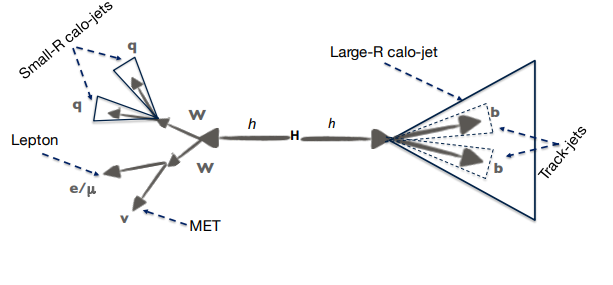
\includegraphics[scale=0.65]{figures/boosted_topo}
\caption{Diagram of the reconstructed event topology}
\label{fig:boost_topo}
\end{center}
\end{figure}

\subsection{Event Selection}
After the event is reconstructed, a b-jet veto is applied on the event by requiring all signal small-R jets do not pass b-tagging requirement to reject \ttbar events. The two highest \pT track-jets in the large-R jet are required to be b-tagged and events that passes this requirement is considered to be in the "2-tag" region. In addition, the \met is required to be more than 50 GeV to reject events from QCD multijet background. The cutflow for MC backgrounds and signal samples are documented in Appendix \ref{} and studies on the efficiency of the event reconstruction and selections can be found in Appendix \ref{}.

\subsection{Kinematic Selection}
\subsubsection{Signal Region}
\label{sec:boosted_regiondefs}
In order to enhance the sensitivity to a resonant HH signal, similarly to the resolved analysis, it is required
that the ${H\rightarrow b\overline{b}}$ candidate large-R jet has a mass consistent with the Standard Model Higgs boson mass.
Events which have the ${H\rightarrow b\overline{b}}$ candidate large-R jet mass in a window of ${90 \mathrm{GeV} < m_{\mathrm{Large-R jet}} < 140 \mathrm{GeV}}$ is considered to be in the signal region (SR).
The signal region is blinded and the blinding strategy is implemented by removing any events in data that passes the signal region requirement on the large-R jet mass.

\subsubsection{mBB Control Region}
In order to asses the modeling of the backgrounds, a control region is defined to be any events which fails the large-R jet signal region mass window requirement. Any event which has a large-R jet mass
 ${90 \mathrm{GeV} < m_{\mathrm{Large-R jet}}}$
 or ${m_{\mathrm{Large-R jet}} > 140 \mathrm{GeV}}$ 
 falls in the mBB control region (mBBcr). By construction, this region is orthogonal to the signal region.

\subsection{Multijet Background}
As with the resolved analysis, the QCD multijet background is estimated using the same data-driven method with slight modifications. 
 
The ABCD method uses three control regions (the B, C, and D regions) to estimate the contribution of a given background
in the signal (A) region.  Cuts on two ideally orthogonal variables are used to create the signal and various control regions,
e.g. the A region passes both cuts, the B and C regions each pass one cut and fail the other, while the D region fails both cuts.
 
For the boosted analysis, the ABCD regions are defined by using the same variables as in the resolved analysis, which are the significance of
the lepton impact parameter ($d_{0}^{\textrm{sig}}$) and the missing transverse momentum ($\met$). A small difference would be the higher cut value for the $\met$
with respect to the resolved analysis. The regions are defined as follow:
 
\begin{itemize}
\item Region A: \met > 50 GeV, $|d_{0}^{\textrm{sig}}|$ $<$ 2.0
\item Region B: \met < 50 GeV, $|d_{0}^{\textrm{sig}}|$ $<$ 2.0
\item Region C: \met > 50 GeV, $|d_{0}^{\textrm{sig}}|$ $>$ 2.0
\item Region D: \met < 50 GeV, $|d_{0}^{\textrm{sig}}|$ $>$ 2.0
\end{itemize}
 
\begin{figure}[!h]
\begin{center}
\includegraphics*[width=0.75\textwidth]{./figures/boosted/ABCD}
\caption{Regions defined in the ABCD method based on the lepton $d_{0}$ significance vs \met plane. Region A is the
signal enriched region which we want to estimate the multijet background. Region C is where the shape template is derived from and used
as shape prediction of the multijet background in region A. The ratio of the multijet yields in region B to region D is used to scale the multijet
yield in region C to predict the multijet background yield in region A.}
\label{fig:boosted_bkgd_abcd}
\end{center}
\end{figure}
 
Figure~\ref{fig:boosted_bkgd_abcd} shows the four regions represented on on the lepton $d_{0}$ significance vs \met plane.
Assuming that the two variables chosen to define the ABCD regions are completely uncorrelated, the QCD multijet yield in region A can be predicted. The The correlation between $|d_{0}^{\textrm{sig}}|$ vs \met is estimated in multiple MC background samples and also in data, and they are found to negligible (Appendix~\ref{app:boosted_qcd_d0met_plots}).
 
The ABCD method is done separately between the muon and electron channel as it is expected that the $\frac{N_B^\text{QCD}}{N_D^\text{QCD}}$ ratio and QCD multijet contribution to the total predicted background will be significantly different between the channels.
 
 %%%%%%%%%%%%%%%%%%%%%%%%%%%%%%%
%
% Yield prediction
%
%%%%%%%%%%%%%%%%%%%%%%%%%%%%%%%
\subsubsection{Yield prediction}
\label{sec:boosted_bkgd_qcdmultijet_yield}
 
Table~\ref{tab:boosted_region_bd_promptbkgd_data} lists the MC predicted prompt lepton backgrounds, observed data
and calculated multijet yields in Region B and D before the large-$R$ jet mass is applied and Table~\ref{tab:boosted_region_c_promptbkgd_data}
shows the yields in Region C mBB control region and signal region.
 
\begin{table}
\begin{center}
\begin{tabular}{l|c|c||c|c}
             &\multicolumn{2}{c||}{Region B}                &\multicolumn{2}{c}{Region D} \\
\hline
Samples       & Electron               & Muon                & Electron          & Muon \\      
\hline
$t\bar{t}$    &  307.7 $\pm$ 11.5      & 279.8 $\pm$ 10.6    & 21.3 $\pm$ 2.7    & 18.3  $\pm$ 2.6  \\
W+Jets        &  173.2 $\pm$ 5.2       & 179.3 $\pm$ 5.6     & 11.6 $\pm$ 1.4    & 10.6  $\pm$ 1.1  \\        
Single-top    &  42.9  $\pm$ 3.4       & 33.5  $\pm$ 3.6     &  3.0 $\pm$ 0.9    &  0.8  $\pm$ 0.5  \\
Z+Jets        &  78.5  $\pm$ 1.9       & 72.5  $\pm$ 1.7     &  6.4 $\pm$ 0.6    &  5.5  $\pm$ 0.5  \\
Dibosons      &  19.1  $\pm$ 1.5       & 17.7  $\pm$ 1.5     &  1.6 $\pm$ 0.4    &  2.2  $\pm$ 0.8  \\
\hline
Total Prompt  &  621.3 $\pm$ 13.2      & 582.7 $\pm$ 12.7    & 44.0 $\pm$ 3.3    & 37.4  $\pm$ 3.0  \\
\hline
Data          &  1003  $\pm$ 31.7      & 711   $\pm$ 26.7    & 144  $\pm$ 12.0   & 98    $\pm$ 9.9  \\
\hline
QCD           & 381.7 $\pm$ 34.3       & 128.3 $\pm$ 29.5    & 100.0 $\pm$ 12.4  & 60.6 $\pm$ 10.4 \\
\end{tabular}
\end{center}
\caption{MC predicted prompt lepton backgrounds, observed data and calculated multijet yields
in Region B and D. The multijet yield is calculated by subtracting the estimated total prompt lepton
backgrounds from the observed data. The statistical uncertainty on the yields is shown.}
\label{tab:boosted_region_bd_promptbkgd_data}
\end{table}
 
\begin{table}
\begin{center}
\begin{tabular}{l|c|c||c|c}
             &\multicolumn{2}{c||}{mBBcr}               &\multicolumn{2}{c}{SR}\\
\hline
Samples       & Electron            & Muon               & Electron         & Muon     \\      
\hline
$t\bar{t}$    &  38.7   $\pm$ 4.2   & 46.8  $\pm$ 7.9    & 28.5 $\pm$ 3.1   & 22.0 $\pm$ 2.7  \\
W+Jets        &  22.3   $\pm$ 2.0   & 20.0  $\pm$ 1.7    &  9.6 $\pm$ 1.3   & 10.0 $\pm$ 1.8  \\        
Single-top    &   7.6   $\pm$ 2.1   &  6.5  $\pm$ 1.3    &  7.1 $\pm$ 1.5   &  2.7 $\pm$ 0.8  \\
Z+Jets        &   4.6   $\pm$ 0.8   &  3.8  $\pm$ 0.5    &  1.6 $\pm$ 0.3   &  1.9 $\pm$ 0.6  \\
Dibosons      &   2.2   $\pm$ 0.6   &  1.2  $\pm$ 0.4    &  0.8 $\pm$ 0.3   &  1.7 $\pm$ 0.4  \\
\hline
Total Prompt  &  75.4   $\pm$ 5.2   & 78.4  $\pm$ 8.2    & 47.5 $\pm$ 3.7   & 38.3 $\pm$ 3.4  \\
\hline
Data          &  148    $\pm$ 12.2  & 126   $\pm$ 11.2   & 91   $\pm$ 9.5   & 71   $\pm$ 8.4  \\
\hline
QCD           & 72.6    $\pm$ 13.2  &  47.6 $\pm$ 13.9   & 43.5 $\pm$ 10.2  & 32.7 $\pm$ 9.1  \\
\end{tabular}
\end{center}
\caption{MC predicted prompt lepton backgrounds, observed data and calculated multijet yields
in Region C mBBcr and SR. The multijet yield is calculated by subtracting the estimated total prompt lepton
backgrounds from the observed data. The statistical uncertainty on the yields is shown.}
\label{tab:boosted_region_c_promptbkgd_data}
\end{table}
 
The $\frac{N_B^\text{QCD}}{N_D^\text{QCD}}$ ratio are calculated inclusively in the large-$R$ jet mass distribution.
In other words, the ratio is calculated without the jet mass window selection, which defines the SR and mBBcr, applied.
The ratio is then used to scale the QCD multijet yield in the SR and mBBcr of region C to predict the QCD multijet yield
in region A.
 
Table~\ref{tab:boosted_bkgd_abcd_ratio} shows the ratio in the electron channel and muon channel. As expected,
the electron channel ratio is larger than the muon channel. The muon channel ratio has a larger uncertainty due to
the more limited statistics in region B and region D compared to the electron channel. The predicted yields of the QCD multijet background
in the mBB control region and signal region are presented in Table~\ref{tab:boosted_bkgd_abcd_yield}. The QCD multijet background is
estimated to be ~19\% of the total background in the signal region (Table~\ref{tab:boosted_results_sr_yields}).
 
\begin{table}
\begin{center}
\begin{tabular}{c|c|c}
Multijet yield in region              & Electron                & Muon   \\      
\hline
$N_B^\text{QCD}$                      & 381.7 $\pm$ 34.3      & 128.3 $\pm$ 29.5 \\
$N_D^\text{QCD}$                      & 100.0 $\pm$ 12.4      & 60.6 $\pm$ 10.4  \\
\hline
$N_{B}^\text{QCD}$/$N_{D}^\text{QCD}$     & 3.8 $\pm$ 0.6 (15.3\%) & 2.1 $\pm$ 0.6 (28.7\%)   \\
\end{tabular}
\end{center}
\caption{Multijet yields in region B and region D and also the ratio of the yields for each lepton channel. The error
on the $\frac{N_B^\text{QCD}}{N_D^\text{QCD}}$ ratio is propagated from the statistical uncertainties on the multijet yields in each region.}
\label{tab:boosted_bkgd_abcd_ratio}
\end{table}
 
\begin{table}[!htbp]
\begin{center}
\begin{tabular}{c|c|c}
Multijet yield in region & Electron  & Muon  \\  
\hline
\multicolumn{3}{c}{SR} \\
\hline
$N_C^\text{QCD}$         & 43.4  $\pm$ 10.2 & 32.7 $\pm$ 9.1 \\
$N_A^\text{QCD}$         & 165.9 $\pm$ 46.6 (28.1\%) & 69.3 $\pm$ 27.7 (39.9\%) \\
\hline
\multicolumn{3}{c}{mBBcr} \\
\hline
$N_C^\text{QCD}$       & 72.6  $\pm$ 13.2 & 47.6  $\pm$ 13.9  \\
$N_A^\text{QCD}$       & 277.1 $\pm$ 66.0 (23.8\%) & 100.8 $\pm$ 41.3 (41.0\%)  \\
\hline
\end{tabular}
\end{center}
\caption{Multijet yield in region C and predicted yield in region A in the SR. The error on $N_A^\text{QCD}$
are propagated from the error on the $N_B^\text{QCD}$/$N_D^\text{QCD}$ ratio and statistical uncertainty on $N_C^\text{QCD}$ yield.
The numbers in brackets are the relative uncertainty in percentage.}
\label{tab:boosted_bkgd_abcd_yield}
\end{table}
 
\FloatBarrier
 
%%%%%%%%%%%%%%%%%%%%%%%%%%%%%%%
%
% Shape prediction
%
%%%%%%%%%%%%%%%%%%%%%%%%%%%%%%%
\subsubsection{Shape prediction}
\label{sec:boosted_bkgd_qcdmultijet_shape}
In order to predict the shape of the HH mass distribution (and also other kinematic distribution) of the QCD multijet background, the shape template of all kinematic distributions are obtained by subtracting all the MC backgrounds from data
in region C.
 
It was found that distributions in region C suffer from lack of statistics due the low number of data events which results in shape templates with severe statistical fluctuations. To overcome this, the shape templates are derived from a sample of 1 $b$-tagged (1-tag) events in region C. This sample requires that one of the two leading track-jet is $b$-tagged but not both at the same time. Comparisons between 2-tag and 1-tag shape templates are documented in Appendix~\ref{app:boosted_qcd_2tag1tag}.
 
%%%%%%%%%%%%%%%%%%%%%%%%%%%%%%%
%
% Normalization Uncertainties
%
%%%%%%%%%%%%%%%%%%%%%%%%%%%%%%%
\subsubsection{Multijet yield uncertainties}
\label{sec:boosted_bkgd_qcdmultijet_yield_unc}
 
%%%%%%%%%%%%%%%%%%%%%%%%%%%%%%%
% Statistical
%%%%%%%%%%%%%%%%%%%%%%%%%%%%%%%
\paragraph{Statistical} 
The uncertainty on the predicted yield of the multijet background is determined by propagating the statistical uncertainty
of the $\frac{N_B^\text{QCD}}{N_D^\text{QCD}}$ ratio, as shown in Table~\ref{tab:boosted_bkgd_abcd_ratio}, and the statisical
uncertainty on the multijet yield in region C ($N_C^\text{QCD}$), as in Table~\ref{tab:boosted_bkgd_abcd_yield}.
 
\paragraph{1-tag/2-tag jet mass acceptance} 
Another source of uncertainty on the multijet yield is the  
the difference of acceptance of the large-$R$ jet mass cut between 1-tag and 2-tag.
This uncertainty is included since the template for or the multijet shape prediction uses the multijet shape
from the 1-tag region C. Table~\ref{tab:boosted_syst_qcd_norm_mBBAcc} shows the acceptance
of the large-$R$ jet mass signal and mBB control region selection in the multijet 1-tag region C and 2-tag region C yields.
The relative difference between the acceptance in 1-tag region C and in 2-tag region C is considered as an uncertainty on the normalization
of the QCD multijet prediction.
 
\begin{table}[!htbp]
\begin{center}
\begin{tabular}{c|c|c}
\hline
Region    & Electron          & Muon      \\
\hline
\multicolumn{3}{c}{SR} \\
\hline
1-tag $\frac{N_\text{SR}}{N_\text{Inc}}$ &  31.6 $\pm$ 2.7 \% & 27.9 $\pm$ 2.7 \% \\
2-tag $\frac{N_\text{SR}}{N_\text{Inc}}$ &  37.5 $\pm$ 9.7 \% & 40.7 $\pm$ 9.7 \% \\
\hline \hline
Rel. difference between 1-tag and 2-tag & 15.6 \% & 31.5 \% \\
\hline
\multicolumn{3}{c}{mBBcr} \\
\hline
1-tag $\frac{N_\text{mBBcr}}{N_\text{Inc}}$ &  68.4 $\pm$ 2.7  \% & 72.1 $\pm$ 2.7 \% \\
2-tag $\frac{N_\text{mBBcr}}{N_\text{Inc}}$ &  62.5 $\pm$ 7.0  \% & 59.3 $\pm$ 7.0 \% \\
\hline \hline
Rel. difference between 1-tag and 2-tag &  9.4 \% &   21.6 \% \\
\end{tabular}
\end{center}
\caption{The acceptance of the large-$R$ jet mass signal region selection on the multijet
1-tag and 2-tag region C. $N_\text{SR}$($N_\text{Inc}$) is the multijet yield
with (without) the signal region large-$R$ jet mass selection.}
\label{tab:boosted_syst_qcd_norm_mBBAcc}
\end{table}
 
%%%%%%%%%%%%%%%%%%%%%%%%%%%%%%%
% mBB control region fit
%%%%%%%%%%%%%%%%%%%%%%%%%%%%%%%
\paragraph{mBB control region fit} 
 A likelihood fit of the large-$R$ jet mass in the mBB control region
is performed with the normalization of the multijet background to be unconstrained in the fit.
This study is documented in Appendix~\ref{app:boosted_qcd_float_2tag_mbbcr_fit}. In the muon channel,
the post-fit normalization factor is consistent with unity and in the electron channel,
the normalization factor is 0.676 $\pm$ 0.130. Due to this significant deviation from unity for the electron channel,
we assign a normalization uncertainty of 32.4\% for the multijet background in both the mBB control
region and signal region.
 
%%%%%%%%%%%%%%%%%%%%%%%%%%%%%%%
% ttbar and W+jets MC modeling
%%%%%%%%%%%%%%%%%%%%%%%%%%%%%%%
\paragraph{$t\bar{t}$ and W+jets MC modeling}
 The uncertainties on the MC modeling
of the $t\bar{t}$ and W+jets, the two largest prompt background predicted by MC in region B,D and C
are taken as a systematic on the predicted multijet background in region A since the multijet
background is calculated by subtracting the prompt background from observed data. The uncertainties
on the normalization of $t\bar{t}$ and W+jets in each region are calculated by comparing the yields
between the nominal $t\bar{t}$ and W+jets samples with their alternative samples
(see Section~\ref{sec:boosted_syst_modeling_top} and~\ref{sec:boosted_syst_modeling_vjets}).
The comparisons are documented in Appendix~\ref{app:boosted_qcd_region_mcmodeling_unc}.
 
The uncertainty on the multijet yield prediction in region A is then calculated
by recalculating the multijet yield in each region with the $t\bar{t}$ and W+jets
yields be varied up and down, simultaneously in all regions, by the uncertainty due to the
MC modeling of the background. The resulting multijet yield prediction in region A for
each background uncertainty is then compared to the nominal prediction in region A and the difference is
then taken as the uncertaintyon the multijet yield prediction in region A.
Table~\ref{tab:boosted_syst_qcd_norm_ttbarwjetsregionc} shows the uncertainty on the multijet yield prediction
in region A signal and mBB control region  due to the the uncertainty on the $t\bar{t}$ and W+jets
MC modeling.
 
\begin{table}[!htbp]
\begin{center}
\begin{tabular}{c|c|c}
& Electron  & Muon  \\  
\hline
\multicolumn{3}{c}{SR} \\
\hline
$t\bar{t}$           &     26.5 \% &   60.1 \%  \\
W+jets               &     24.7 \% &   70.4 \%  \\
\hline
\multicolumn{3}{c}{mBBcr} \\
\hline
$t\bar{t}$           &  37.4  \%  &   101.0\%  \\
W+jets               &  29.5  \%  &   77.6\%   \\
\hline
\end{tabular}
\end{center}
\caption{The uncertainty on the multijet yield prediction in region A due to the normalization
uncertainty of the $t\bar{t}$ and W+jets backgrounds in region C.}
\label{tab:boosted_syst_qcd_norm_ttbarwjetsregionc}
\end{table}
 
%%%%%%%%%%%%%%%%%%%%%%%%%%%%%%%
% Detector modeling
%%%%%%%%%%%%%%%%%%%%%%%%%%%%%%%
\paragraph{Detector modeling of prompt backgrounds}
 The detector modeling systematic uncertainties
on the prompt background in regions B, D and C are propagated through the ABCD method to estimate
the uncertainty on the multijet yield prediction region A. Table~\ref{tab:boosted_syst_qcd_norm_detmodel}
shows the uncertainties on the predicted multijet yield in both lepton channels. The impact of each detector
modeling systematics on the predicted multijet yield are listed in Appendix~\ref{app:boosted_qcd_prompt_detector_modeling_unc}.
 
\begin{table}[!htbp]
\begin{center}
\begin{tabular}{c|c|c}
& Electron  & Muon  \\  
\hline
\multicolumn{3}{c}{SR} \\
\hline
Total Uncertainty          &  46.0\%  &  105.6\%   \\
\hline
\multicolumn{3}{c}{mBBcr} \\
\hline
Total Uncertainty          &  45.5\%  &  127.3  \%   \\
\hline
\end{tabular}
\end{center}
\caption{The total uncertainty on the multijet yield prediction in region A due to the detector modeling
uncertainties of the prompt backgrounds in region B, C and D.}
\label{tab:boosted_syst_qcd_norm_detmodel}
\end{table}
 
%%%%%%%%%%%%%%%%%%%%%%%%%%%%%%%
% d0sig cut efficiency
%%%%%%%%%%%%%%%%%%%%%%%%%%%%%%%
\paragraph{$|d_{0}^{\textrm{sig}}|$ cut efficiency modeling}
The $|d_{0}^{\textrm{sig}}|$ cut efficiency modeling uncertainty for the prompt MC backgrounds
are also taken into account in the ABCD method due to the tigther cut on the leptons' $|d_{0}^{\textrm{sig}}|$,
than the recommended value. The determination of the $|d_{0}^{\textrm{sig}}|$ cut efficiency modeling uncertainty
is discussed in Section~\ref{sec:boosted_syst_d0cut}. This uncertainty is propagated through the ABCD method
by varying the normalization of the prompt backgrounds in regions B, D and C simultaneously to estimate
the uncertainty on the multijet yield prediction region A and is treated as anti-correlated between regions B and regions D,C.
Table~\ref{tab:boosted_syst_qcd_norm_d0sigacc} shows the uncertainties on the predicted multijet yield due
$|d_{0}^{\textrm{sig}}|$ cut efficiency modeling uncertainty on prompt MC backgrounds in both lepton channels.
The breakdown of the multijet yield and its variation due to the $|d_{0}^{\textrm{sig}}|$ cut efficiency modeling uncertainty
on the prompt MC backgrounds in each region and channel is listed in Table~\ref{tab:boosted_qcd_d0syst_breakdown} of
Appendix~\ref{app:boosted_qcd_prompt_d0cut_modeling_unc}.
 
\begin{table}[!htbp]
\begin{center}
\begin{tabular}{c|c|c}
& Electron  & Muon  \\  
\hline
\multicolumn{3}{c}{SR} \\
\hline
Total Uncertainty          &  46.4\%  &  50.9\%   \\
\hline
\multicolumn{3}{c}{mBBcr} \\
\hline
Total Uncertainty          &  42.0\%  &  110.6\%   \\
\hline
\end{tabular}
\end{center}
\caption{The total uncertainty on the multijet yield prediction in region A due to the $|d_{0}^{\textrm{sig}}|$
cut efficiency modeling uncertainties of the prompt backgrounds in region B, D and C.}
\label{tab:boosted_syst_qcd_norm_d0sigacc}
\end{table}
 
%%%%%%%%%%%%%%%%%%%%%%%%%%%%%%%
% Total uncertainty
%%%%%%%%%%%%%%%%%%%%%%%%%%%%%%%
\paragraph{Total uncertainty on the yield}
 The total uncertainty on the multijet prediction
is calculated as the sum in quadrature of the uncertainties from the two sources explained above.
Table~\ref{tab:boosted_syst_qcd_norm_unc_final} summarizes the systematic uncertainties on the predicted
multijet yield in the electron channel and the muon channel.
 
\begin{table}[!htbp]
\begin{center}
\begin{tabular}{c|c|c}
Source of uncertainty &  Electron  & Muon  \\  
\hline
\multicolumn{3}{c}{SR} \\
\hline
Statistical                                      &  28.1 \% & 39.9 \% \\
2-tag/1-tag jet mass acceptance                  &  15.6 \% & 31.5 \% \\
mBB control region fit                           &  32.3 \% & - \\
$t\bar{t}$ MC modeling                          &  26.5 \% & 60.1\% \\
W+jets modeling                                 &  24.7 \% & 70.4\% \\
Detector modeling of prompt backgrounds         &  46.0 \% & 105.6\% \\
$|d_{0}^{\textrm{sig}}|$ cut efficiency          &  46.4 \% & 50.9\% \\
\hline
Total                                            &  87.5 \% & 157.8 \% \\
\hline
\hline
\multicolumn{3}{c}{mBBcr} \\
\hline
Statistical                                      &  23.8 \% & 41.0 \% \\
2-tag/1-tag jet mass acceptance                  &  9.4  \% & 21.6 \% \\
mBB control region fit                           &  32.3 \% & -       \\
$t\bar{t}$ MC modeling                          &  37.4 \% & 101.0\% \\
W+jets MC modeling                              &  29.5 \% & 77.6\% \\
Detector modeling of prompt backgrounds         &  45.5 \% & 127.3\% \\
$|d_{0}^{\textrm{sig}}|$ cut efficiency          &  42.0 \% & 110.6\% \\
\hline
Total                                            &  88.3 \% & 216.4 \% \\
\end{tabular}
\end{center}
\caption{Summary of systematic uncertainties on the QCD multijet yield in the signal region and mBB control region
for each lepton channel. The total uncertainty calculated by adding in quadrature the uncertainties from all sources.}
\label{tab:boosted_syst_qcd_norm_unc_final}
\end{table}
 
%%%%%%%%%%%%%%%%%%%%%%%%%%%%%%%
%
% Shape Uncertainties
%
%%%%%%%%%%%%%%%%%%%%%%%%%%%%%%%
\subsubsection{Multijet shape uncertainties}
\label{sec:boosted_bkgd_qcdmultijet_shape_unc}
 
The uncertainty on the $m_{HH}$ distribution prediction for the QCD multijet background is estimated by comparing
the $m_{HH}$ distribution shape in the 2-tag region C and 1-tag region C (Figure~\ref{fig:abcd_shapesyst}).
 
\begin{figure}[!h]
\begin{center}
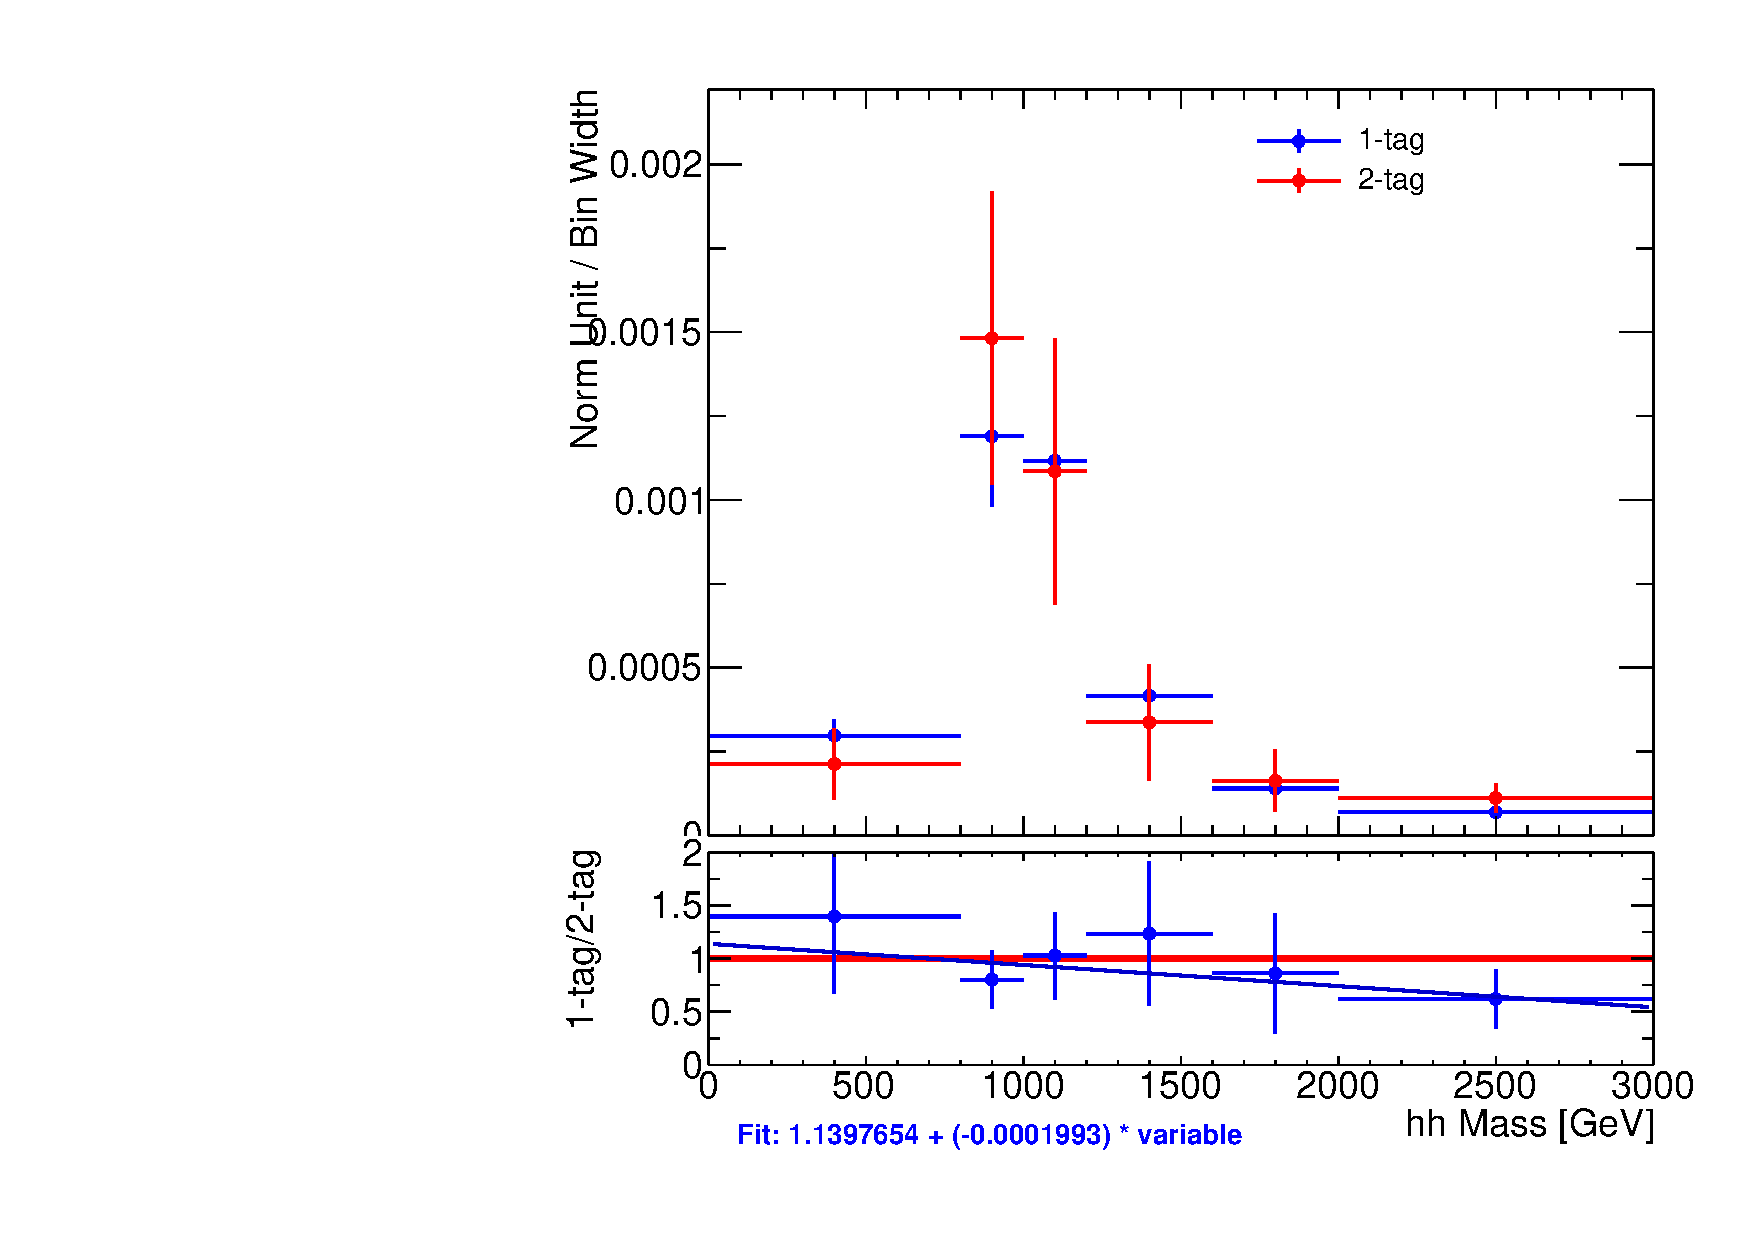
\includegraphics[scale=0.33]{./figures/boosted/ABCD/QCD_SR_hhMass.pdf}
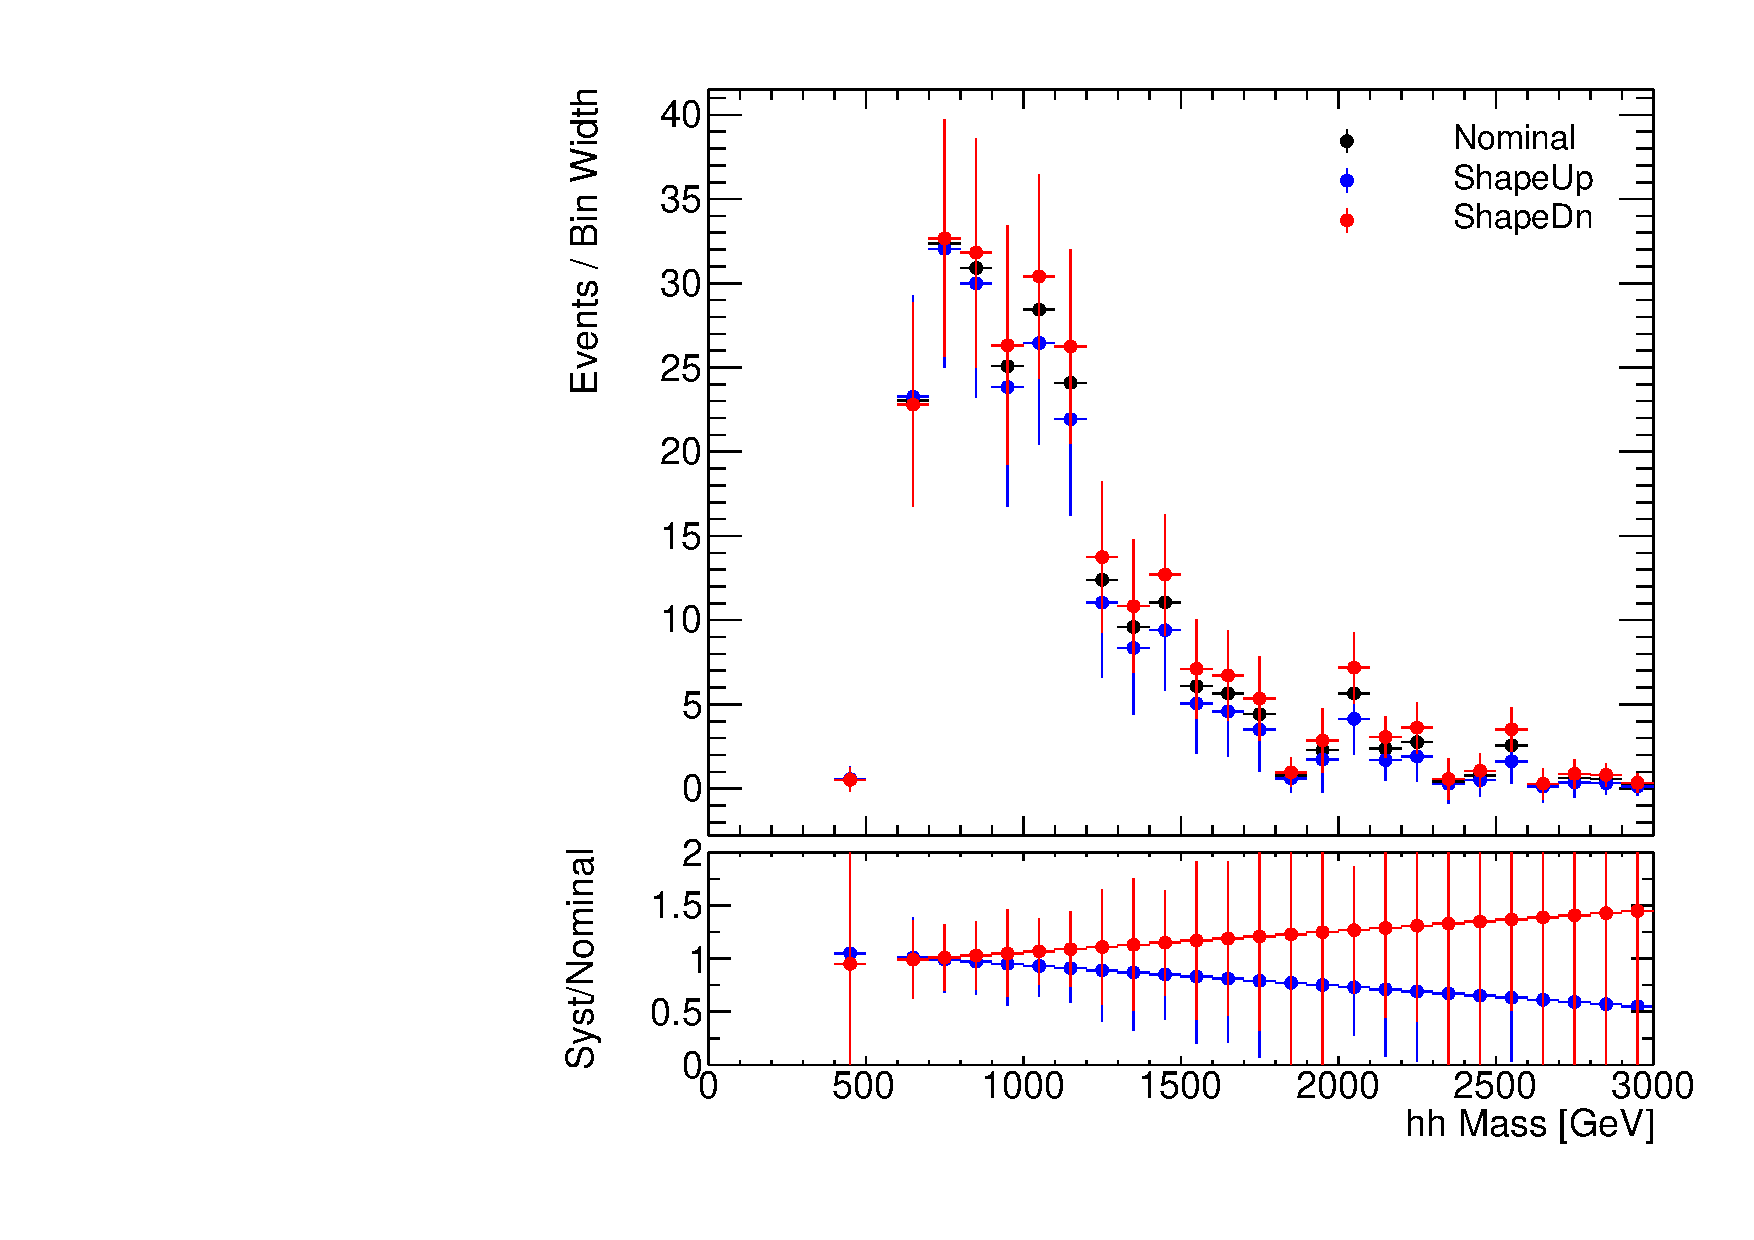
\includegraphics[scale=0.33]{./figures/boosted/ABCD/Fit_QCD_SR_hhMass.pdf}
\caption{(a) Shape comparison of the $m_{HH}$ distribution in region C of the 1-tag and 2-tag region.
The linear fit to the ratio is used as the shape systematic of QCD background prediction.
(b) The up and down QCD shape systematic variation for the predicted $m_{HH}$ distribution.}
\label{fig:boosted_abcd_shapesyst}
\end{center}
\end{figure}

%%%%%%%%%%%%%%%%%%%%%%%%%%%%%%%
%
% Final prediction
%
%%%%%%%%%%%%%%%%%%%%%%%%%%%%%%%
\subsubsection{Final prediction and validation}
\label{sec:boosted_bkgd_qcdmultijet_predict_valid}
 
The predicted multijet yield and its uncertainty in the signal region and mBB control region are
shown in Table~\ref{tab:boosted_syst_qcd_norm_unc}.
 
\begin{table}[!htbp]
\begin{center}
\begin{tabular}{l|c|c|c}
Region    & Electron                   & Muon                       & Combined                   \\  
\hline
SR        & 165.9 $\pm$ 145.2(87.5\%) & 69.3 $\pm$ 109.3(157.8\%)   & 235.2 $\pm$ 181.8 (77.3\%) \\
mBBcr     & 277.1 $\pm$ 244.8(88.3\%) & 100.8 $\pm$ 218.1(216.4\%)  & 377.9 $\pm$ 327.8 (86.8\%) \\
\hline
\end{tabular}
\end{center}
\caption{Predicted multijet yield with uncertainties in the signal region (SR) and mBB control region (mBBcr)
for each lepton channel.}
\label{tab:boosted_syst_qcd_norm_unc}
\end{table}
 
The ABCD method is validated by assesing the agreement of data and total background prediction with the QCD multijet background included
in the mBB control region. This is dicussed in Section~\ref{sec:boosted_bkgd_datavspred}.
 
%
% ttbar
%
\subsection{$t\bar{t}$}
\label{sec:boosted_bkgd_ttbar}
 
MC simulation is used to model the shape of the $t\bar{t}$ background. The background
is predicted to be the largest (\textasciitilde 52\%) of the total background. A top-enriched control region
is used to validate the modeling of the $t\bar{t}$ background and the comparison between Data and
background prediction is documented in Appendix~\ref{app:boosted_ttbarmodel_topcr}.
% The normalization of the $t\bar{t}$ background is obtained by fitting the large-$R$ jet mass distribution
% in the mBB control region and extract the normalization factor on the $t\bar{t}$ normalization from the fit.
% Both the $t\bar{t}$ and W+jets backgrounds are allowed to float simultaneously in the fit. The studies are documented in
% Appendix ~\ref{app:boosted_fitstudies_mBBcr}.
 
%
% V+jets
%
\subsection{V+jets}
\label{sec:boosted_bkgd_vjets}
 
MC simulation is used to model the shape and predict the yield of the W+jets and Z+jets background.
The W+jets background is predicted to be the third largest background (\textasciitilde 18\%) of the total background while
the Z+jets background is expected to be \textasciitilde 2\% in the signal region (Table~\ref{tab:boosted_results_sr_yields}).
 
%
% Single-top
%
\subsection{Single Top}
\label{sec:boosted_bkgd_singletop}
 
MC simulation is used to model the shape and predict the yield of background from single-top processes. This background is
predicted to be \textasciitilde 9\% of the total background (Table~\ref{tab:boosted_results_sr_yields}).
The single-top background is predominantly consist of Wt production process
(\textasciitilde 90\%), followed by the t-channel production (\textasciitilde 9\%) and the s-channel production (\textasciitilde 1\%).
 
%
% Diboson
%
\subsection{Diboson}
\label{sec:boosted_bkgd_diboson}
MC simulation is used to model the shape and predict the yield of the diboson background. This background is predicted to be
~2\% of the total background in the signal region  (Table~\ref{tab:boosted_results_sr_yields}).
 
 
\subsection{Data/Prediction comparisons in control regions}
\label{sec:boosted_bkgd_datavspred}
 
To asses the modeling of the background, the total predicted background is asses with data in the mBB control region.
The electron channel and the muon channel are combined into a single channel.
 
Table~\ref{tab:boosted_bkgd_mbbcr_yields} shows the predicted yield of each background. The data, collected in 2015+2016,
corresponding to the integrated luminosity of 36.1 fb$^{-1}$ are used. The MC backgrounds $t\bar{t}$, W+jets,
Single-top, Z+jets and Dibosons are normalized to luminosity. The QCD multijet prediction is estimated from the ABCD method.
Statistical errors are shown for the individual backgrounds and the total predicted background while the error due
to systematic uncertainties are shown only for the total predicted background. Detector modeling uncertainties, MC background modeling
uncertainties and uncertainties from the ABCD method for QCD multijet background are considered.
The predicted total background yield has an error of about 27\% due to systematic uncertainties and
the observed yield in data is in good agreement with the total background yield.
 
Figure~\ref{fig:boosted_mbbcr_mainplots}, \ref{fig:boosted_mbbcr_largerjet}, \ref{fig:boosted_mbbcr_wwsystem},
\ref{fig:boosted_mbbcr_whad}, \ref{fig:boosted_mbbcr_wlep}, \ref{fig:boosted_mbbcr_lepton}, \ref{fig:boosted_mbbcr_whad_jets}
and \ref{fig:boosted_mbbcr_dr} show the distributions of kinematic variables for events which fall into the mBB control regions.
The observed data (black circle) corresponds to an integrated luminosity of 36.1 fb$^{-1}$. The MC backgrounds $t\bar{t}$ (orange), W+jets (blue),
Single-top (red), Z+jets (green) and Dibosons (yellow) are normalized to cross-section prediction scaled to luminosity of 36.1 fb$^{-1}$.
The QCD multijet background (grey) is predicted from the ABCD method. The hashed grey band is the statistical uncertainty on
the predicted background and the red box band is the statistical+systematics uncertainty on the predicted background.
The systematics uncertainty on the predicted background consists of the detector modeling systematic uncertainties,
MC background modeling uncertainties and uncertainties from the ABCD method for QCD multijet background.
 
Figure~\ref{fig:boosted_mbbcr_mainplots} is the invariant mass of the reconstructed di-Higgs (hh)system distribution, the $\met$, and $W \to l\nu$ system transverse mass distributions and as it can be seen that it is reasonably modelled. The good modeling observed of the
distributions gives confidence to the QCD multijet prediction as the events from the background tend to have
low values of $\met$ and transverse mass.
 
In Appendix~\ref{app:boosted_mbbcontrolregion}, the kinematic distributions are shown separately in the low mBB and high mBB region
of the mBB control region (App.~\ref{app:boosted_mbbcontrolregion_highlow}). The distributions separated by the lepton channels are
also shown (App.~\ref{app:boosted_mbbcontrolregion_leptonchannels}).
 
\renewcommand{\arraystretch}{1.5}
\begin{table}
\begin{center}
\begin{tabular}{l|c|c|c}
Sample        &  Yield   &  Stats Unc &   Systs Unc \\
\hline
$t\bar{t}$    &  1005.6  & $\pm$ 20.6    &   $^{+283.6(+28.2\%)}_{-288.8(-28.7\%)}$ \\
W+Jets        &  565.6   & $\pm$ 10.3    &   $^{+277.9(+49.1\%)}_{-270.0(-47.7\%)}$ \\
QCD           &  377.9   & $\pm$ 19.6    &   $^{+328.0(+86.8\%)}_{-328.0(-86.8\%)}$ \\
Single-top    &  161.3   & $\pm$ 7.2     &   $^{+114.4(+70.9\%)}_{-114.4(-70.9\%)}$ \\
Z+Jets        &  55.9    & $\pm$ 1.6     &   $^{+27.7(+49.5\%)}_{-27.2(-48.6\%)}$ \\
Dibosons      &  39.7    & $\pm$ 2.6     &   $^{+23.4(+58.9\%)}_{-23.3(-58.7\%)}$ \\
\hline
Prediction    &  2206.0  & $\pm$ 31.2    &   $^{+593.7(+26.9\%)}_{-586.1(-26.6\%)}$ \\
Data          &  2179    & - & - \\
\hline
Data/Pred     &  0.99    & - & - \\
\hline
\end{tabular}
\end{center}
\caption{Predicted and observed yields in the mBB control region. Detector modeling
uncertainties, MC background modeling uncertainties and QCD background modeling uncertainties
from ABCD method are considered for the systematic uncertainties.}
\label{tab:boosted_bkgd_mbbcr_yields}
\end{table}
\renewcommand{\arraystretch}{1.0}
 
\begin{figure}[!h]
\begin{center}
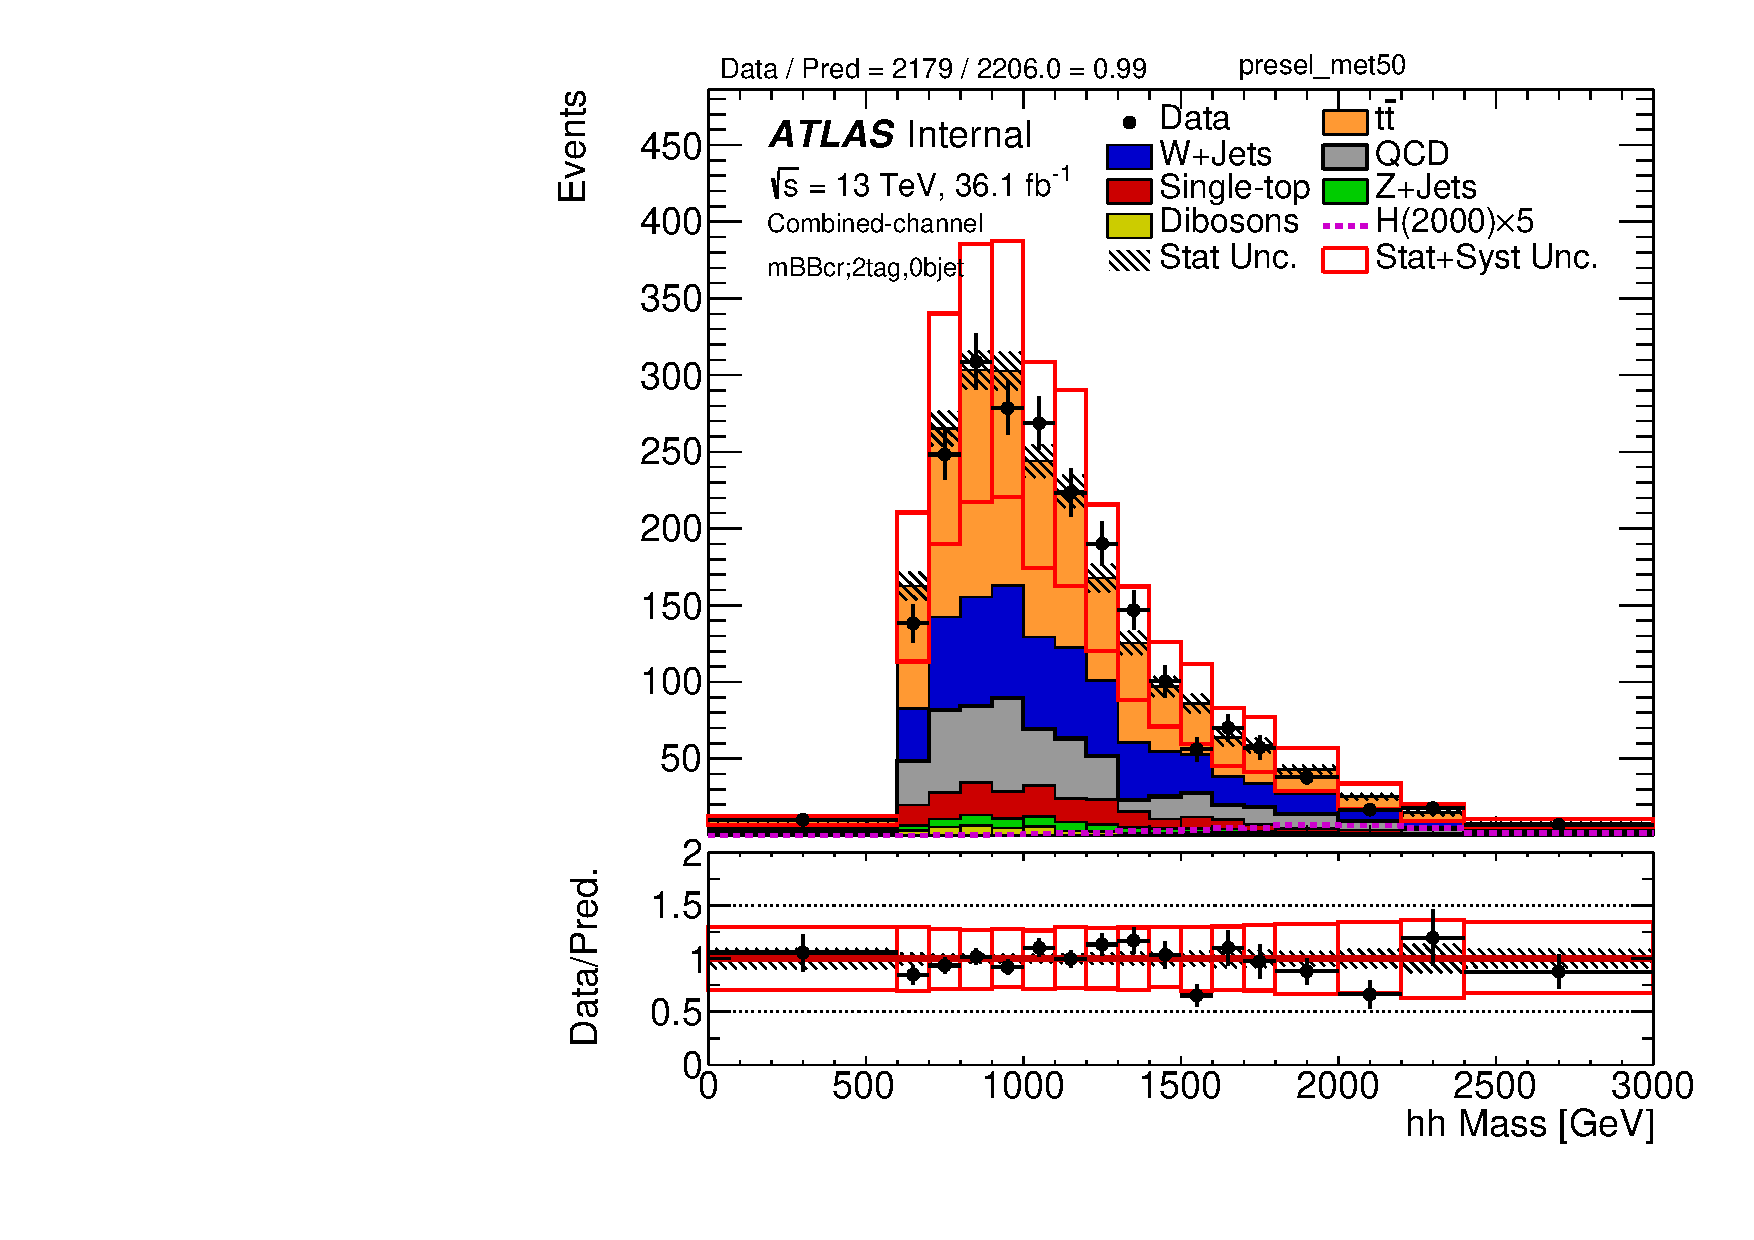
\includegraphics[scale=0.33]{./figures/boosted/PlotsInMbbCR/DataMC_2tag_0bjet_mbbcr_lepton_presel_met50_hhMassRebin1}
\par\medskip
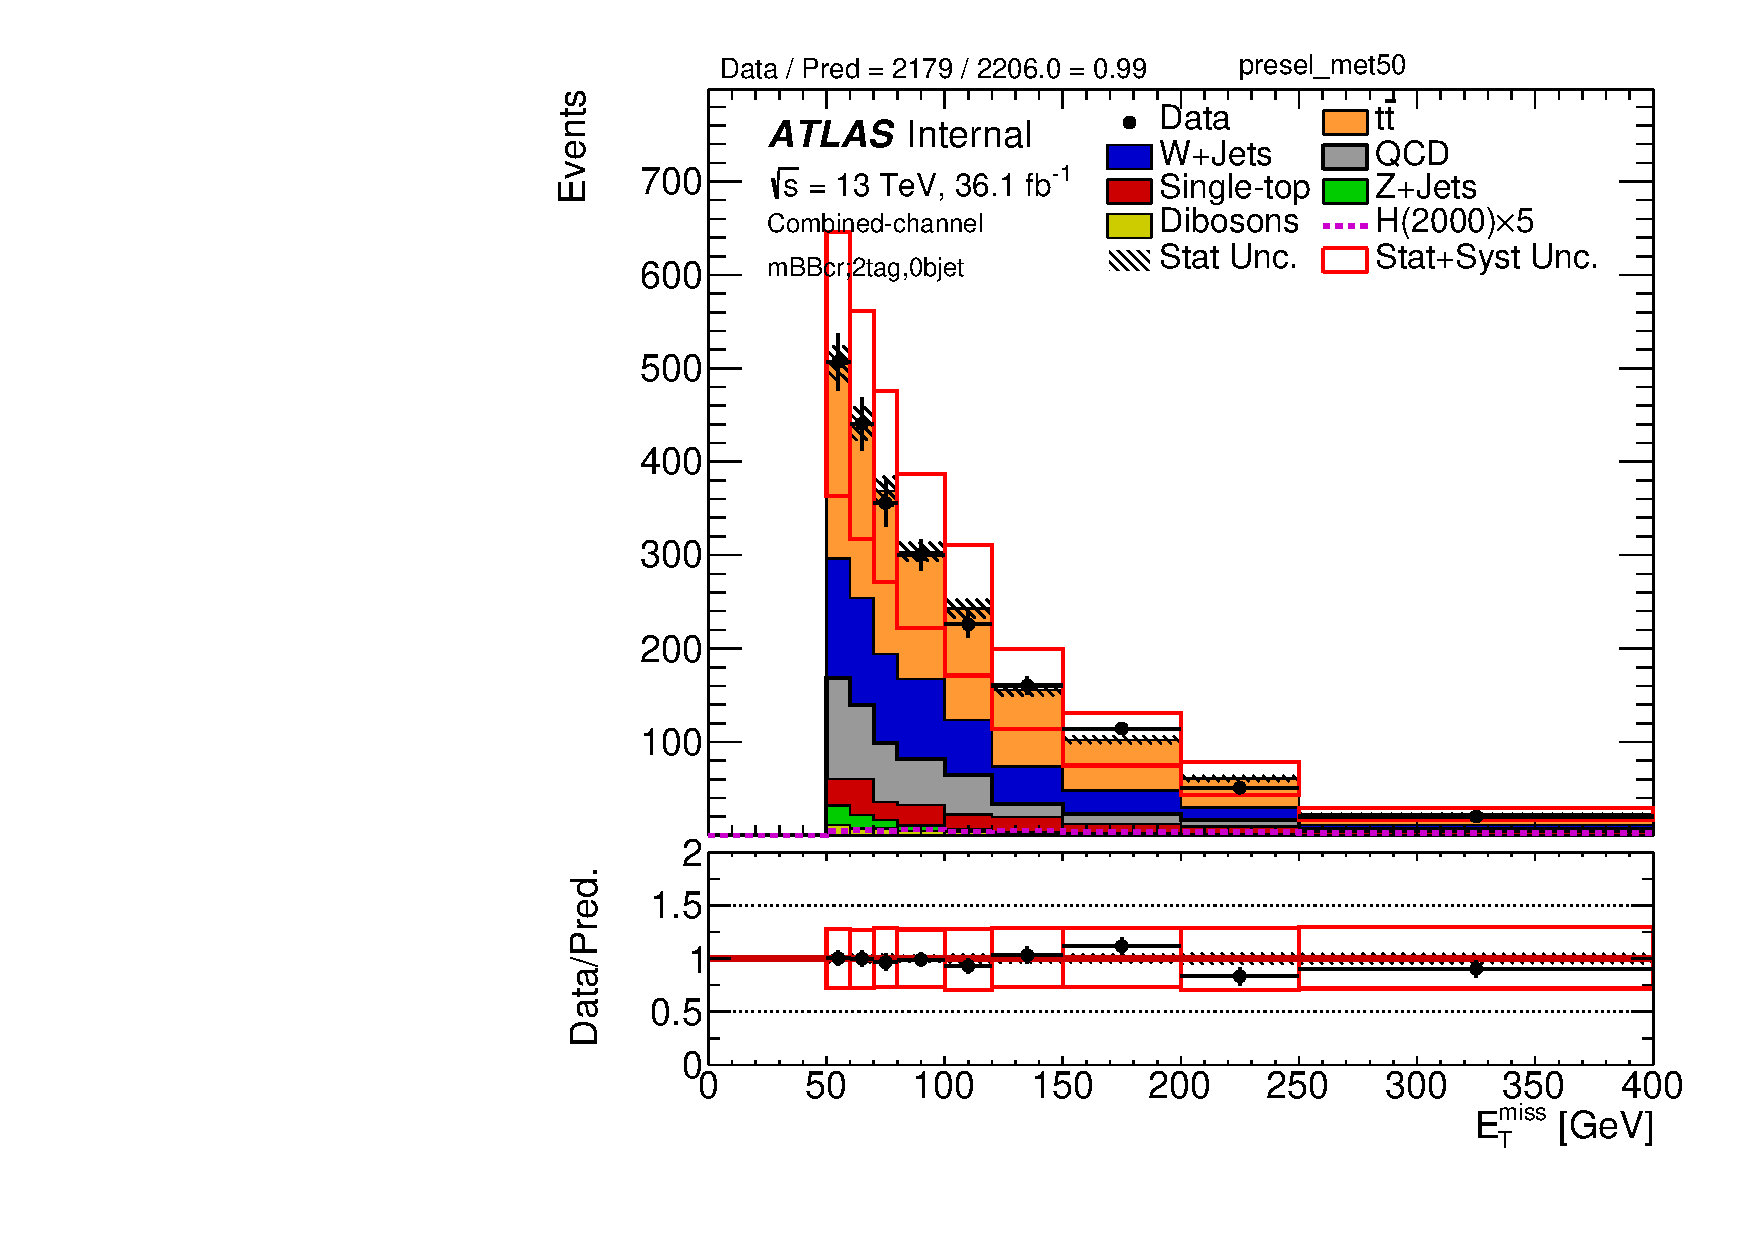
\includegraphics[scale=0.33]{./figures/boosted/PlotsInMbbCR/DataMC_2tag_0bjet_mbbcr_lepton_presel_met50_MET}
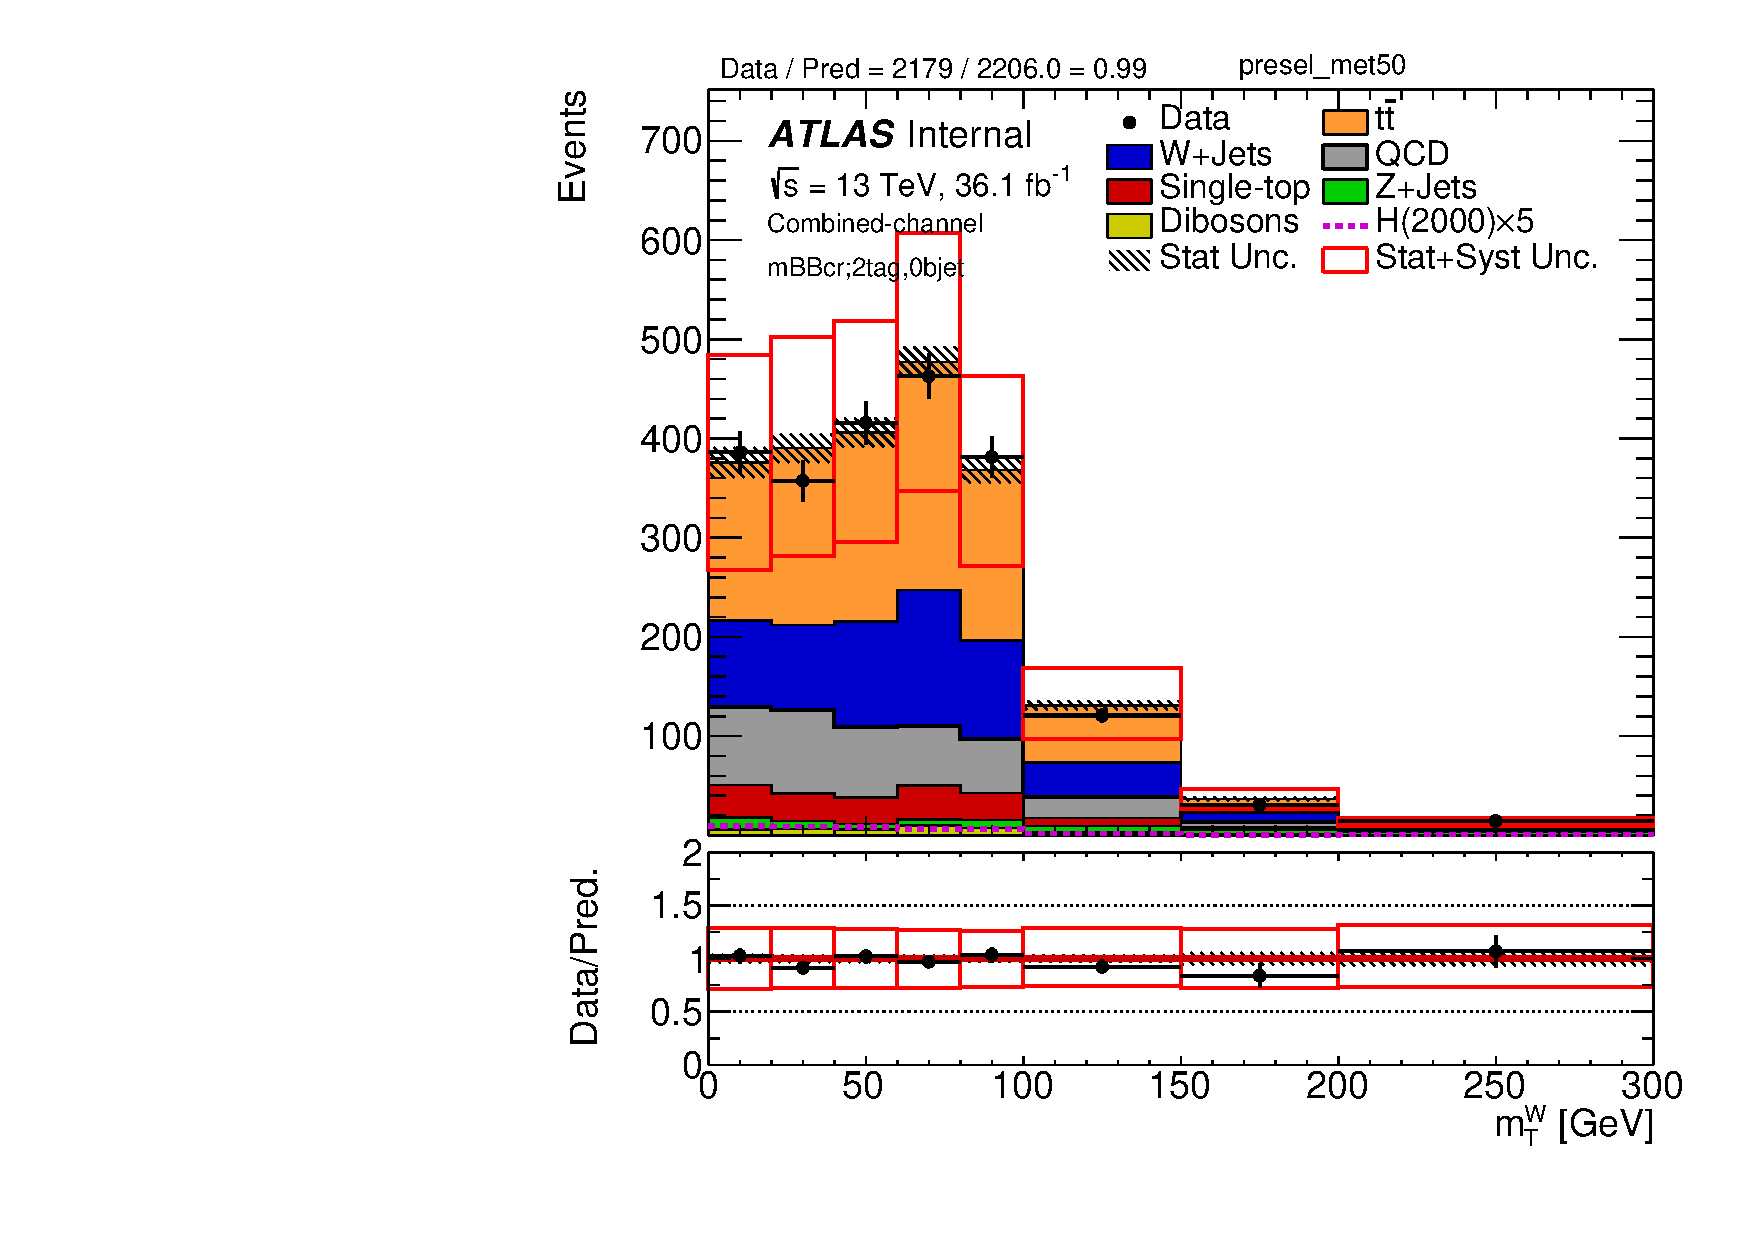
\includegraphics[scale=0.33]{./figures/boosted/PlotsInMbbCR/DataMC_2tag_0bjet_mbbcr_lepton_presel_met50_WlepMtATLAS}
\caption{The invariant mass of the reconstructed di-Higgs (hh) system, \met and transverse mass of the $W \to l\nu$ system
distributions of events in the mBB control region (mBBcr).}
\label{fig:boosted_mbbcr_mainplots}
\end{center}
\end{figure}
% 
\begin{figure}[!h]
\begin{center}
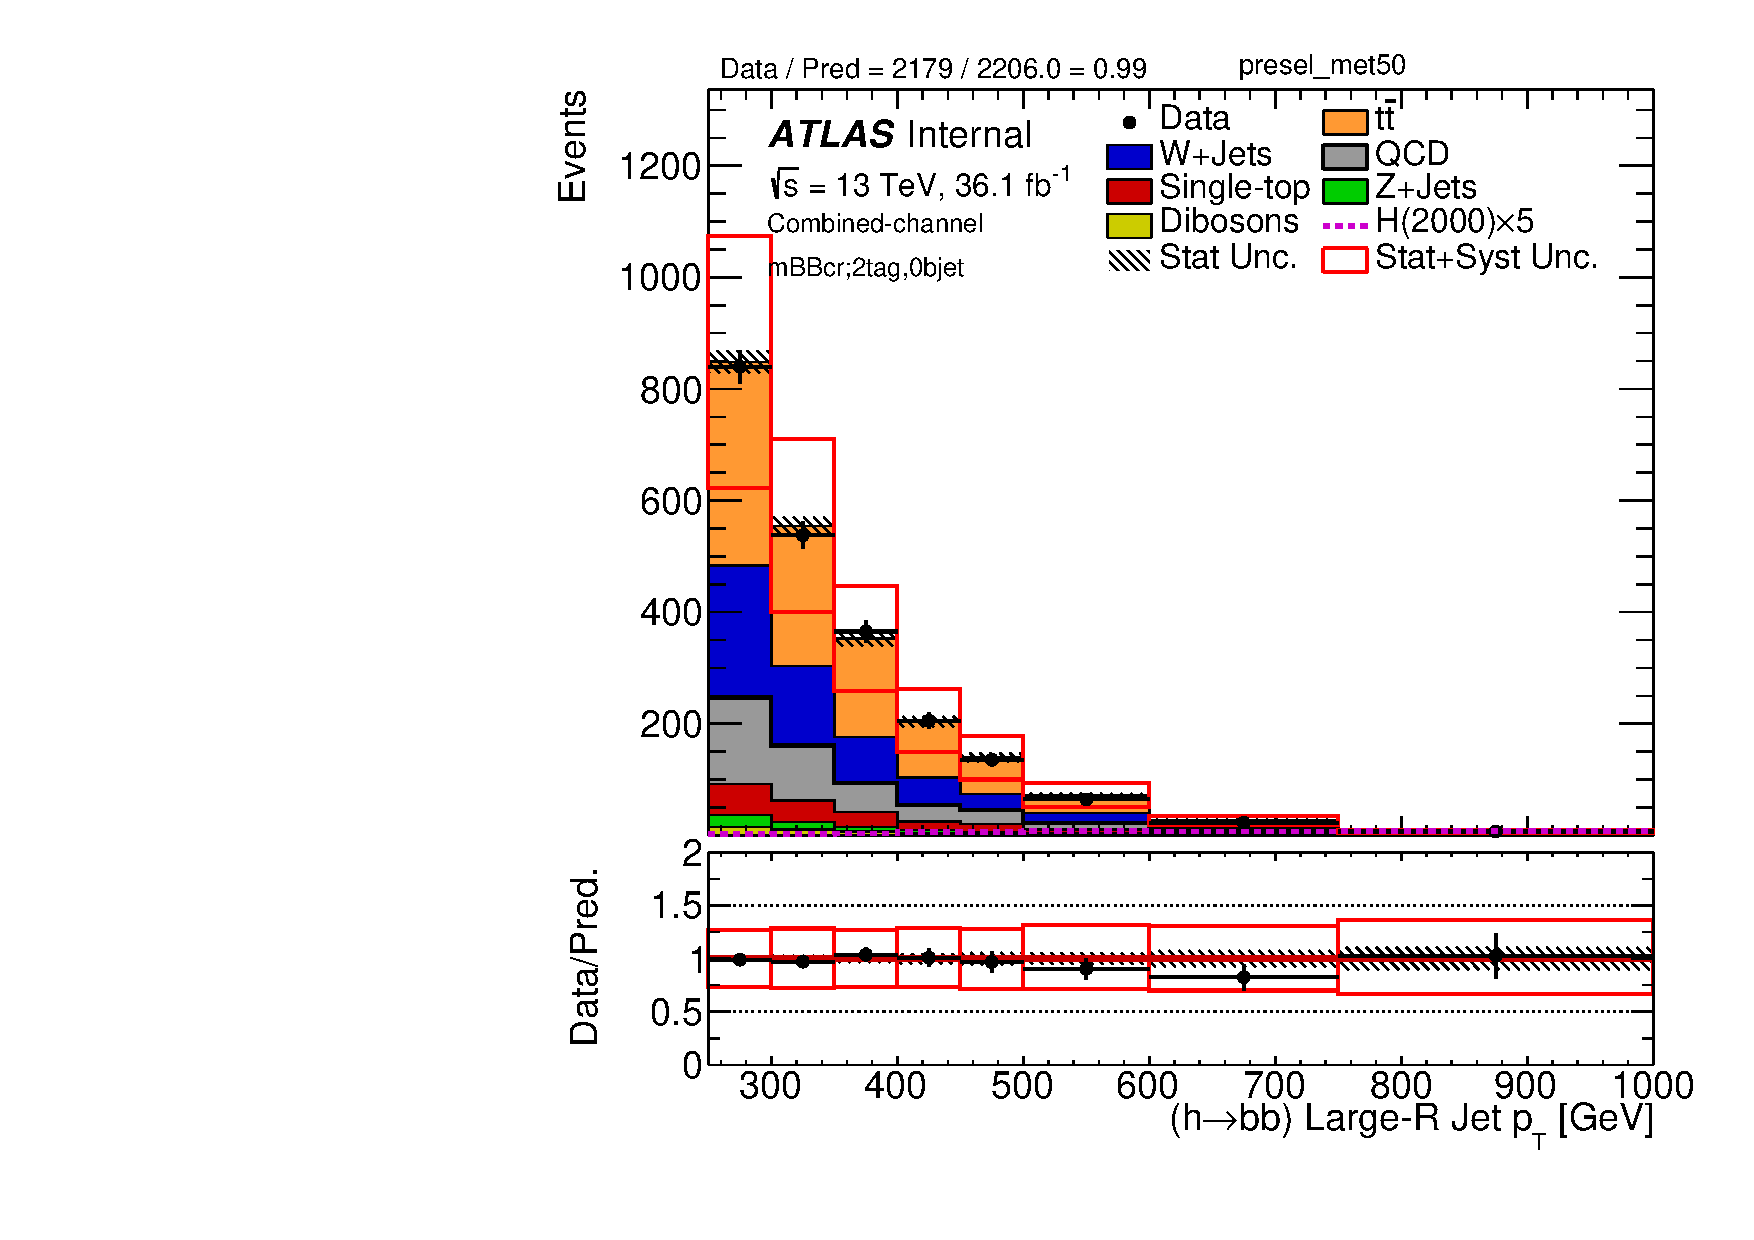
\includegraphics[scale=0.33]{./figures/boosted/PlotsInMbbCR/DataMC_2tag_0bjet_mbbcr_lepton_presel_met50_HbbPt}
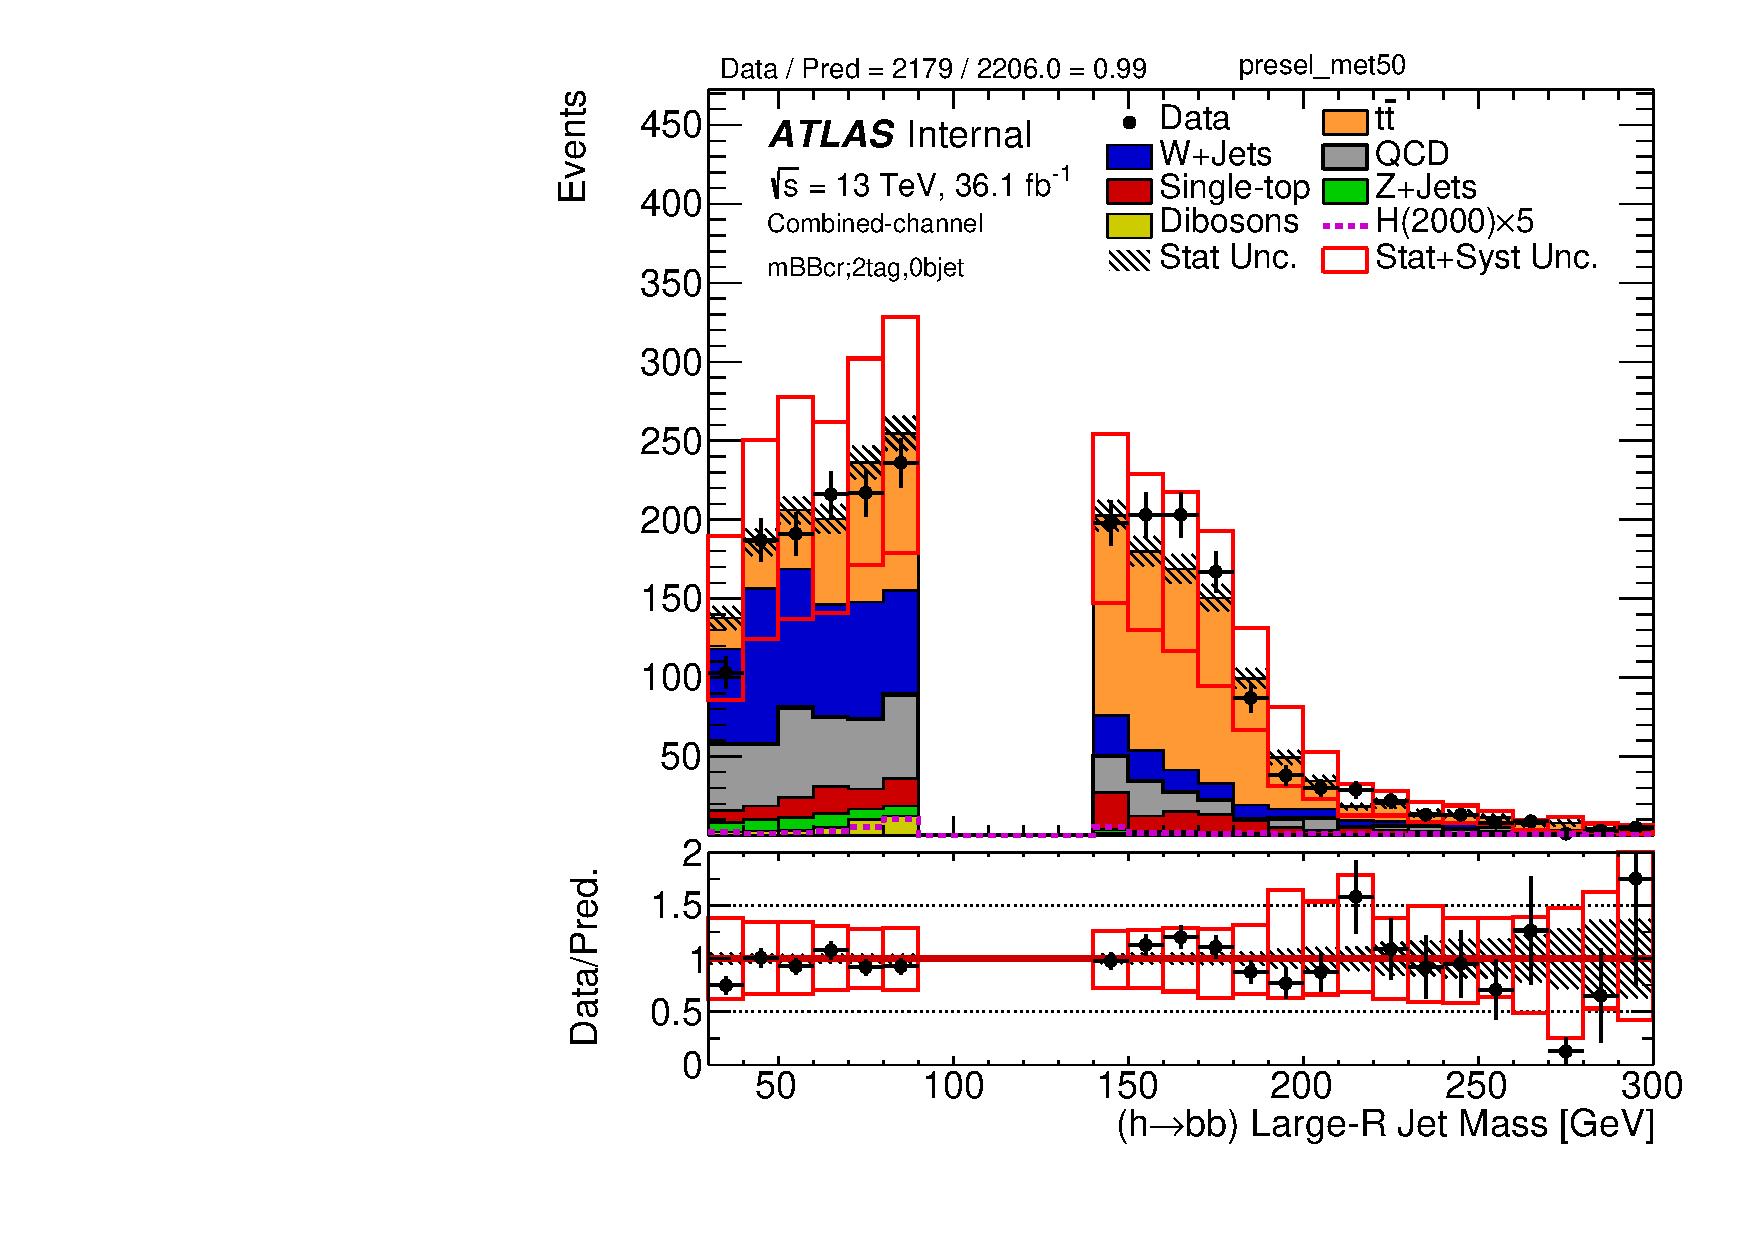
\includegraphics[scale=0.33]{./figures/boosted/PlotsInMbbCR/DataMC_2tag_0bjet_mbbcr_lepton_presel_met50_HbbMass} \\
\par\medskip
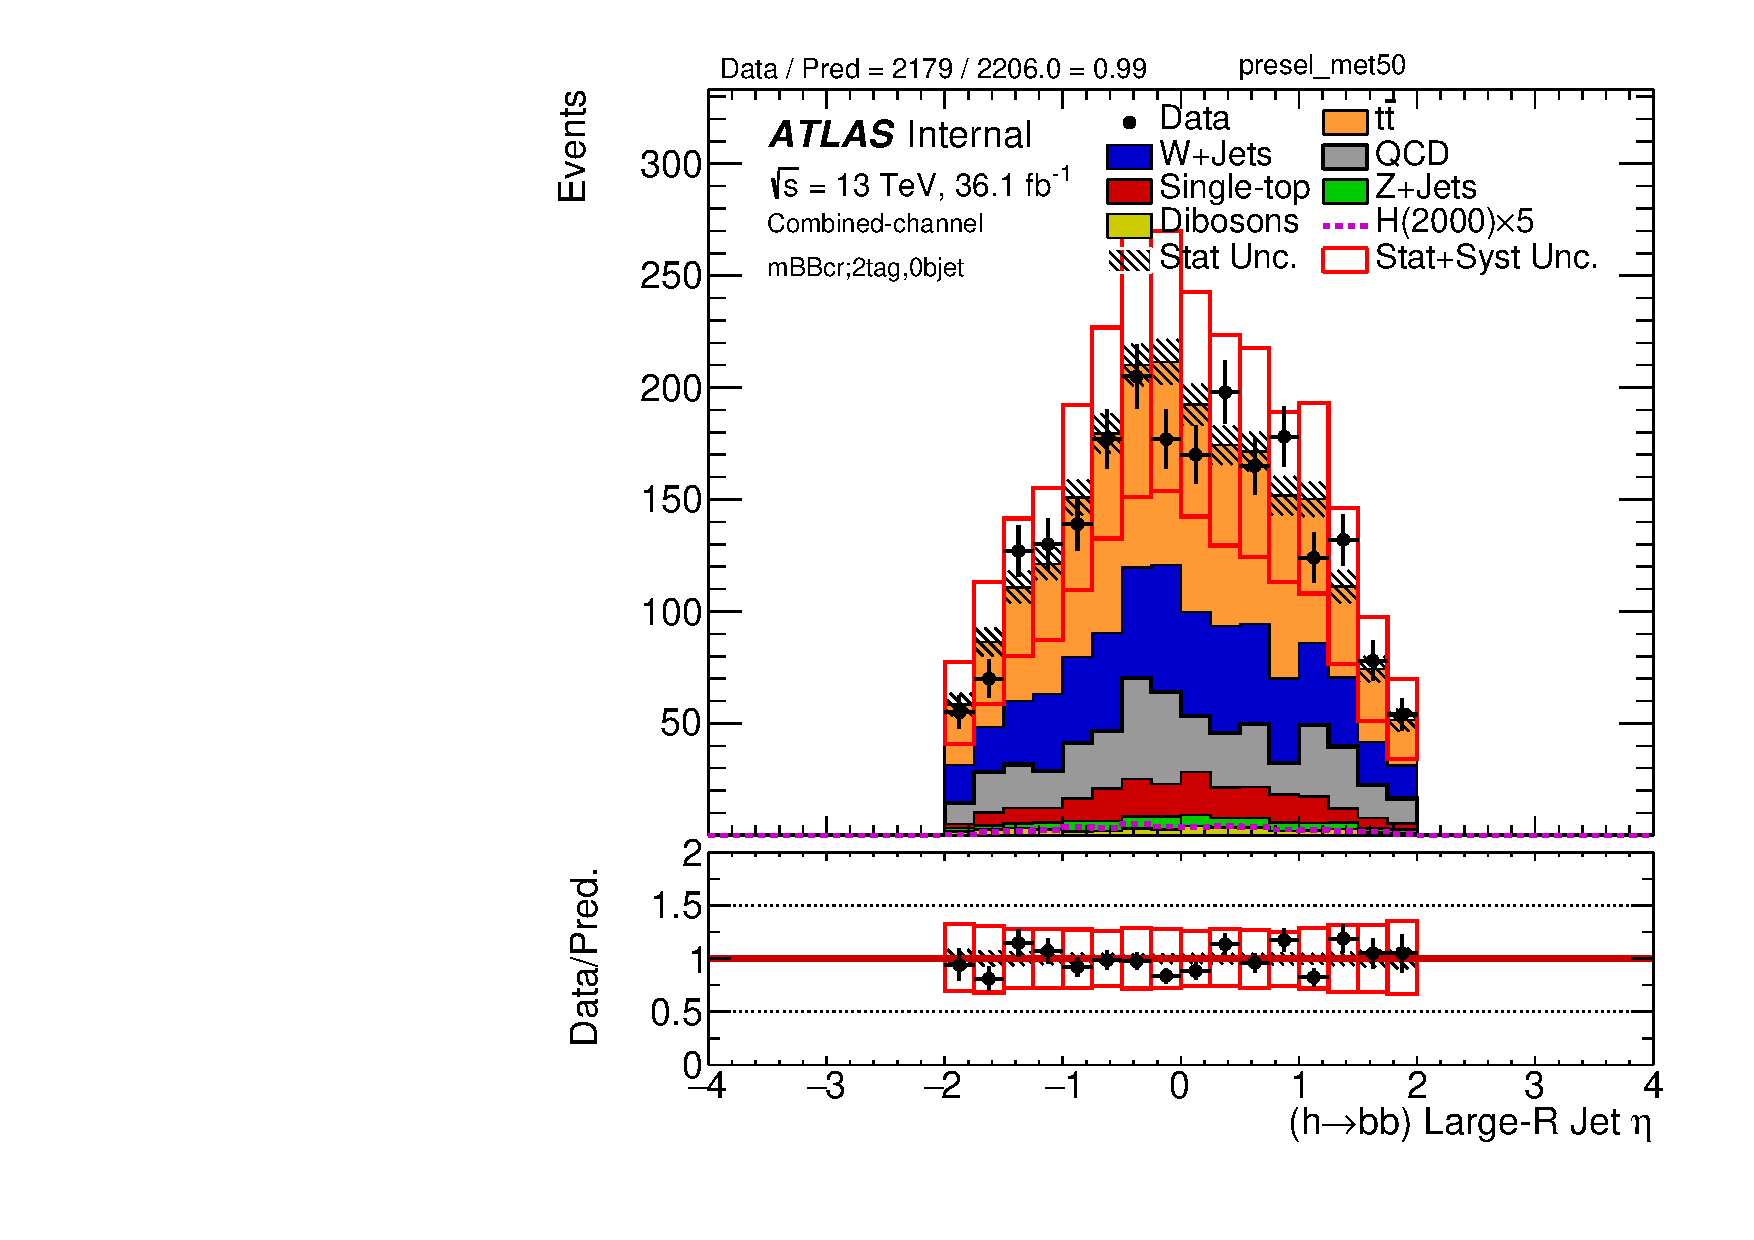
\includegraphics[scale=0.33]{./figures/boosted/PlotsInMbbCR/DataMC_2tag_0bjet_mbbcr_lepton_presel_met50_HbbEta} 
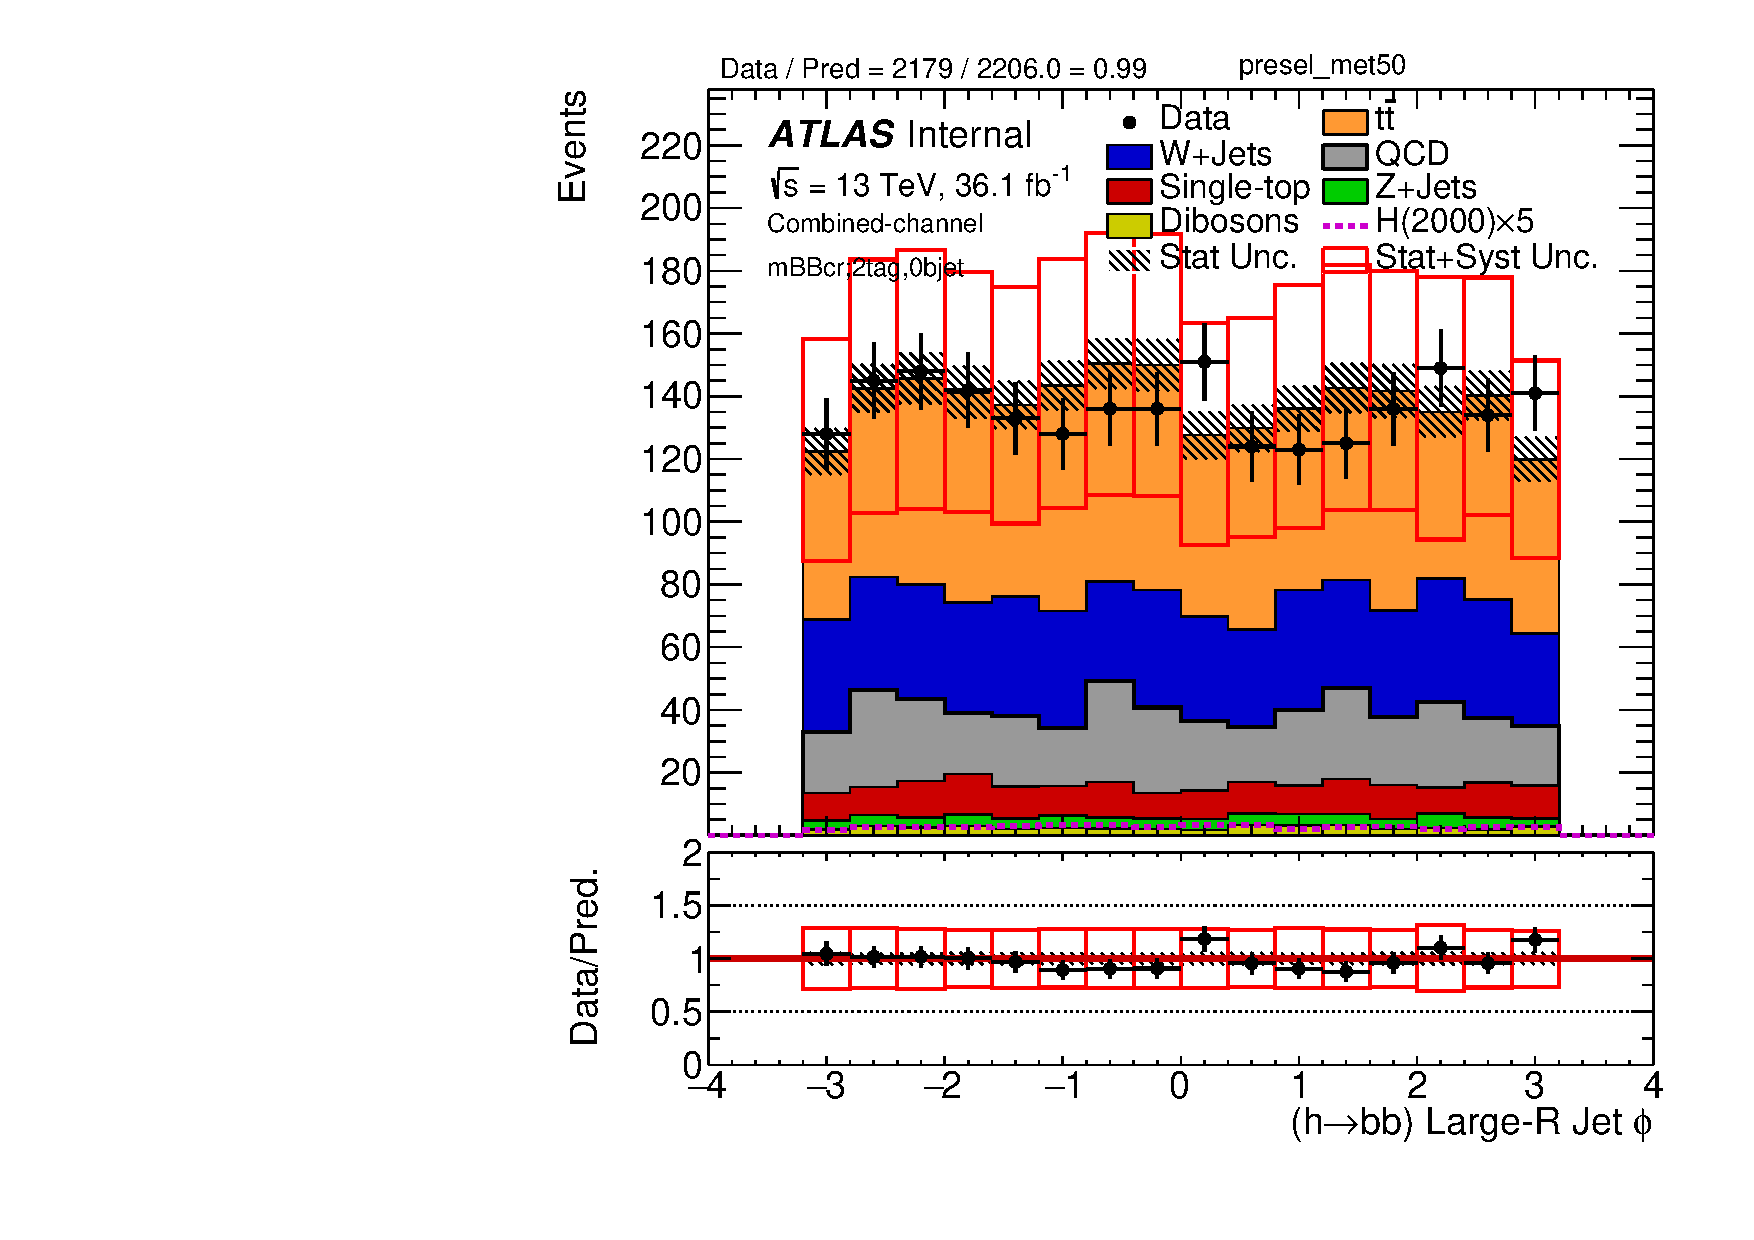
\includegraphics[scale=0.33]{./figures/boosted/PlotsInMbbCR/DataMC_2tag_0bjet_mbbcr_lepton_presel_met50_HbbPhi} 
\caption{Kinematic distributions of the reconstructed large-$R$ jet in the mBB control region (mBBcr).}
\label{fig:boosted_mbbcr_largerjet}
\end{center}
\end{figure}
 
\begin{figure}[!h]
\begin{center}
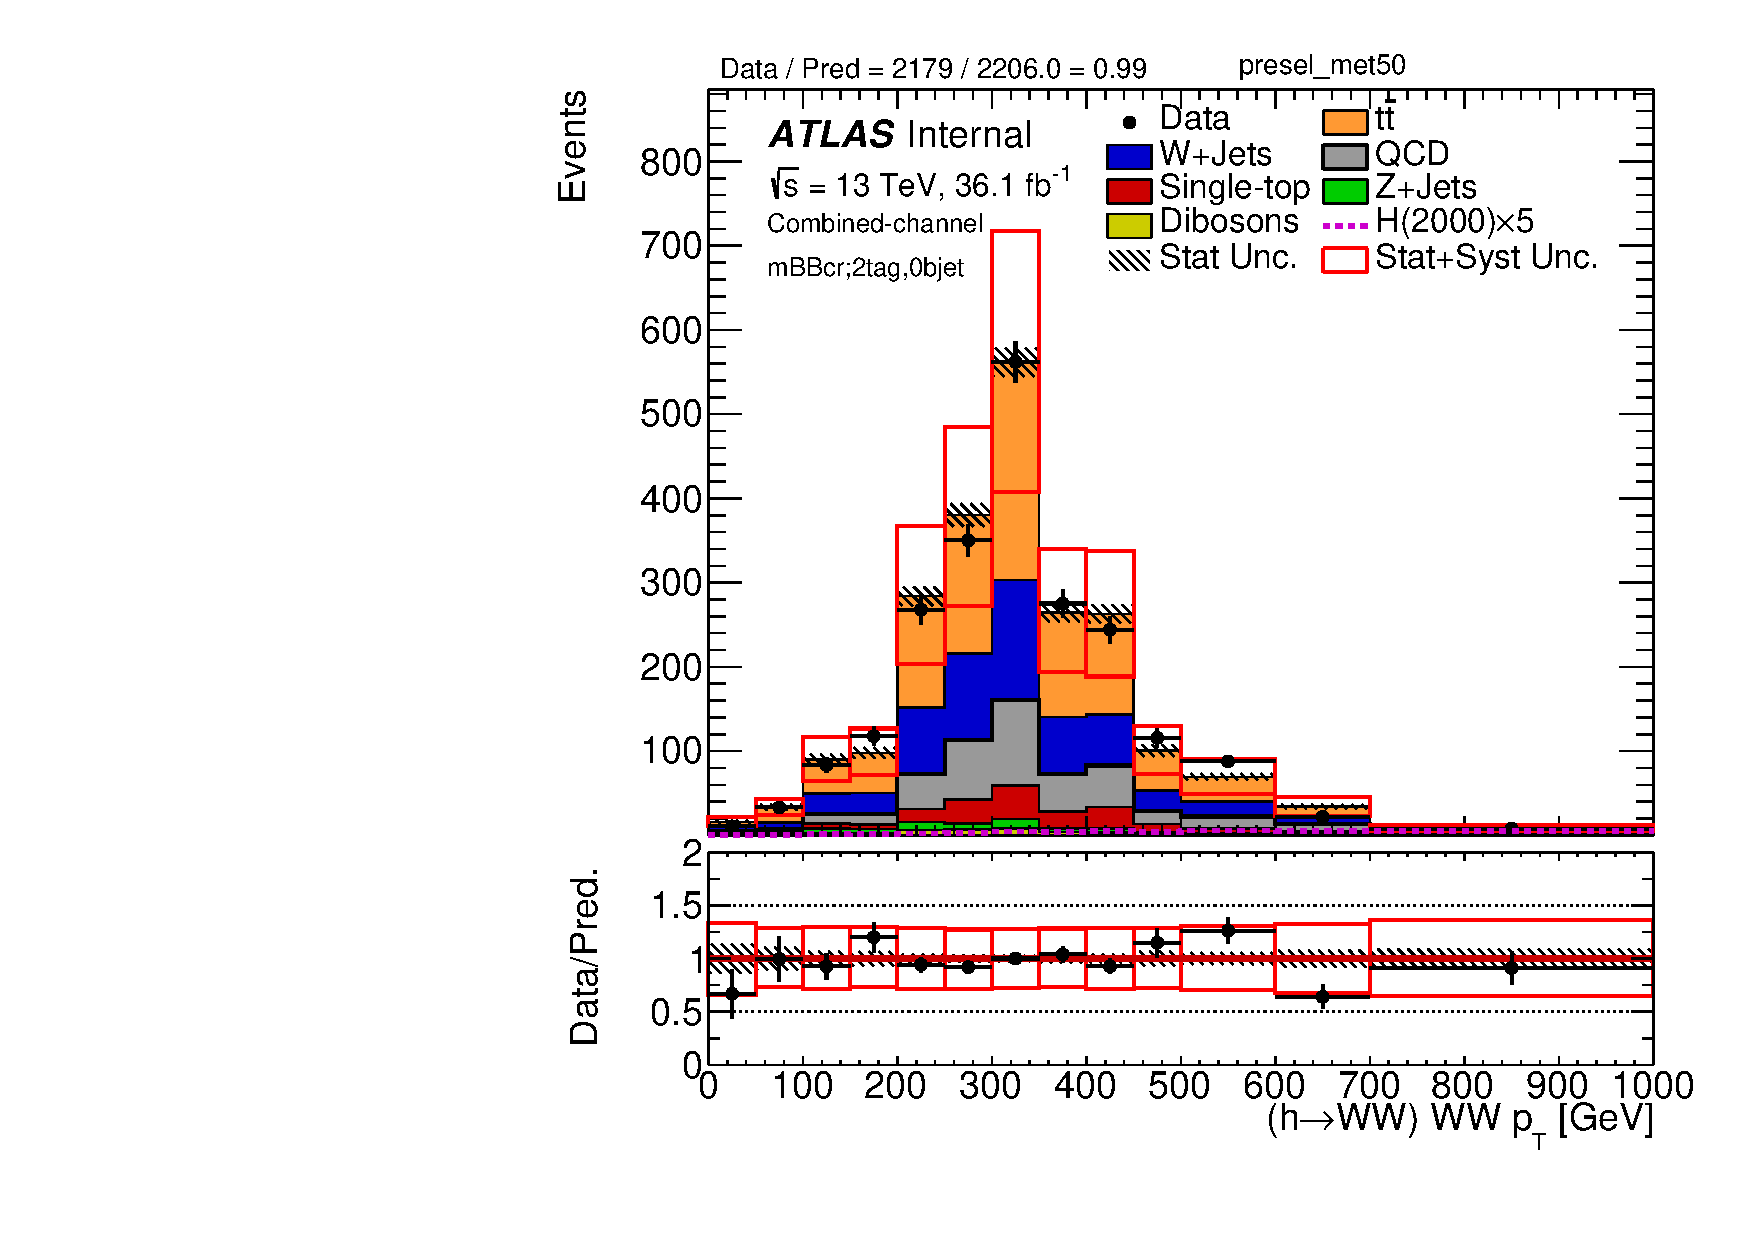
\includegraphics[scale=0.33]{./figures/boosted/PlotsInMbbCR/DataMC_2tag_0bjet_mbbcr_lepton_presel_met50_WWPt}
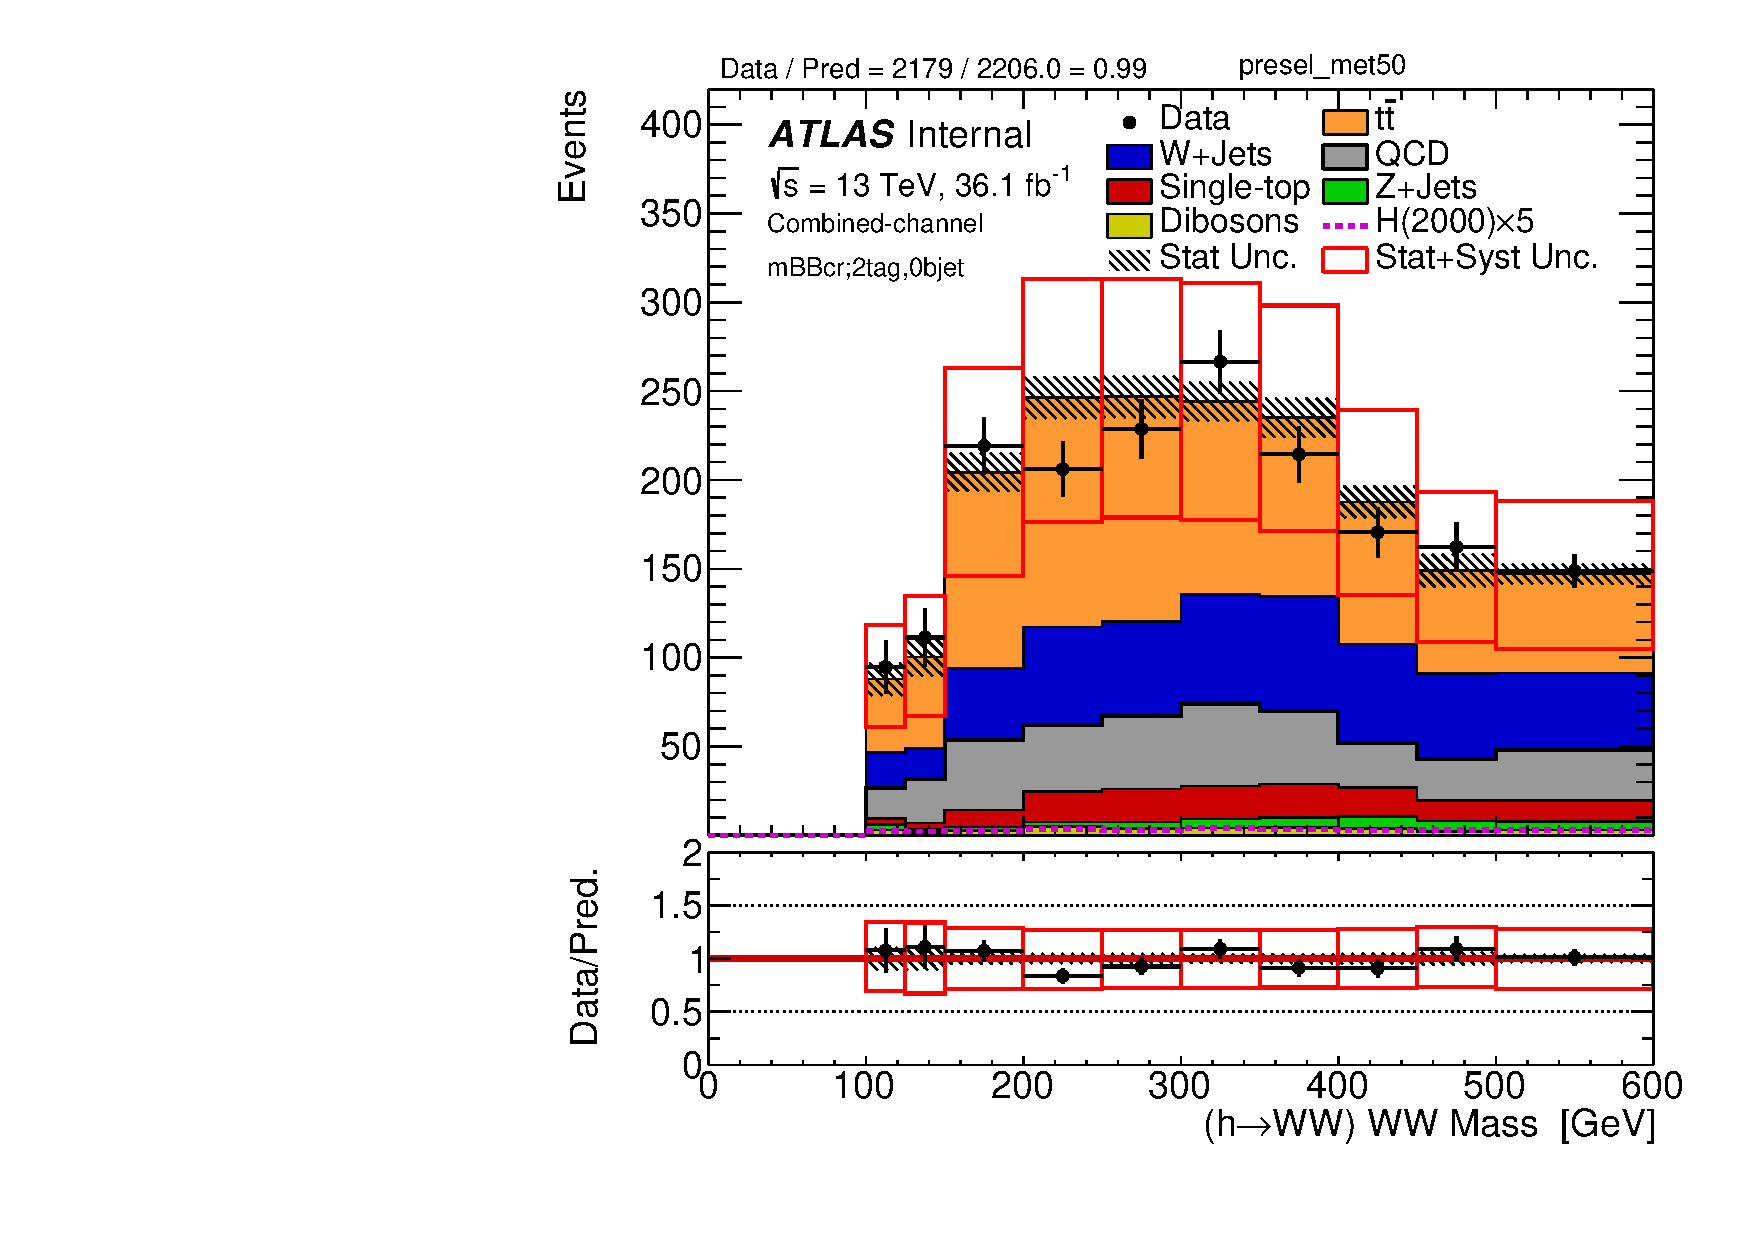
\includegraphics[scale=0.33]{./figures/boosted/PlotsInMbbCR/DataMC_2tag_0bjet_mbbcr_lepton_presel_met50_WWMass} \\
\par\medskip
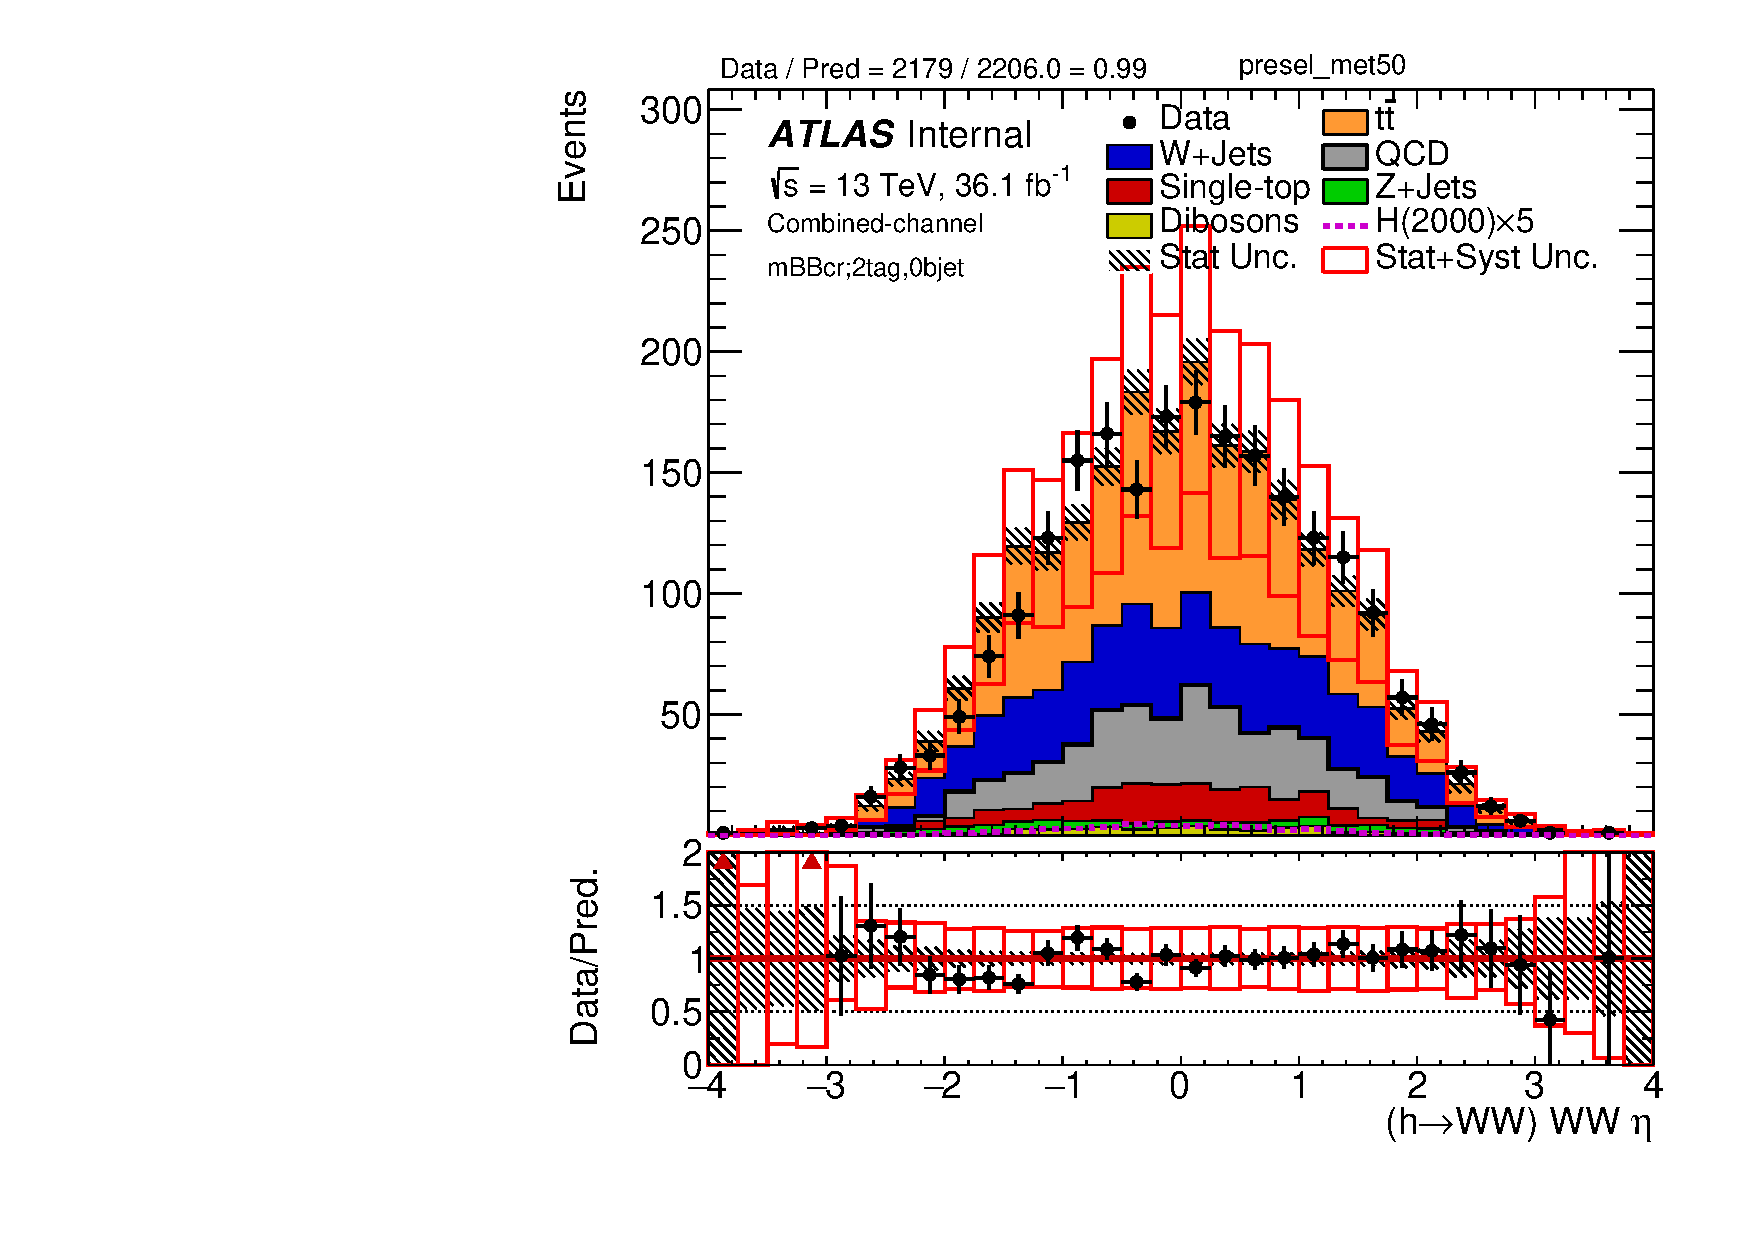
\includegraphics[scale=0.33]{./figures/boosted/PlotsInMbbCR/DataMC_2tag_0bjet_mbbcr_lepton_presel_met50_WWEta}
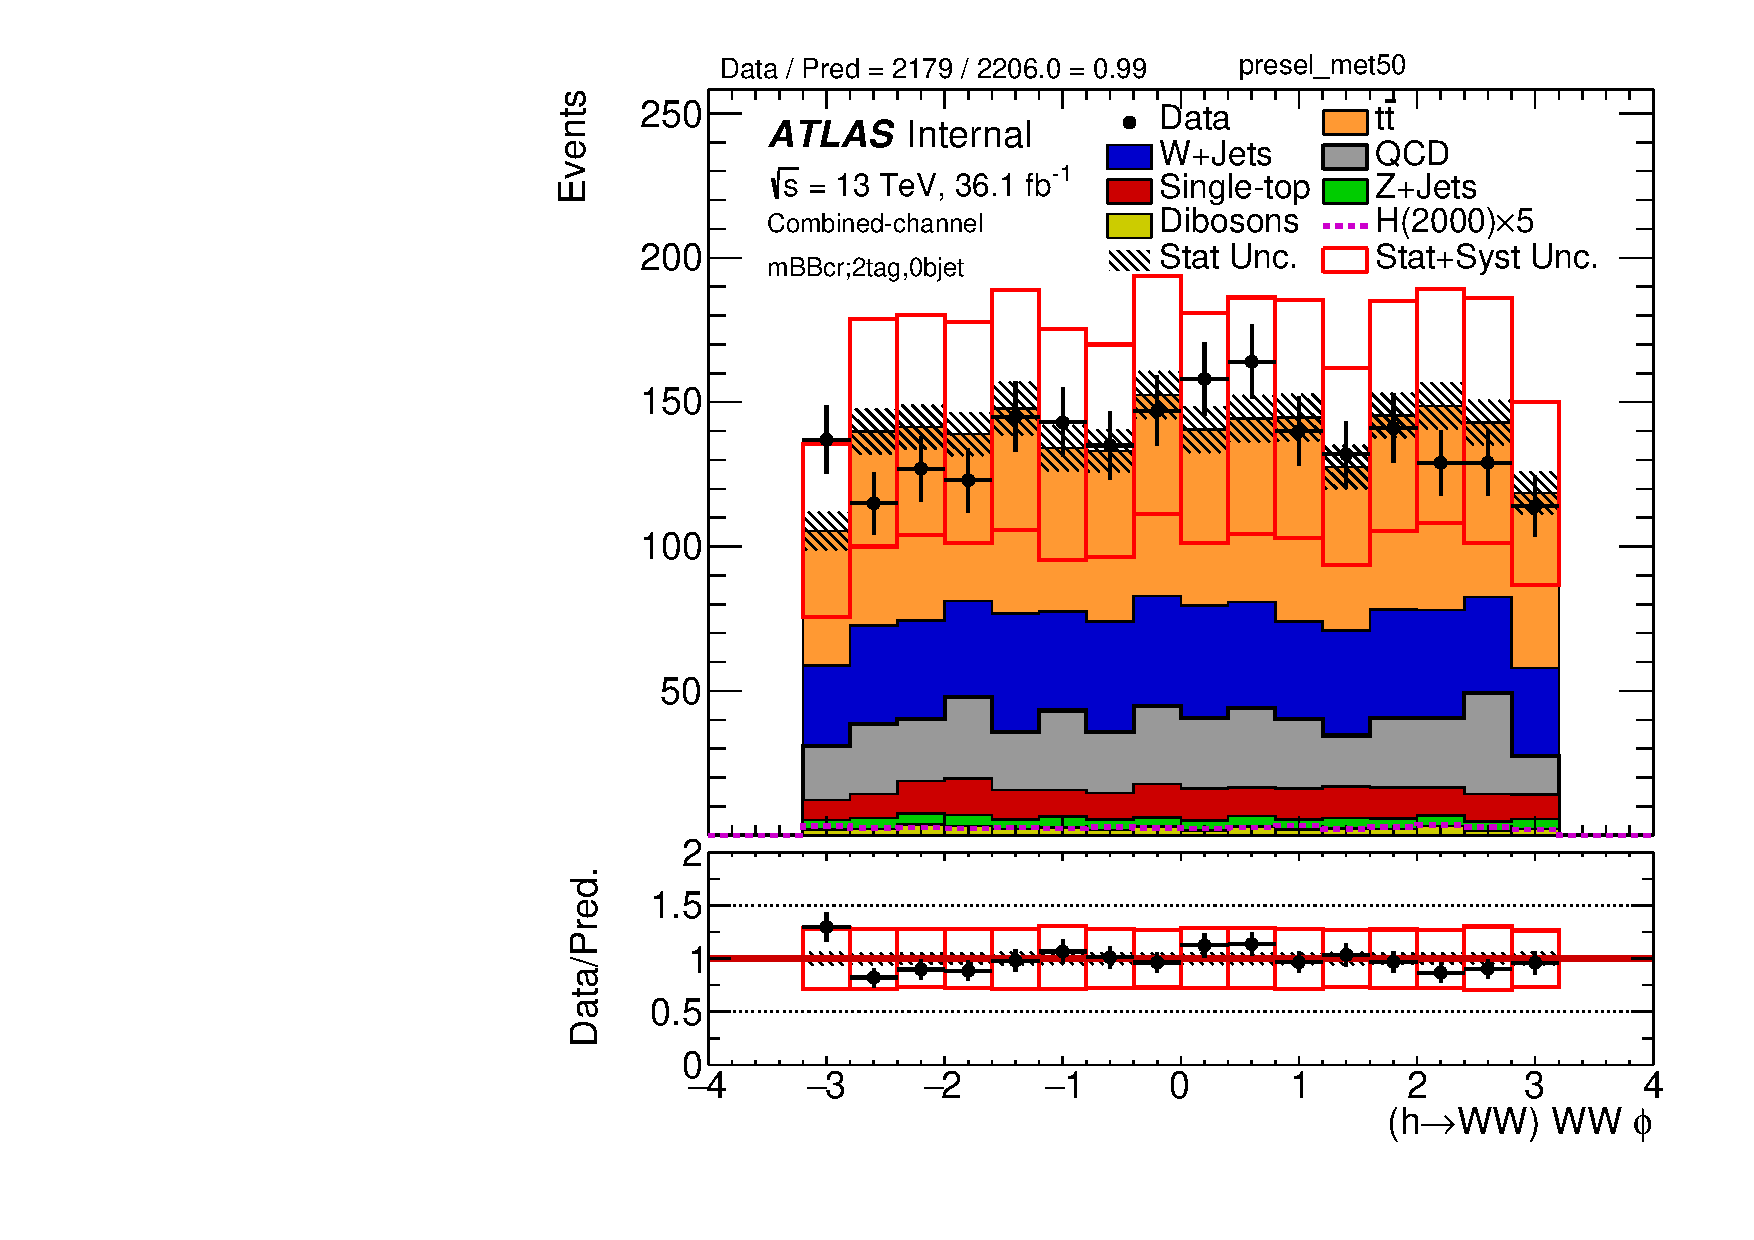
\includegraphics[scale=0.33]{./figures/boosted/PlotsInMbbCR/DataMC_2tag_0bjet_mbbcr_lepton_presel_met50_WWPhi}
\caption{Kinematic distributions of the reconstructed $h \to WW$ system in the mBB control region (mBBcr).}
\label{fig:boosted_mbbcr_wwsystem}
\end{center}
\end{figure}
 
\begin{figure}[!h]
\begin{center}
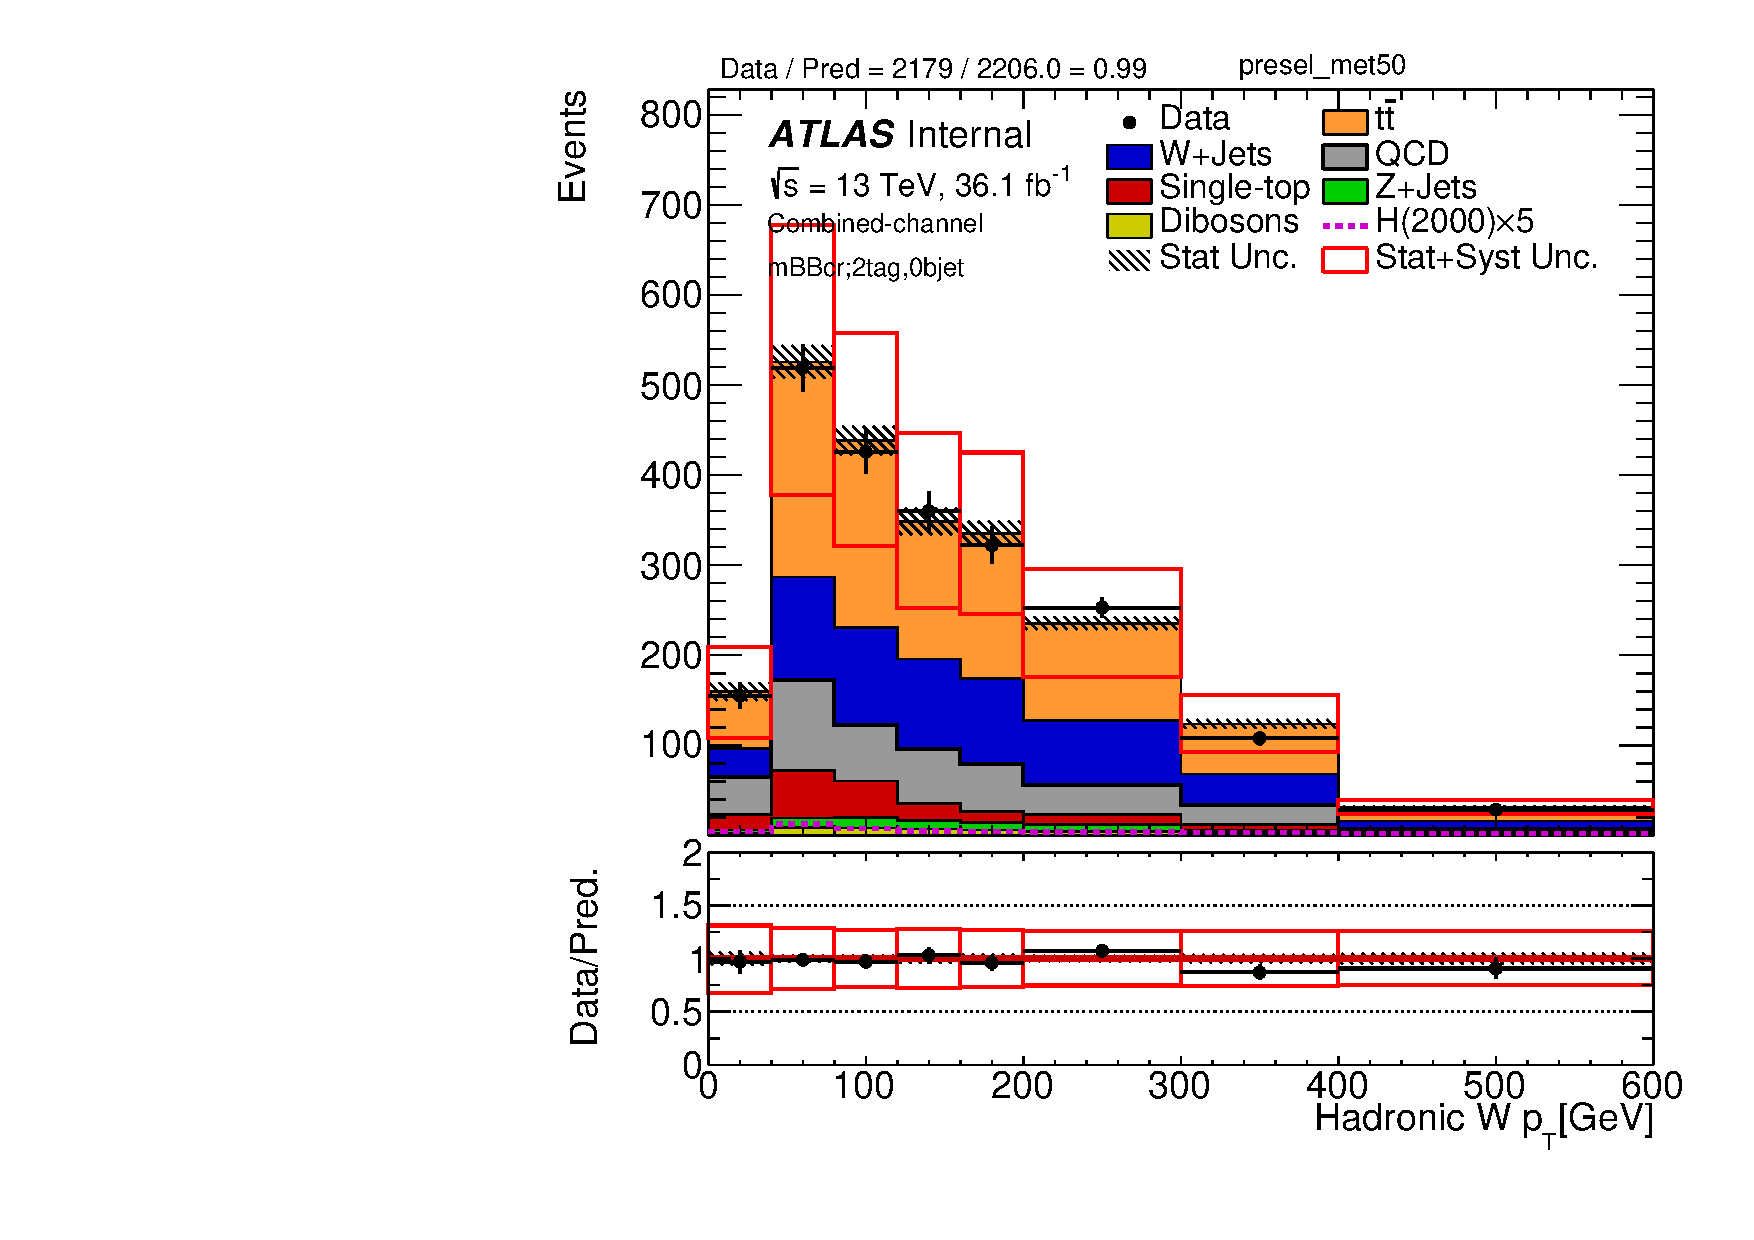
\includegraphics[scale=0.33]{./figures/boosted/PlotsInMbbCR/DataMC_2tag_0bjet_mbbcr_lepton_presel_met50_WhadPt}
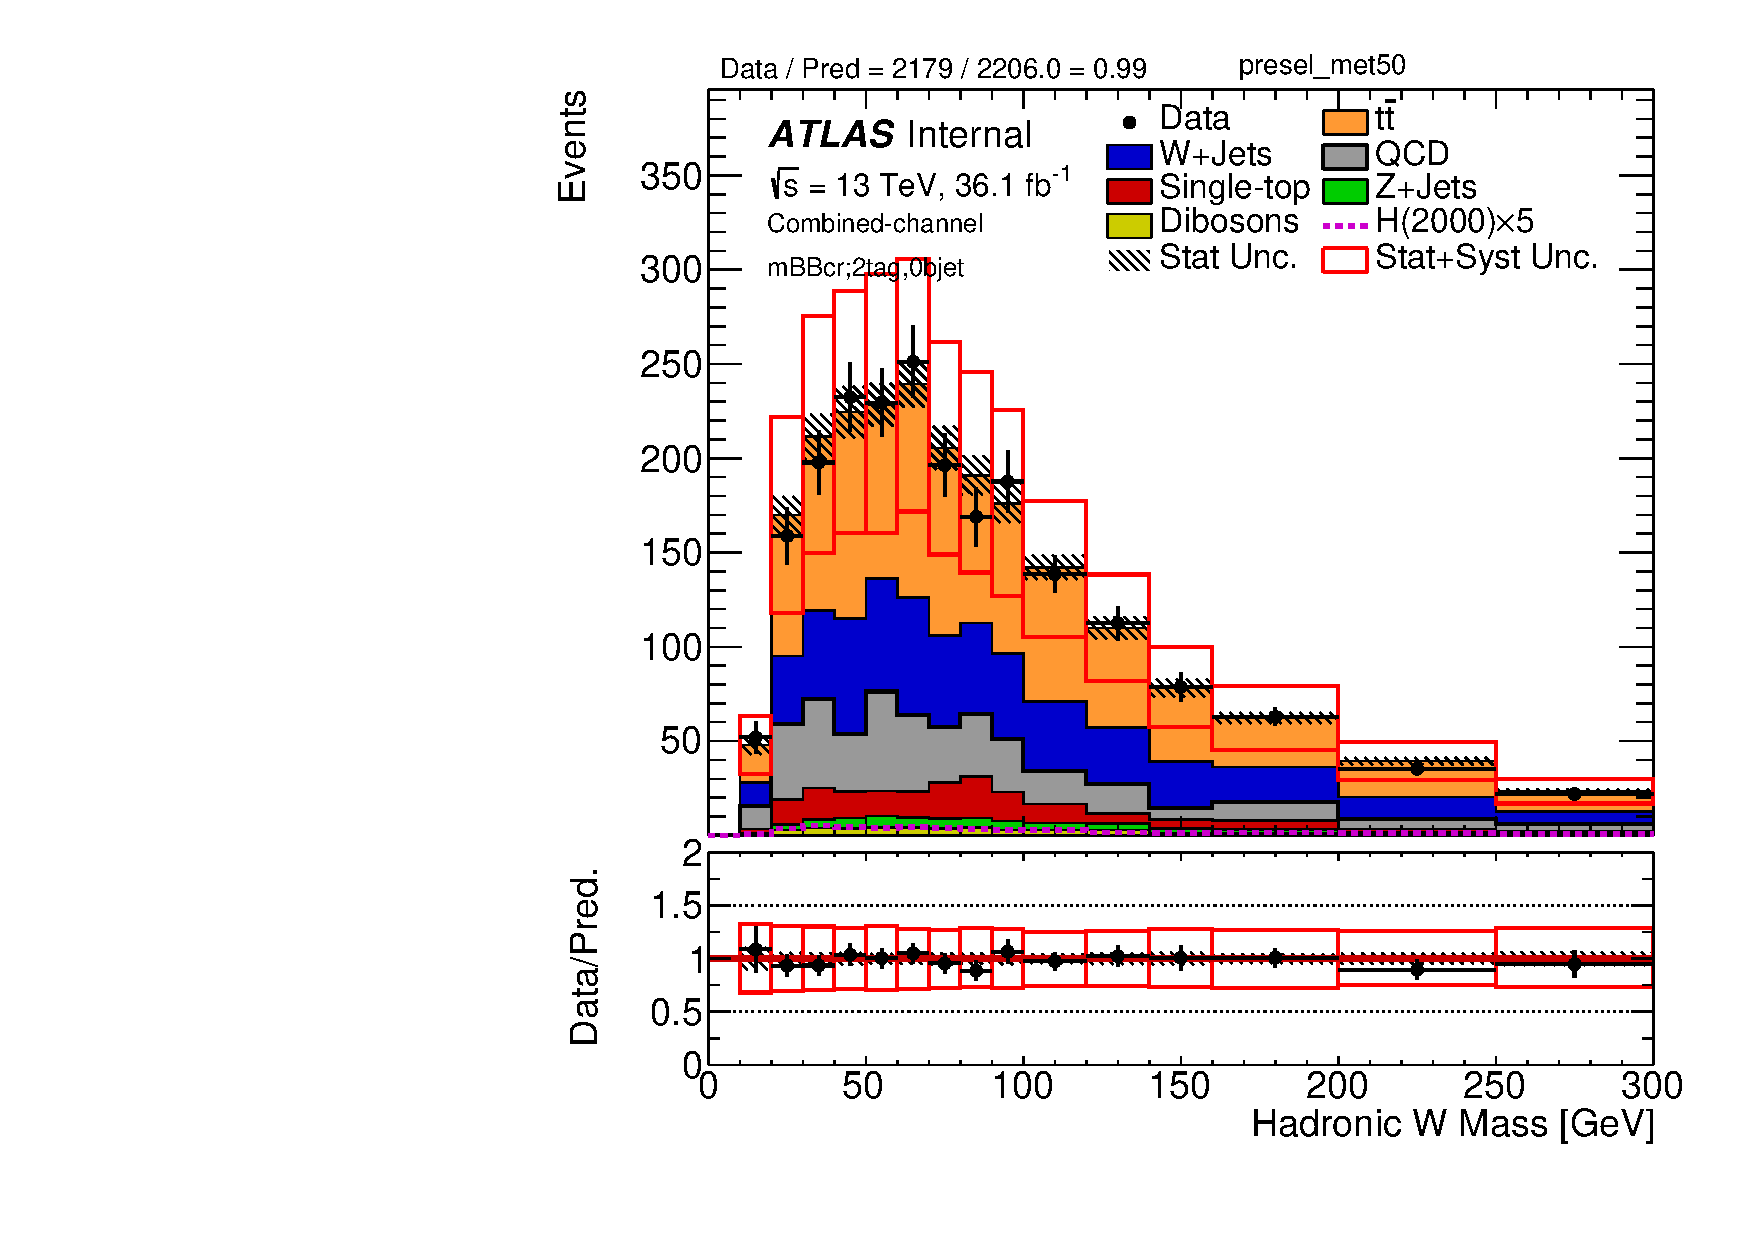
\includegraphics[scale=0.33]{./figures/boosted/PlotsInMbbCR/DataMC_2tag_0bjet_mbbcr_lepton_presel_met50_WhadMass} \\
\par\medskip
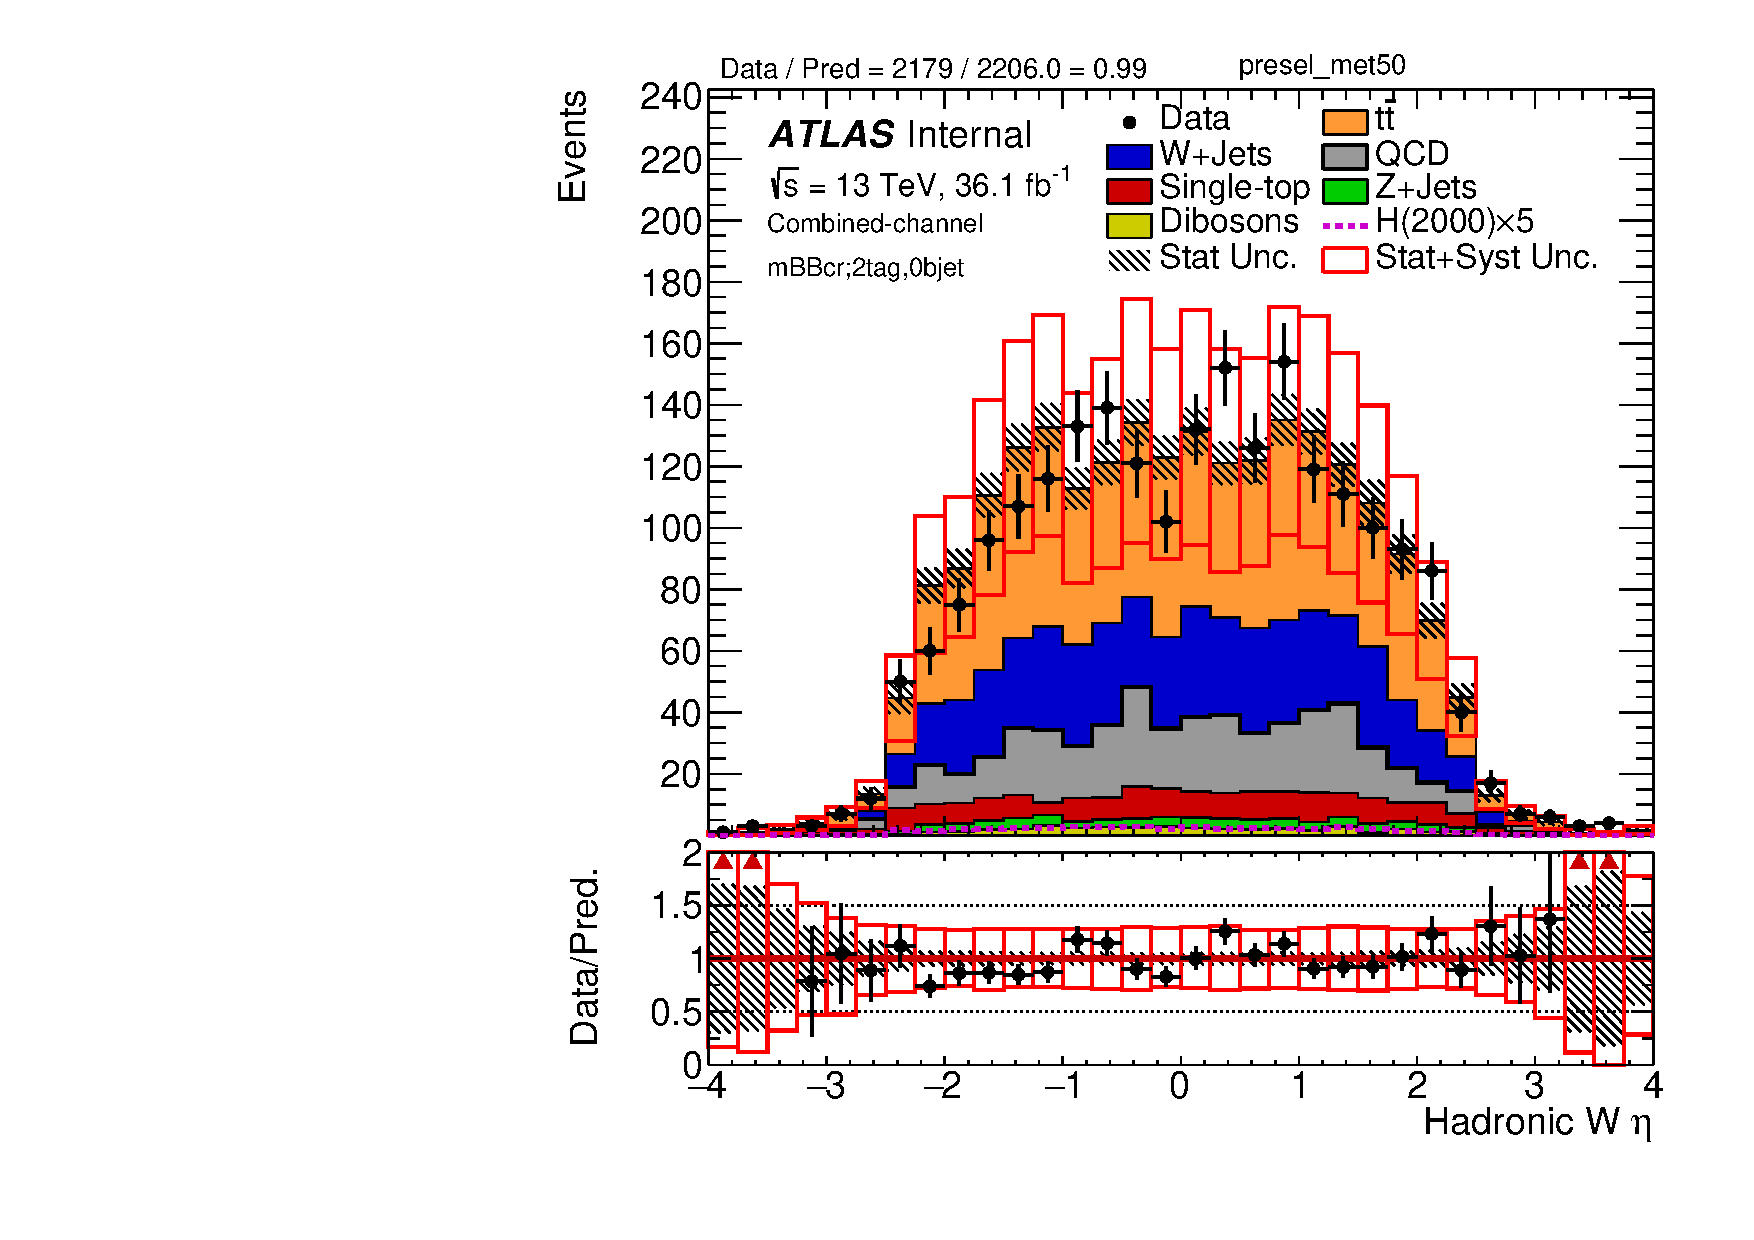
\includegraphics[scale=0.33]{./figures/boosted/PlotsInMbbCR/DataMC_2tag_0bjet_mbbcr_lepton_presel_met50_WhadEta}
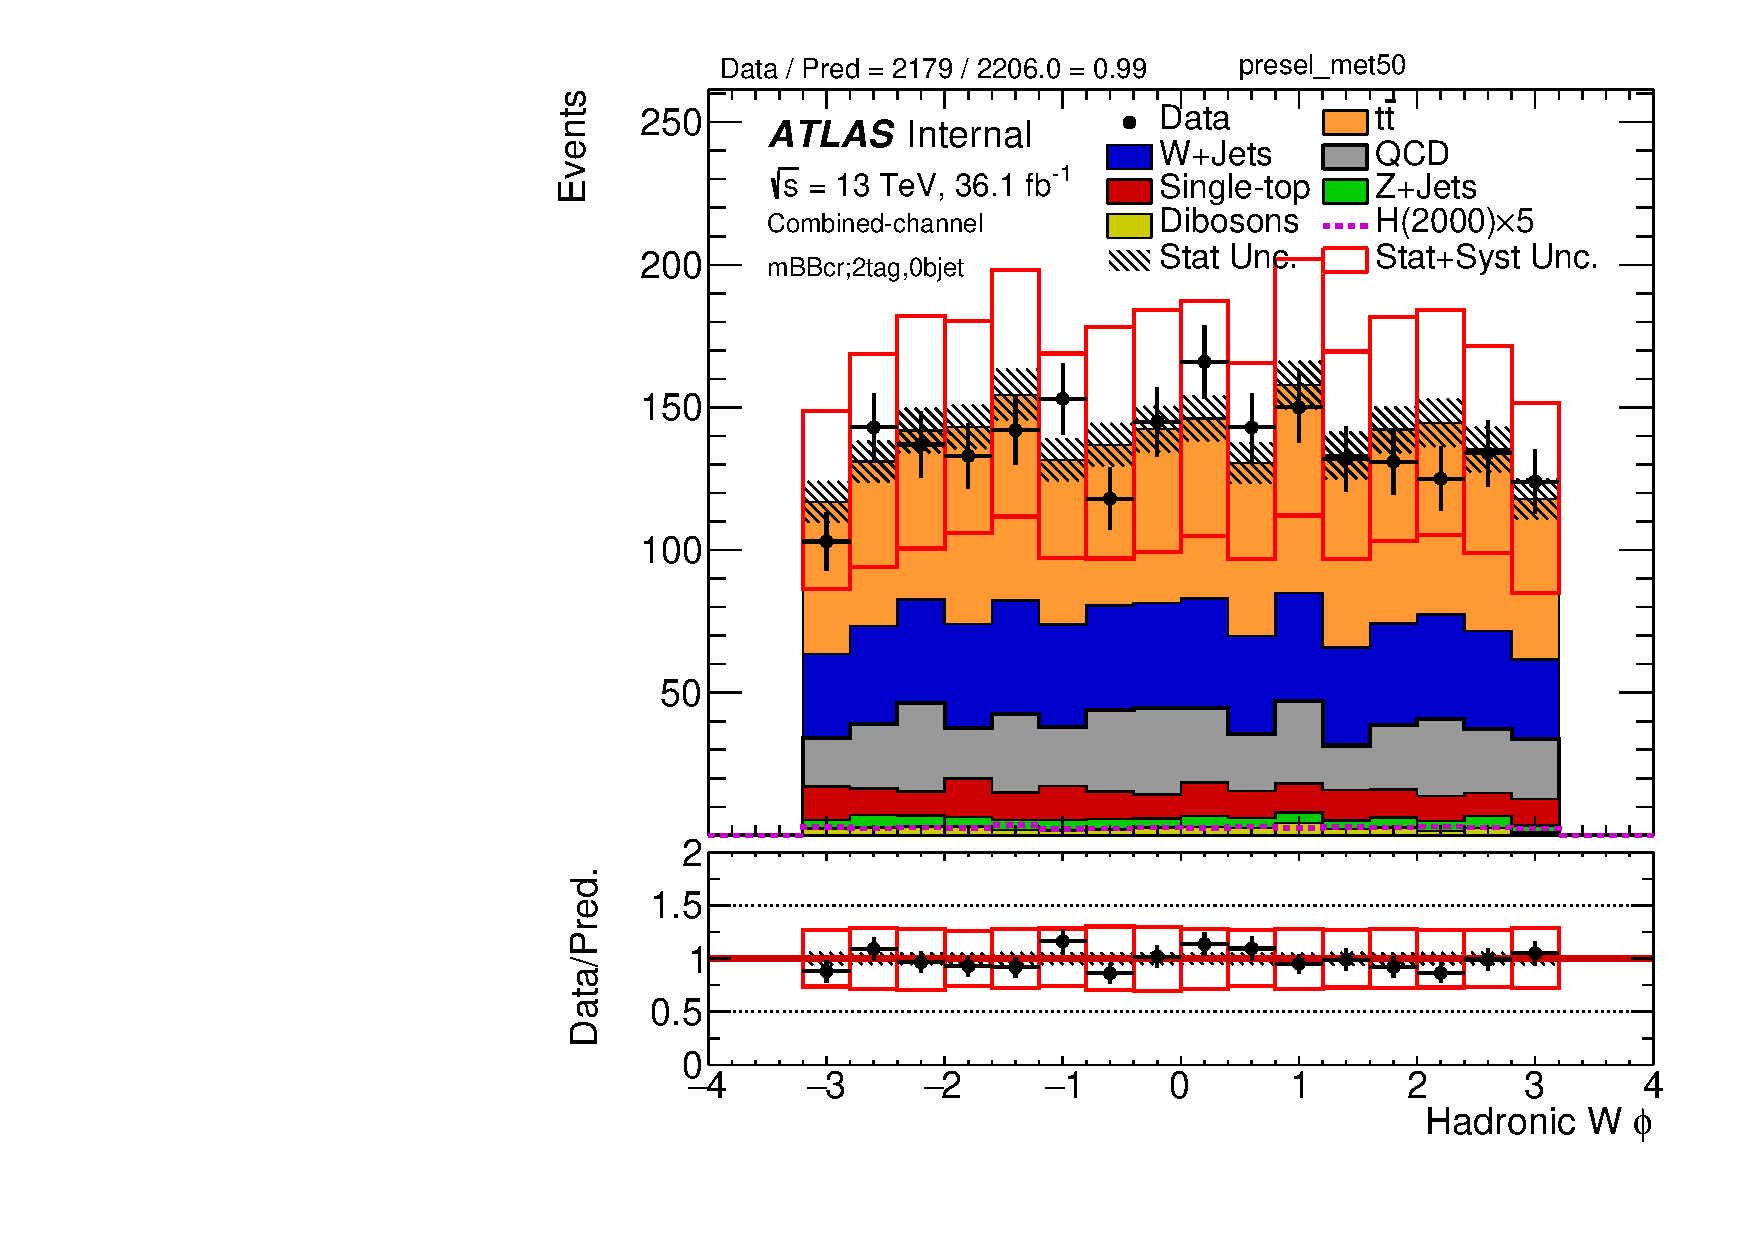
\includegraphics[scale=0.33]{./figures/boosted/PlotsInMbbCR/DataMC_2tag_0bjet_mbbcr_lepton_presel_met50_WhadPhi}
\caption{Kinematic distributions of the reconstructed $W \to q\bar{q}$ system in the mBB control region (mBBcr).}
\label{fig:boosted_mbbcr_whad}
\end{center}
\end{figure}
 
\begin{figure}[!h]
\begin{center}
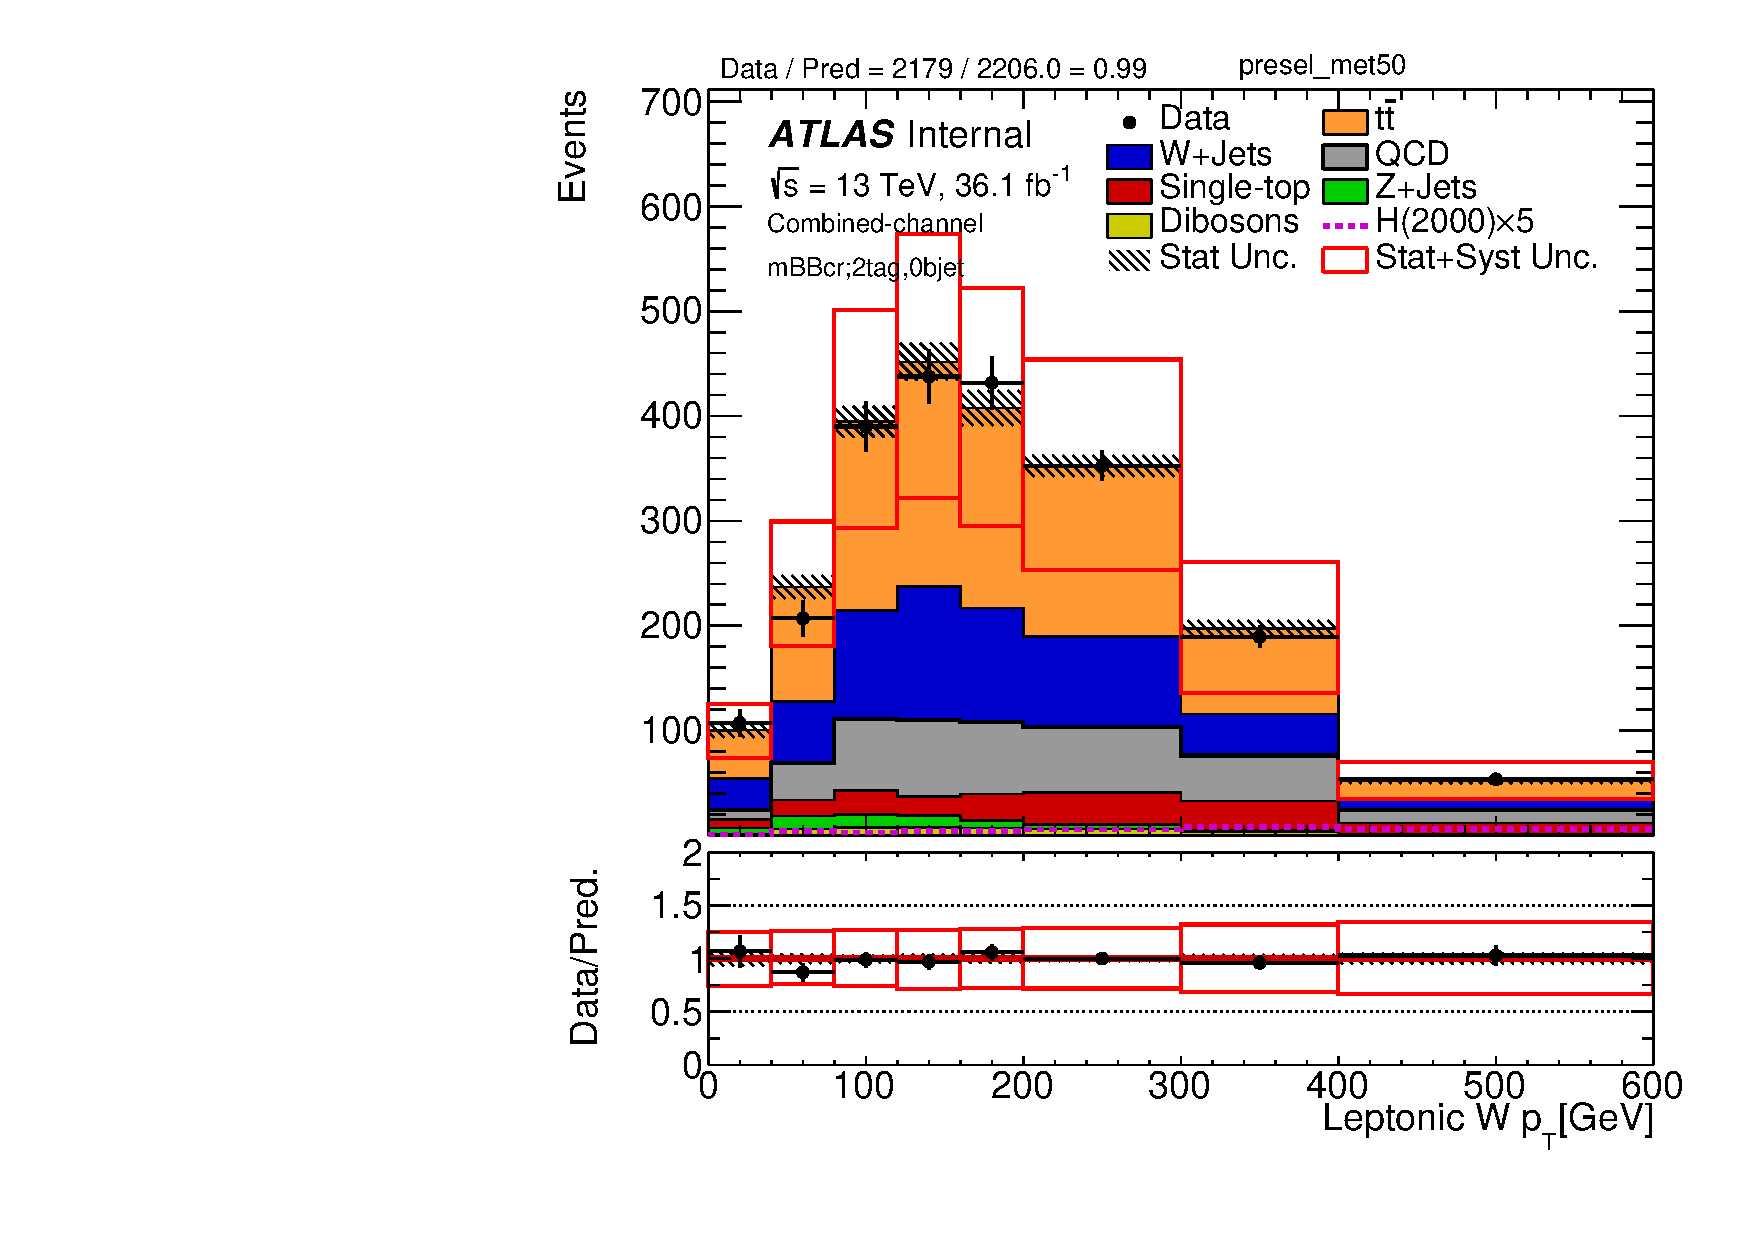
\includegraphics[scale=0.33]{./figures/boosted/PlotsInMbbCR/DataMC_2tag_0bjet_mbbcr_lepton_presel_met50_WlepPt}
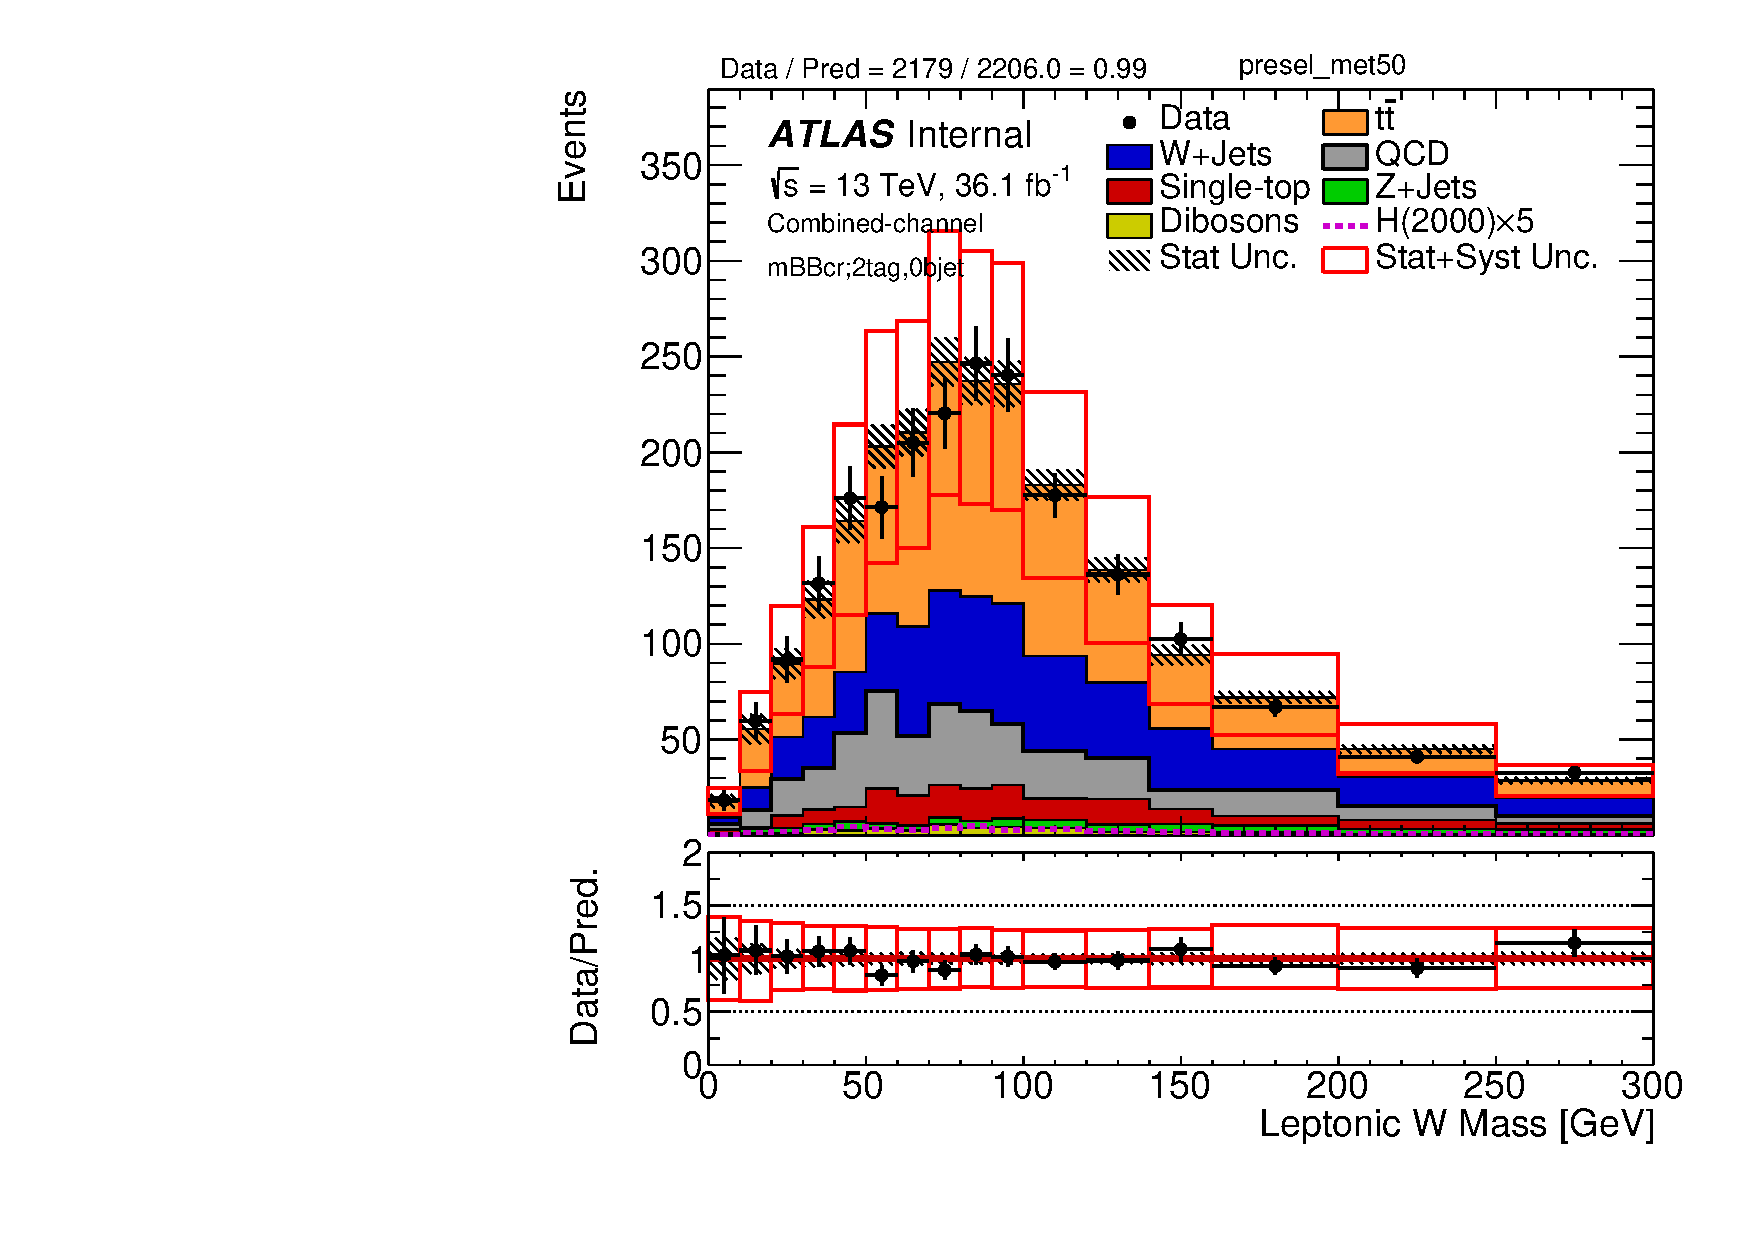
\includegraphics[scale=0.33]{./figures/boosted/PlotsInMbbCR/DataMC_2tag_0bjet_mbbcr_lepton_presel_met50_WlepMass} \\
\par\medskip
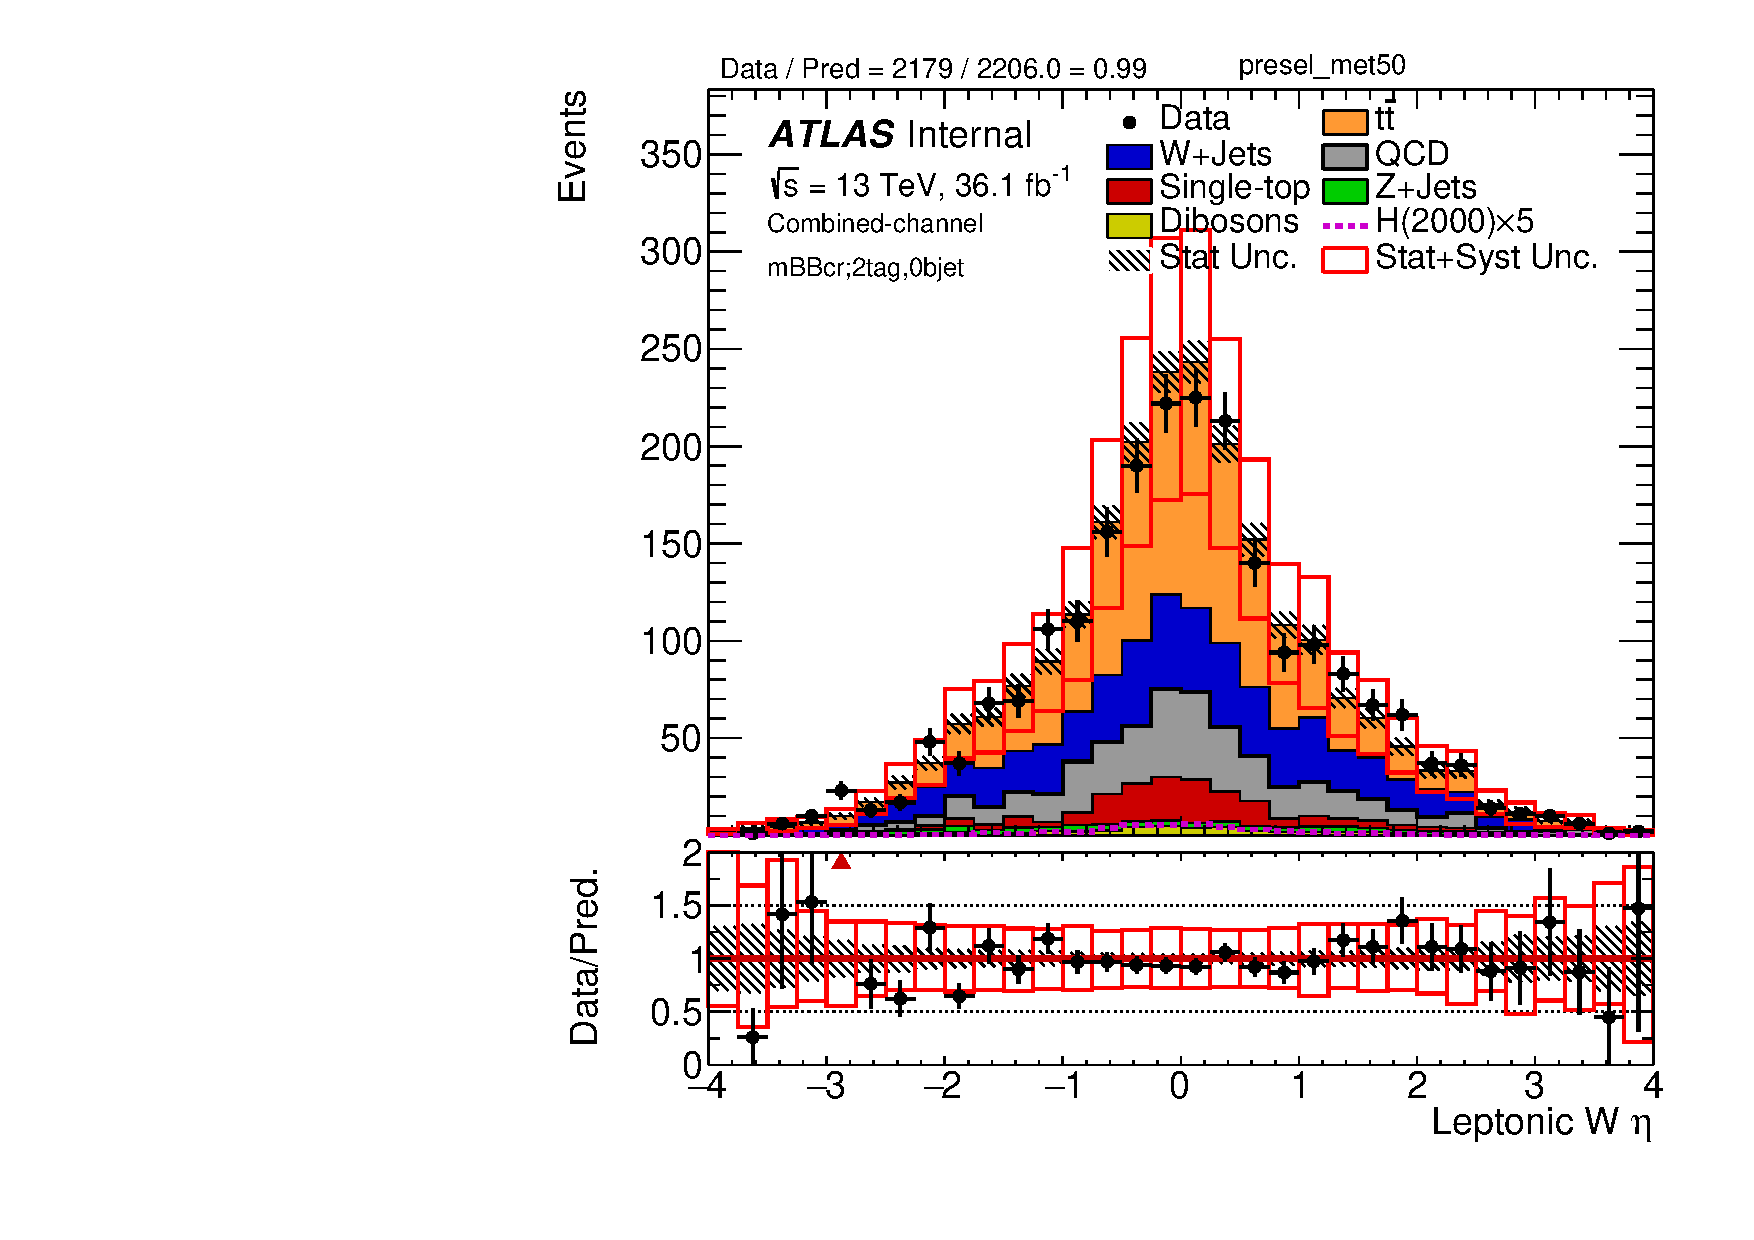
\includegraphics[scale=0.33]{./figures/boosted/PlotsInMbbCR/DataMC_2tag_0bjet_mbbcr_lepton_presel_met50_WlepEta}
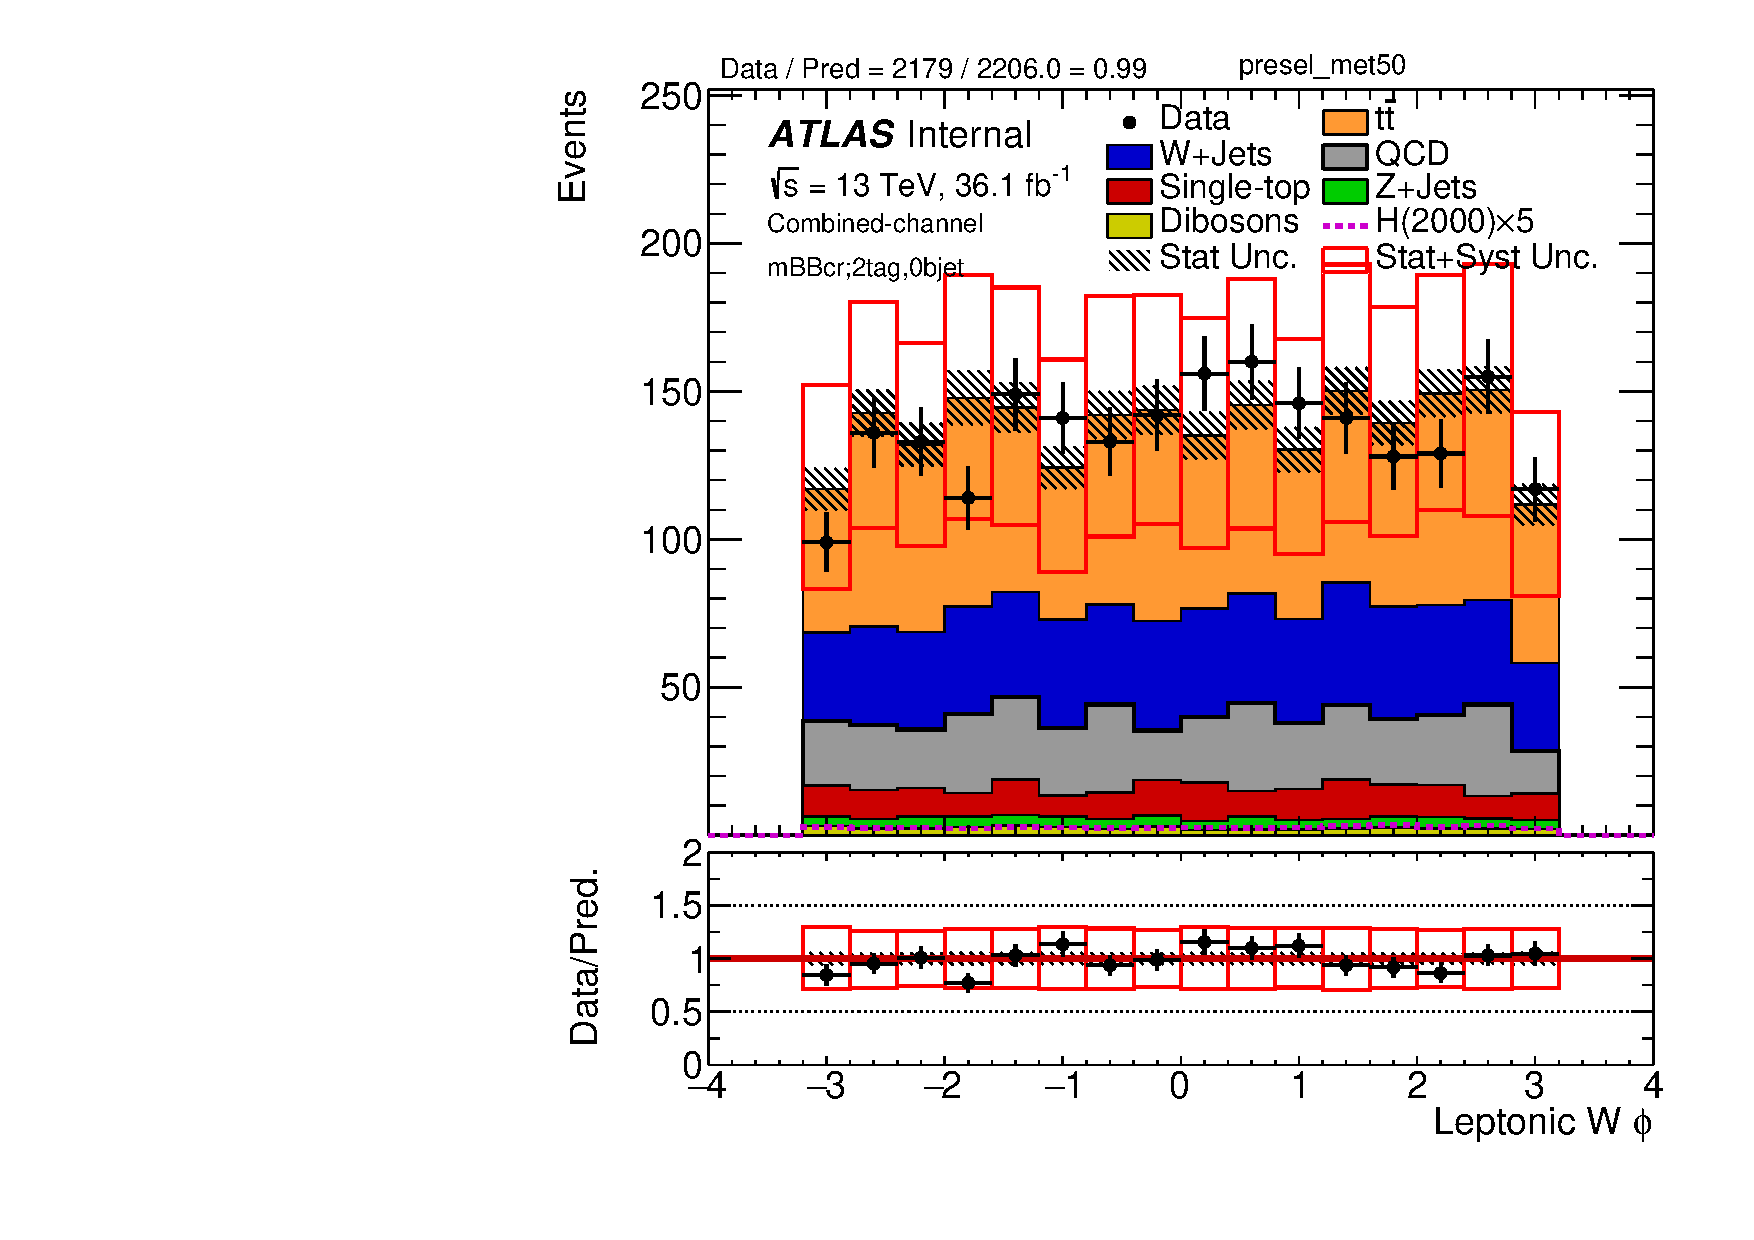
\includegraphics[scale=0.33]{./figures/boosted/PlotsInMbbCR/DataMC_2tag_0bjet_mbbcr_lepton_presel_met50_WlepPhi}
\caption{Kinematic distributions of the reconstructed $W \to l\nu$ system in the mBB control region (mBBcr).}
\label{fig:boosted_mbbcr_wlep}
\end{center}
\end{figure}
 
\begin{figure}[!h]
\begin{center}
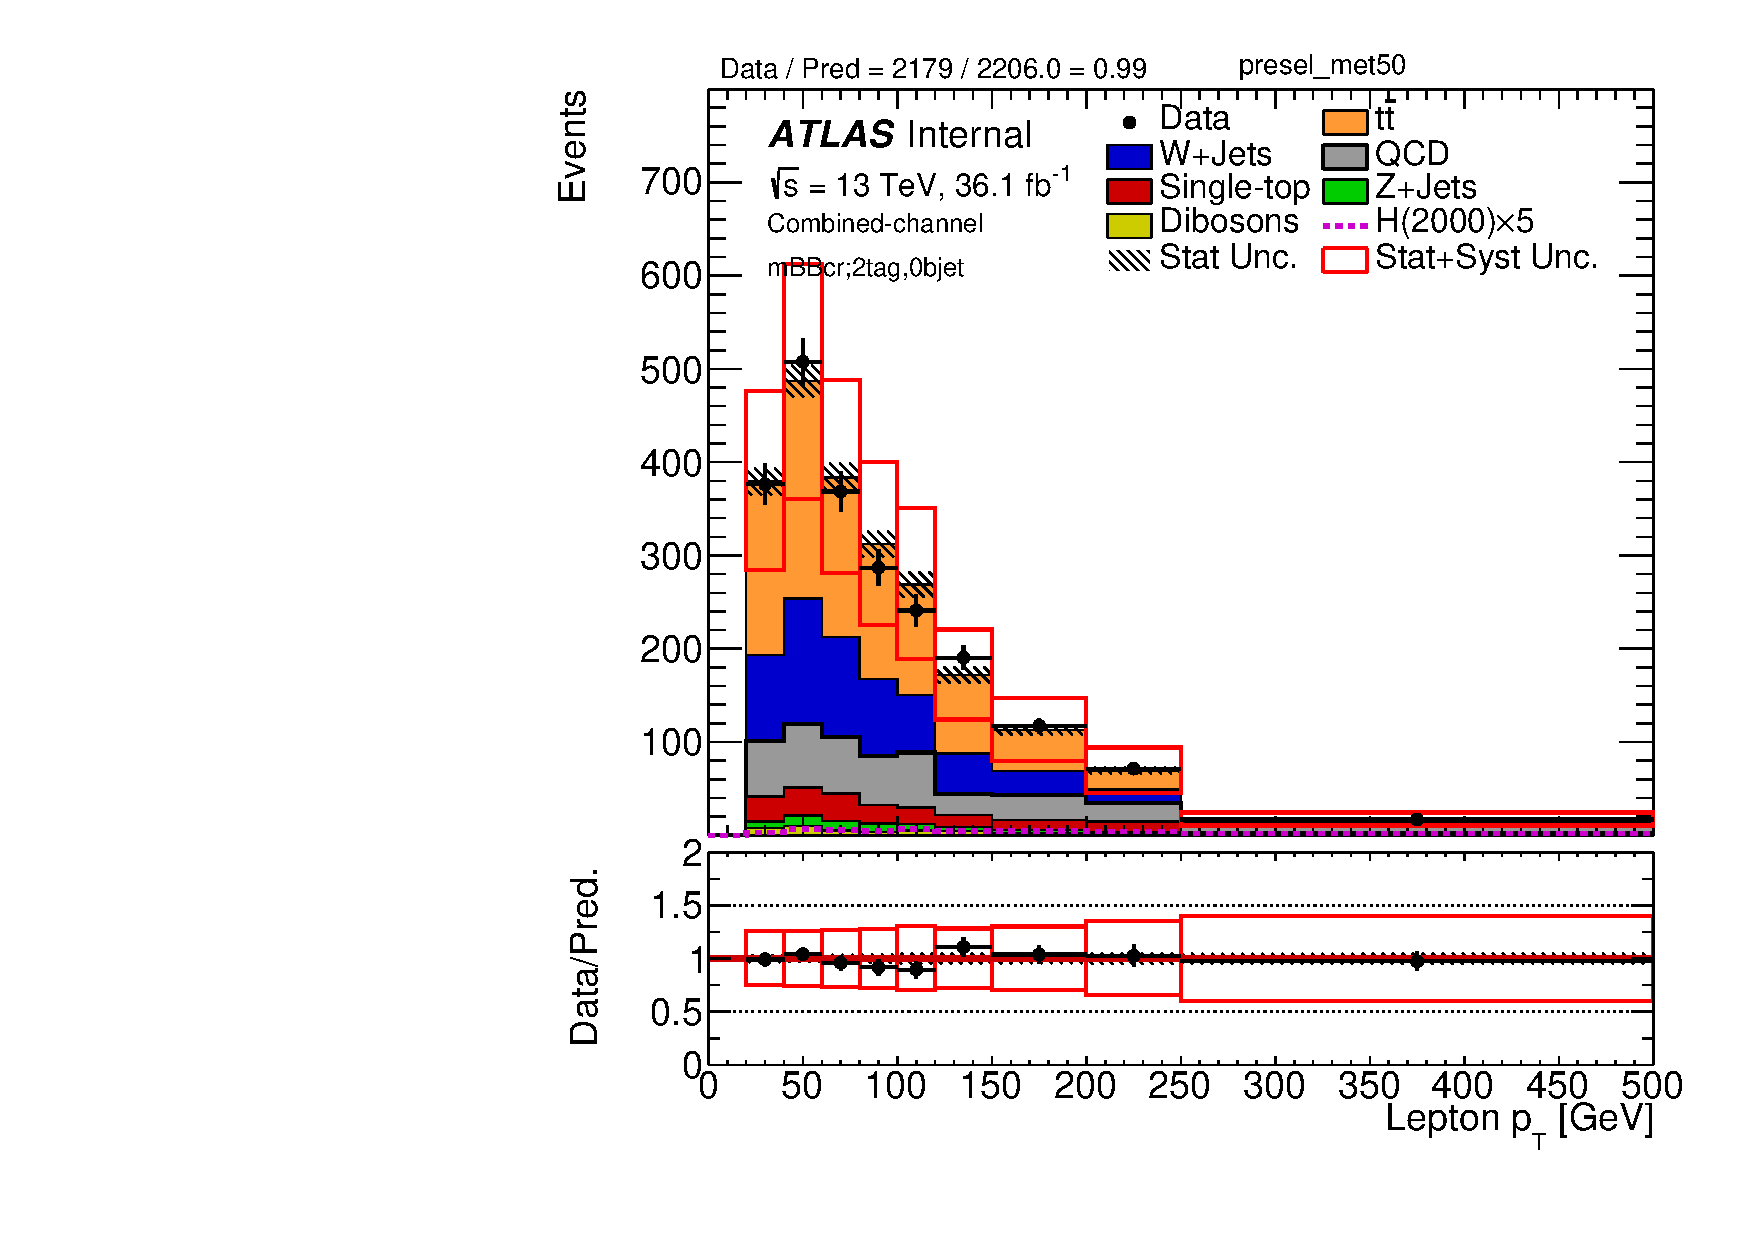
\includegraphics[scale=0.33]{./figures/boosted/PlotsInMbbCR/DataMC_2tag_0bjet_mbbcr_lepton_presel_met50_LepPt}
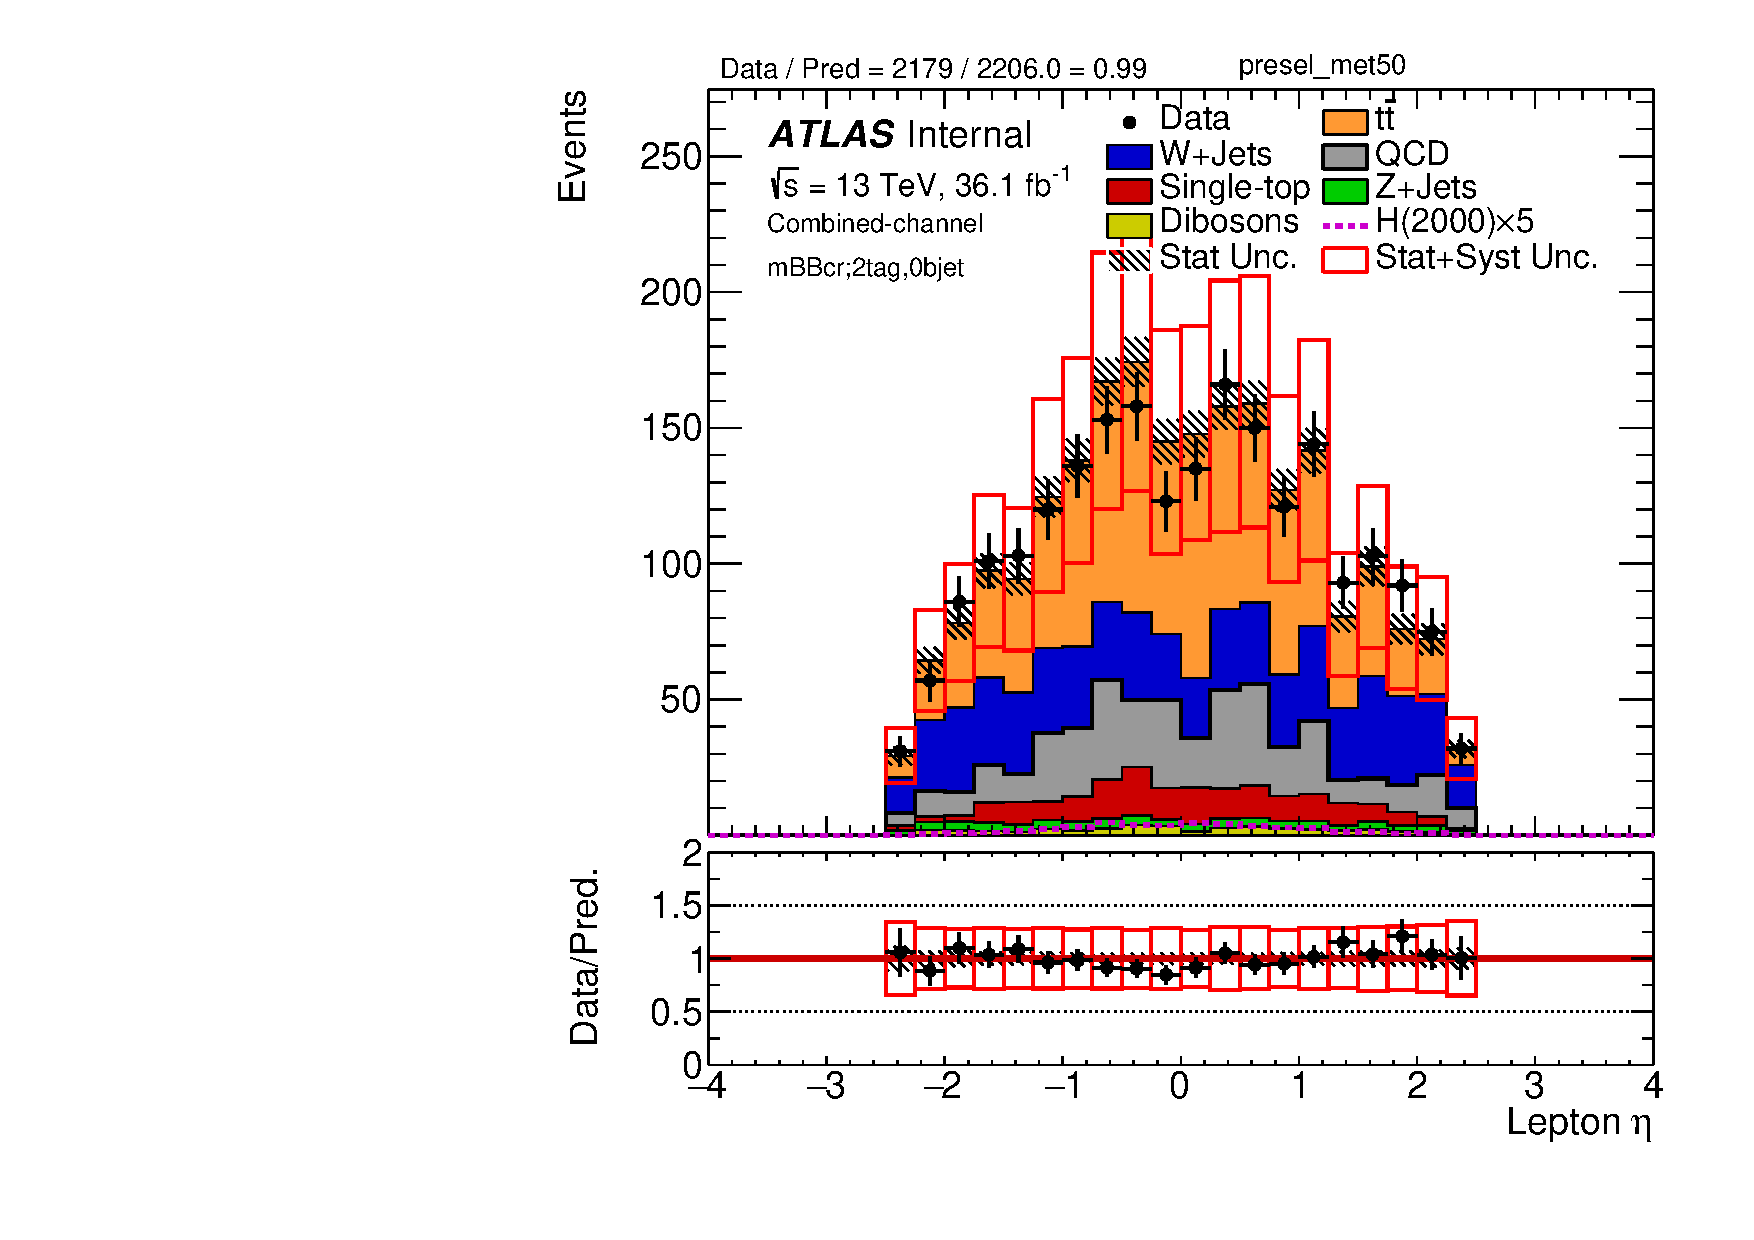
\includegraphics[scale=0.33]{./figures/boosted/PlotsInMbbCR/DataMC_2tag_0bjet_mbbcr_lepton_presel_met50_LepEta}\\
\par\medskip
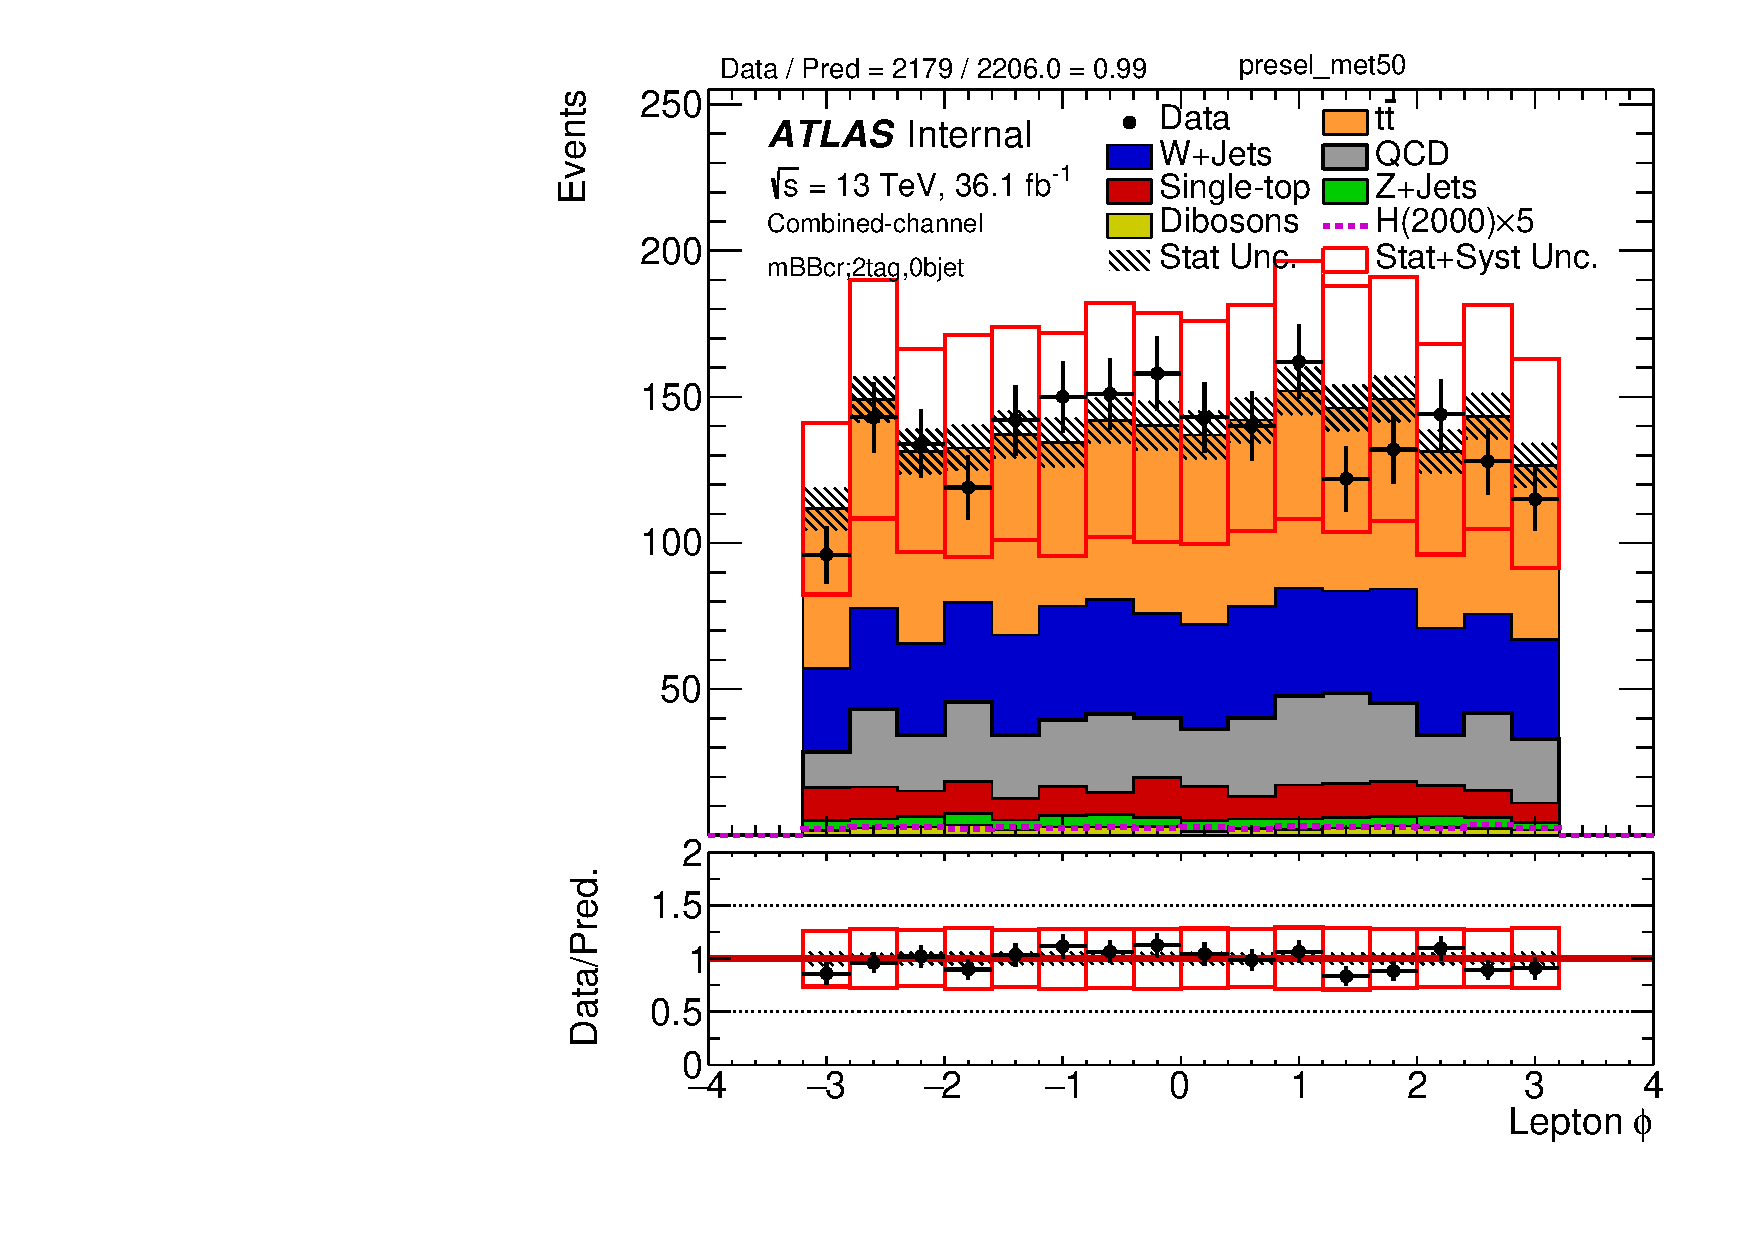
\includegraphics[scale=0.33]{./figures/boosted/PlotsInMbbCR/DataMC_2tag_0bjet_mbbcr_lepton_presel_met50_LepPhi}
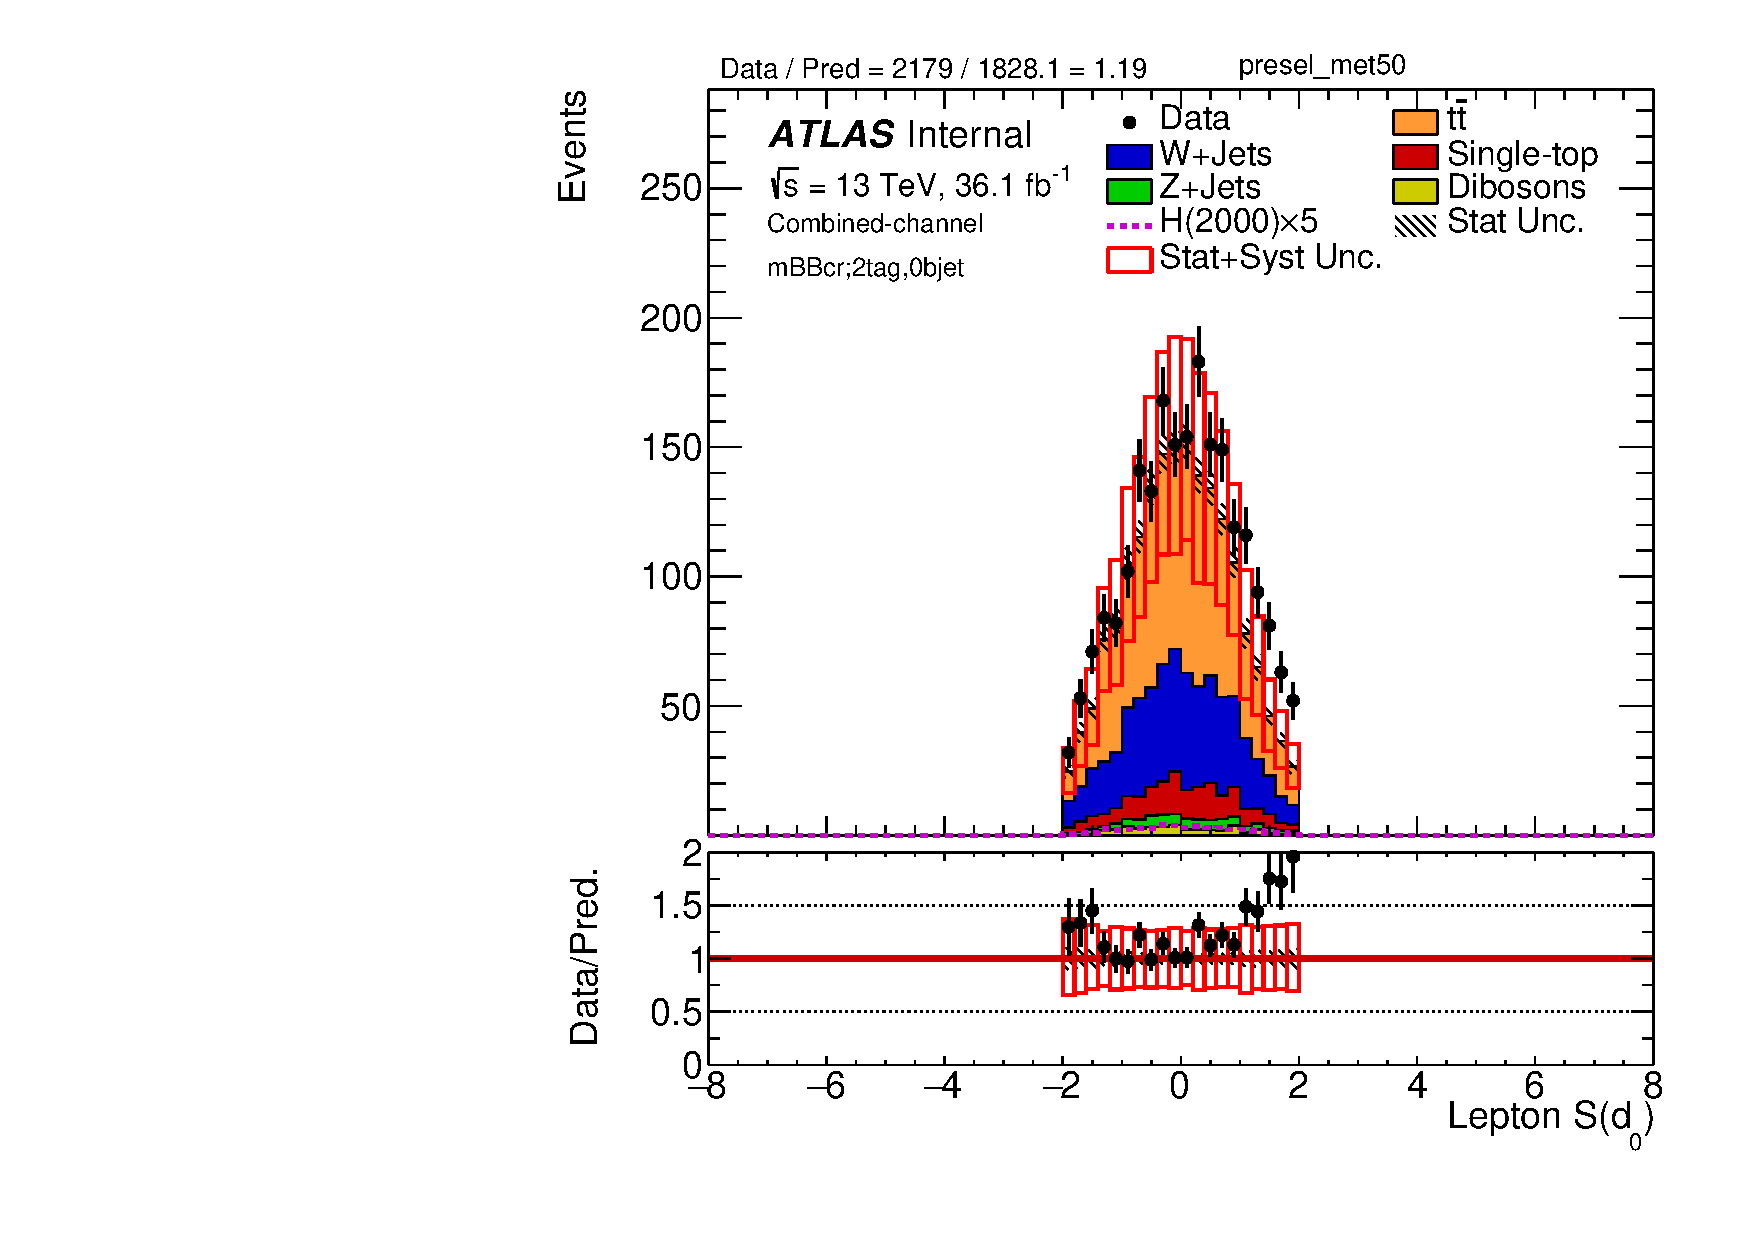
\includegraphics[scale=0.33]{./figures/boosted/PlotsInMbbCR/DataMC_2tag_0bjet_mbbcr_lepton_presel_met50_Lep_d0sigL}
\caption{Kinematic distributions of the selected lepton in the mBB control region (mBBcr).}
\label{fig:boosted_mbbcr_lepton}
\end{center}
\end{figure}
 
 
\begin{figure}[!ht]
\begin{center}
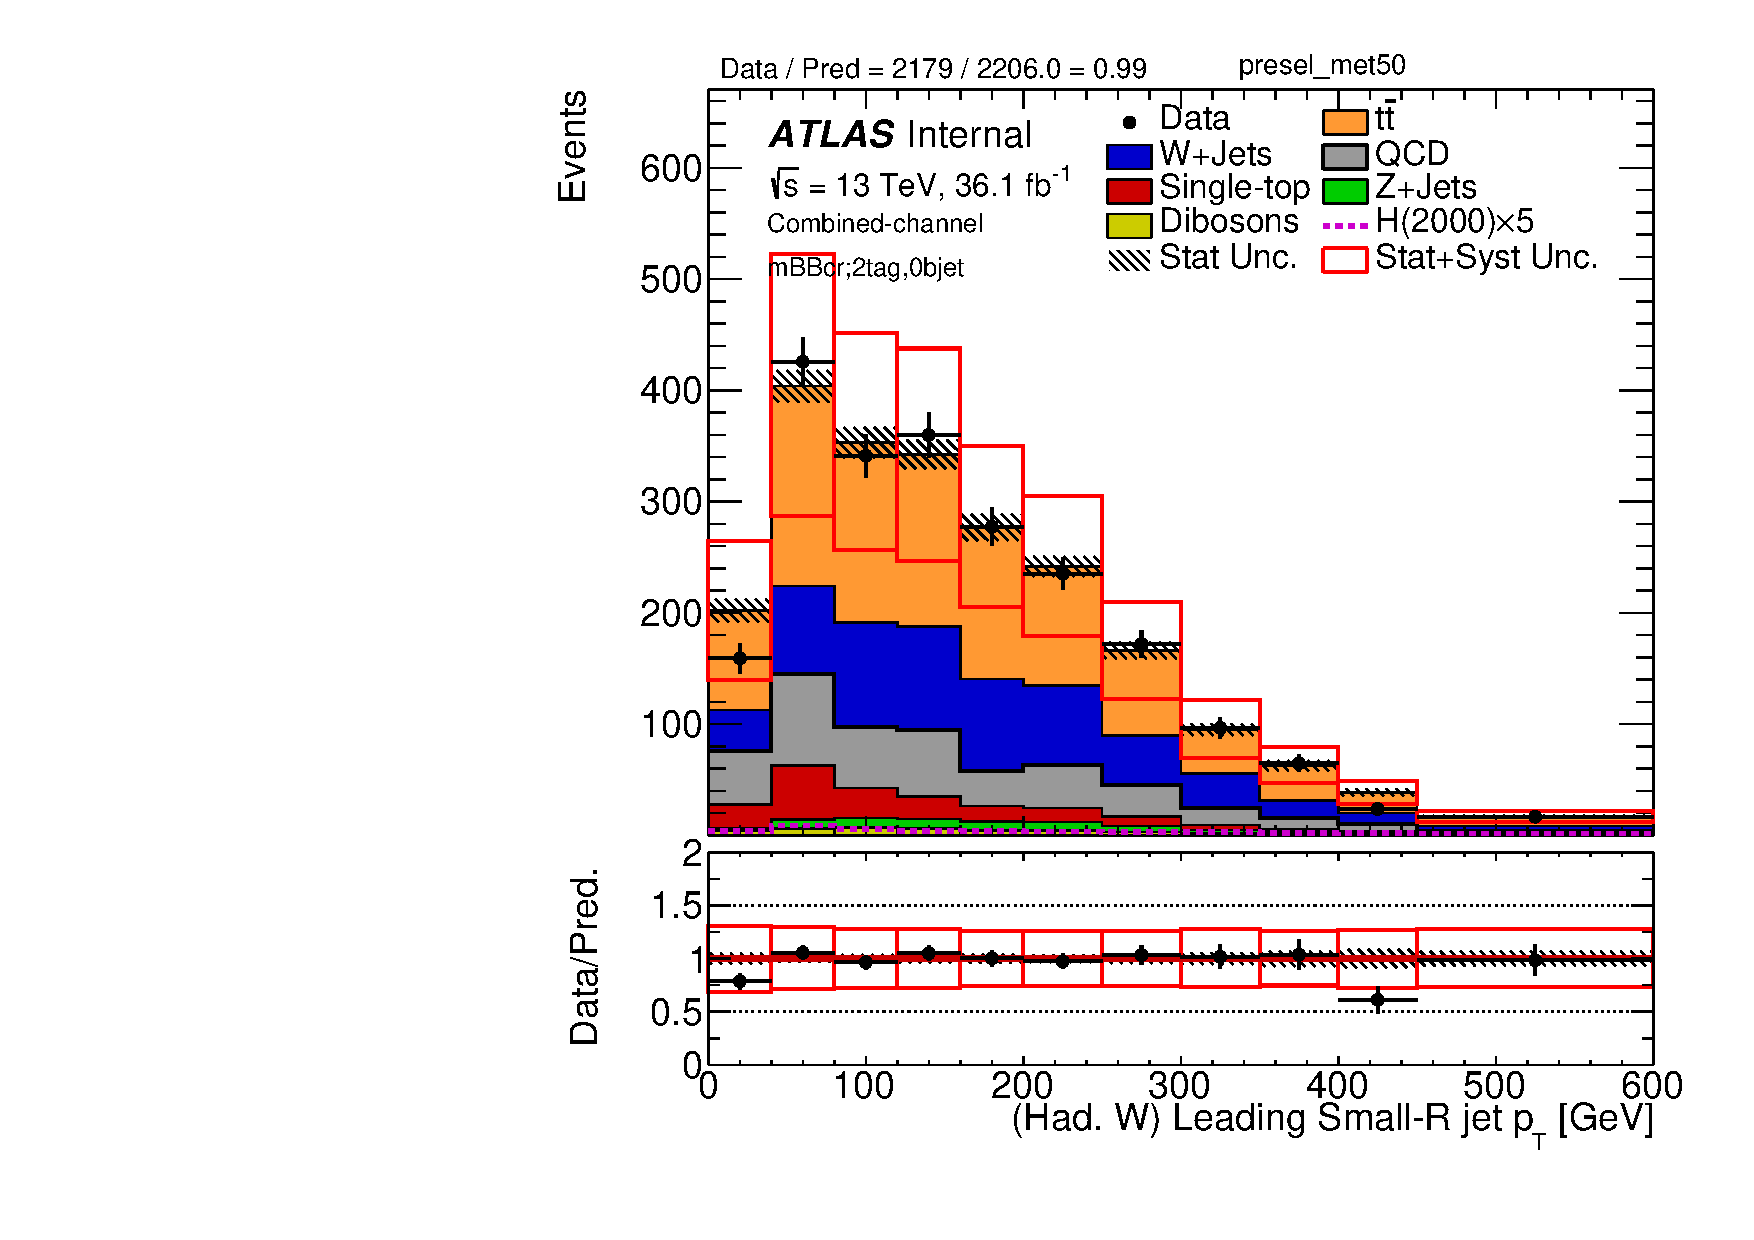
\includegraphics[scale=0.33]{./figures/boosted/PlotsInMbbCR/DataMC_2tag_0bjet_mbbcr_lepton_presel_met50_LightJet1Pt}
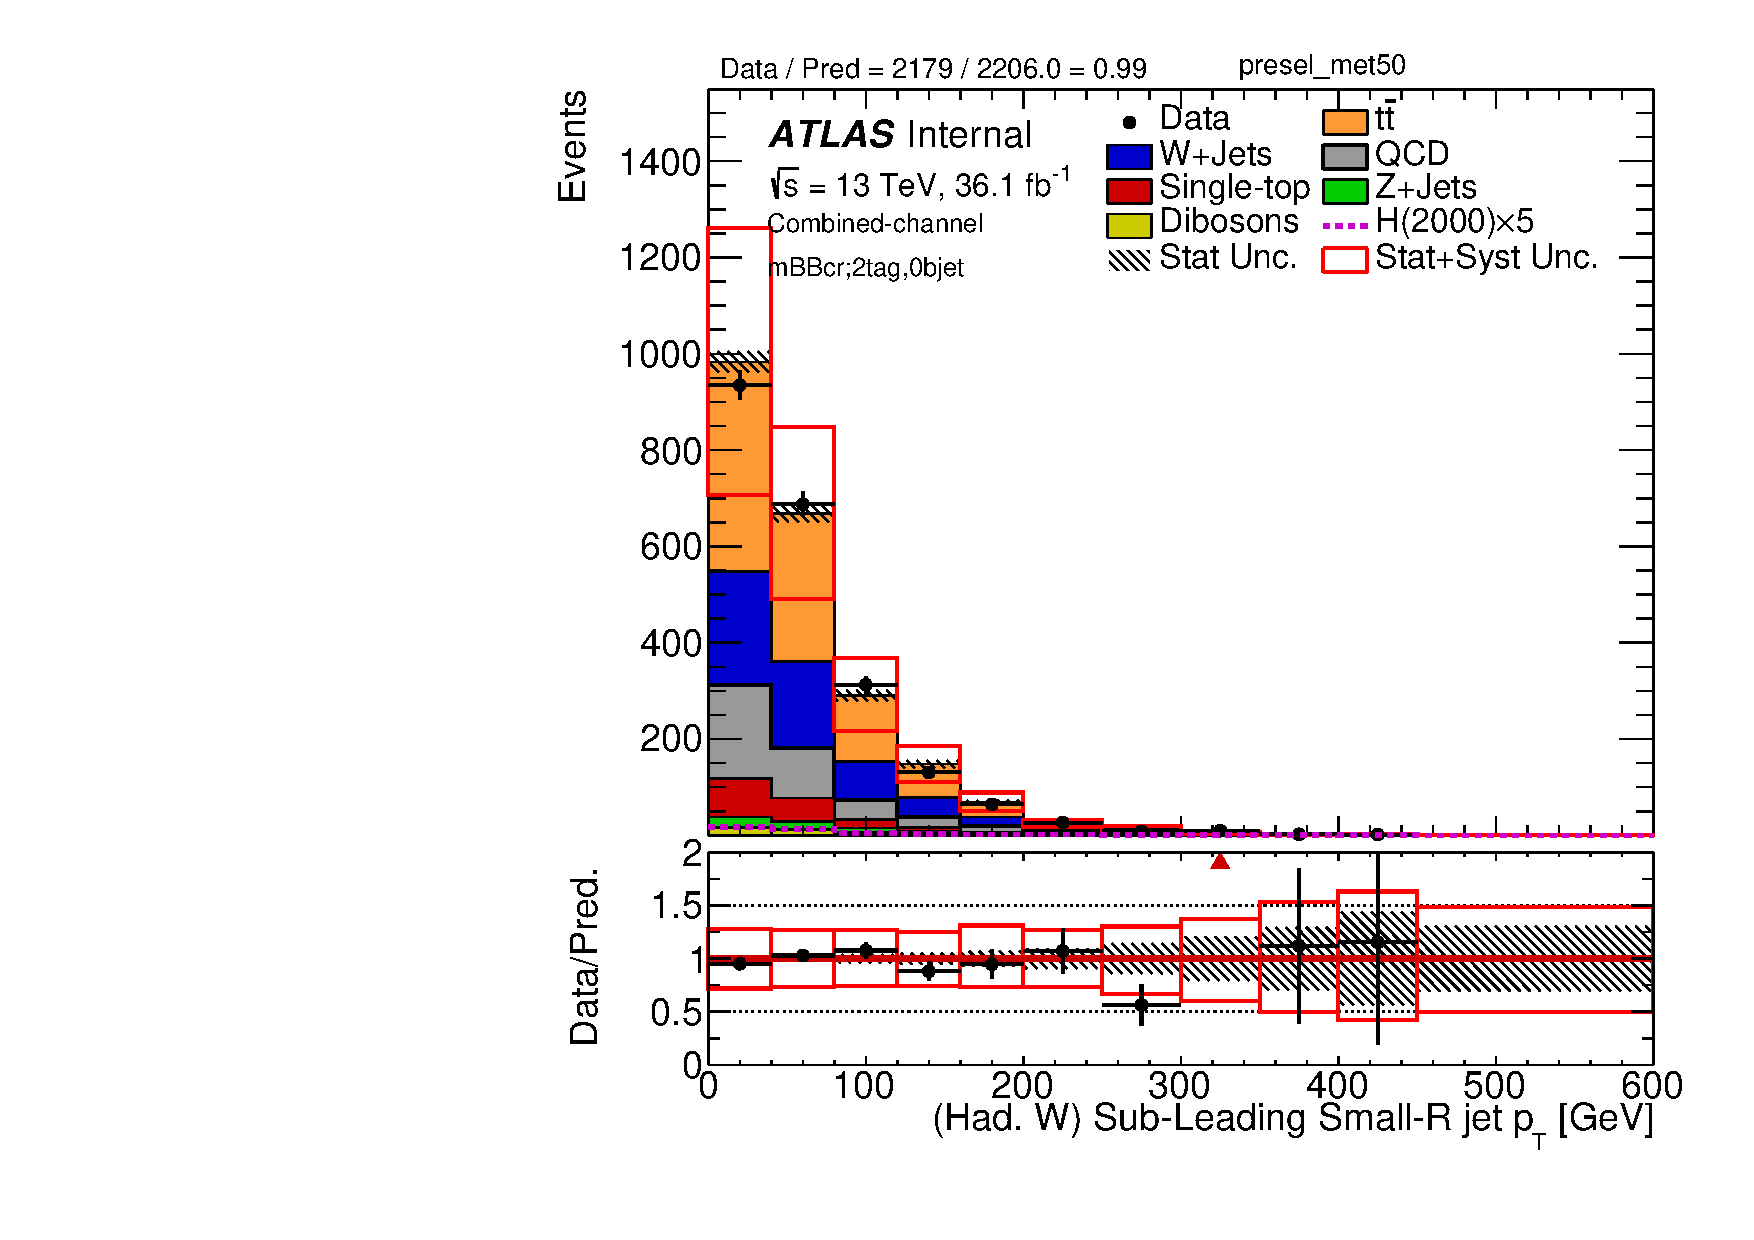
\includegraphics[scale=0.33]{./figures/boosted/PlotsInMbbCR/DataMC_2tag_0bjet_mbbcr_lepton_presel_met50_LightJet2Pt}\\
\par\medskip
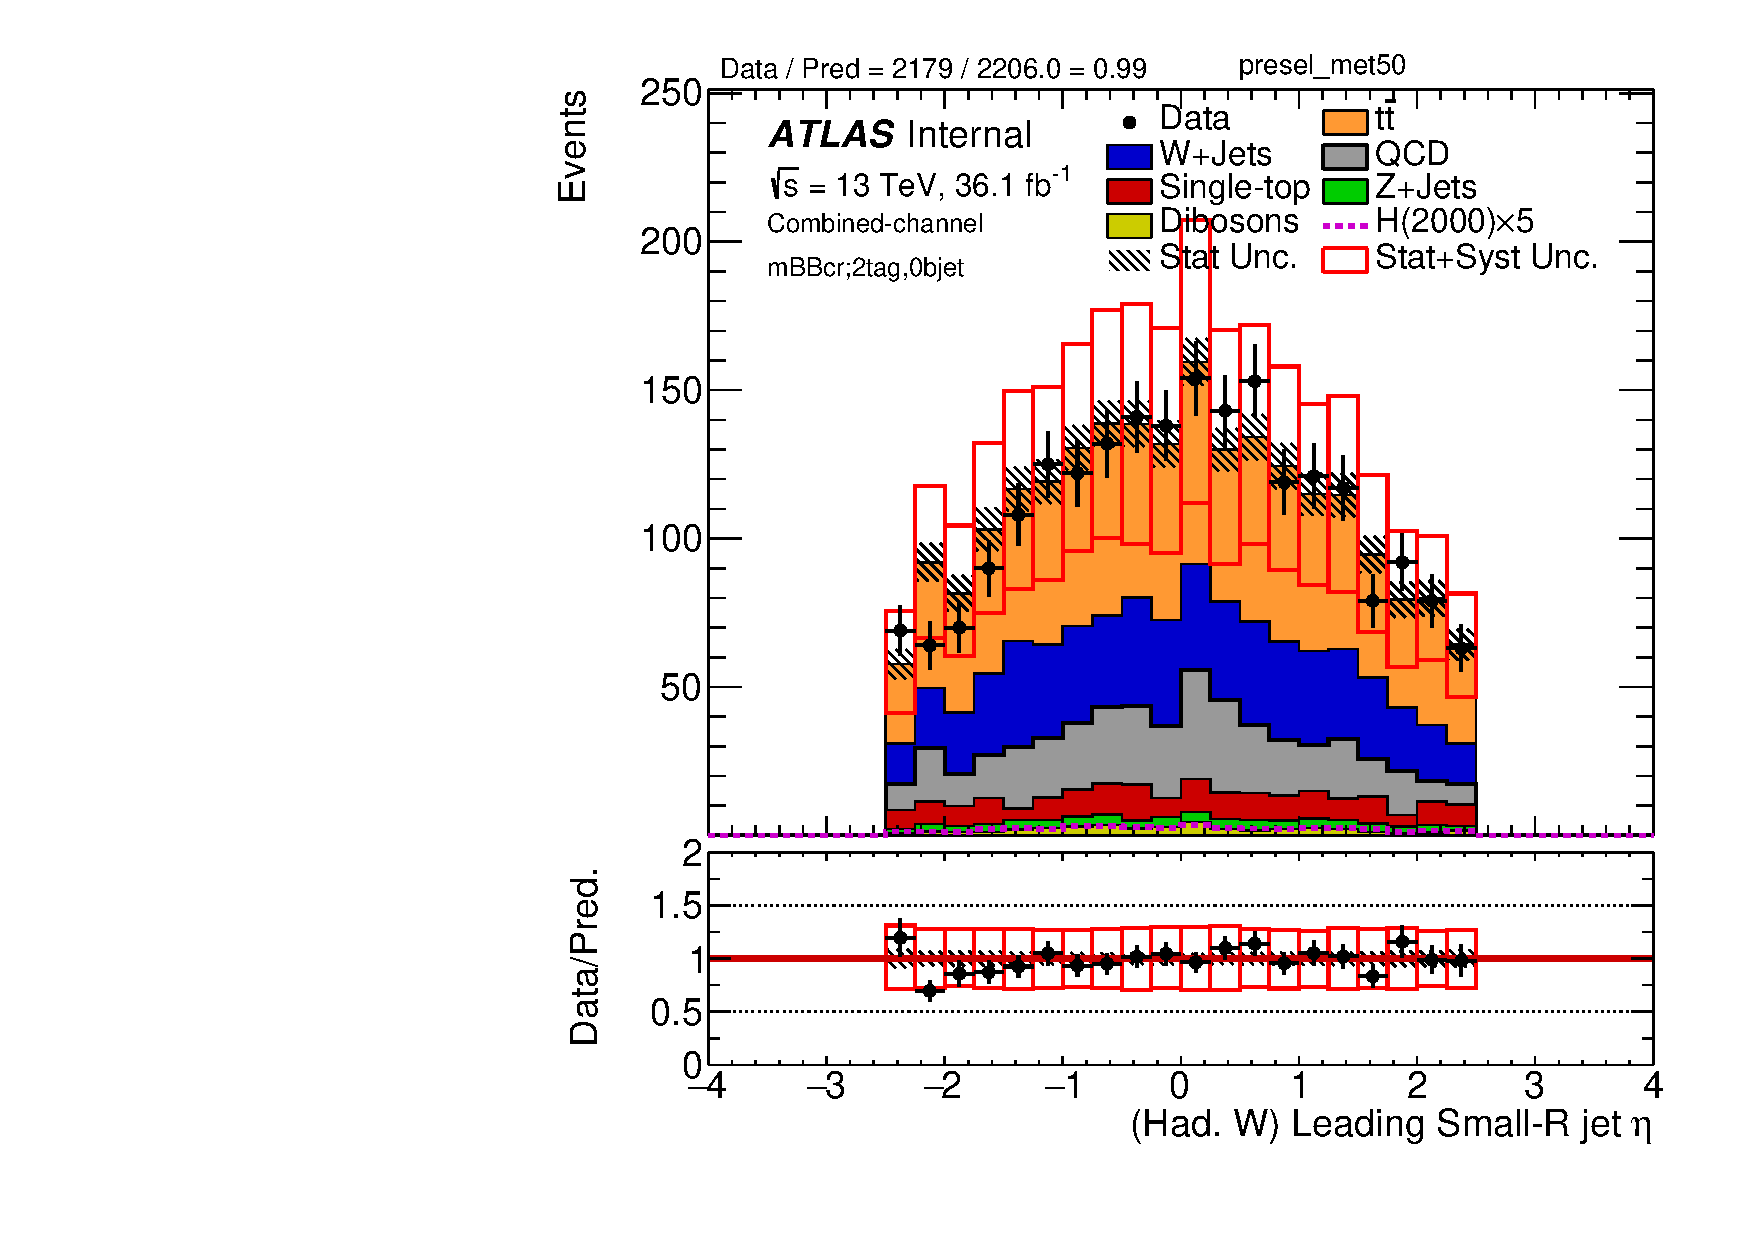
\includegraphics[scale=0.33]{./figures/boosted/PlotsInMbbCR/DataMC_2tag_0bjet_mbbcr_lepton_presel_met50_LightJet1Eta}
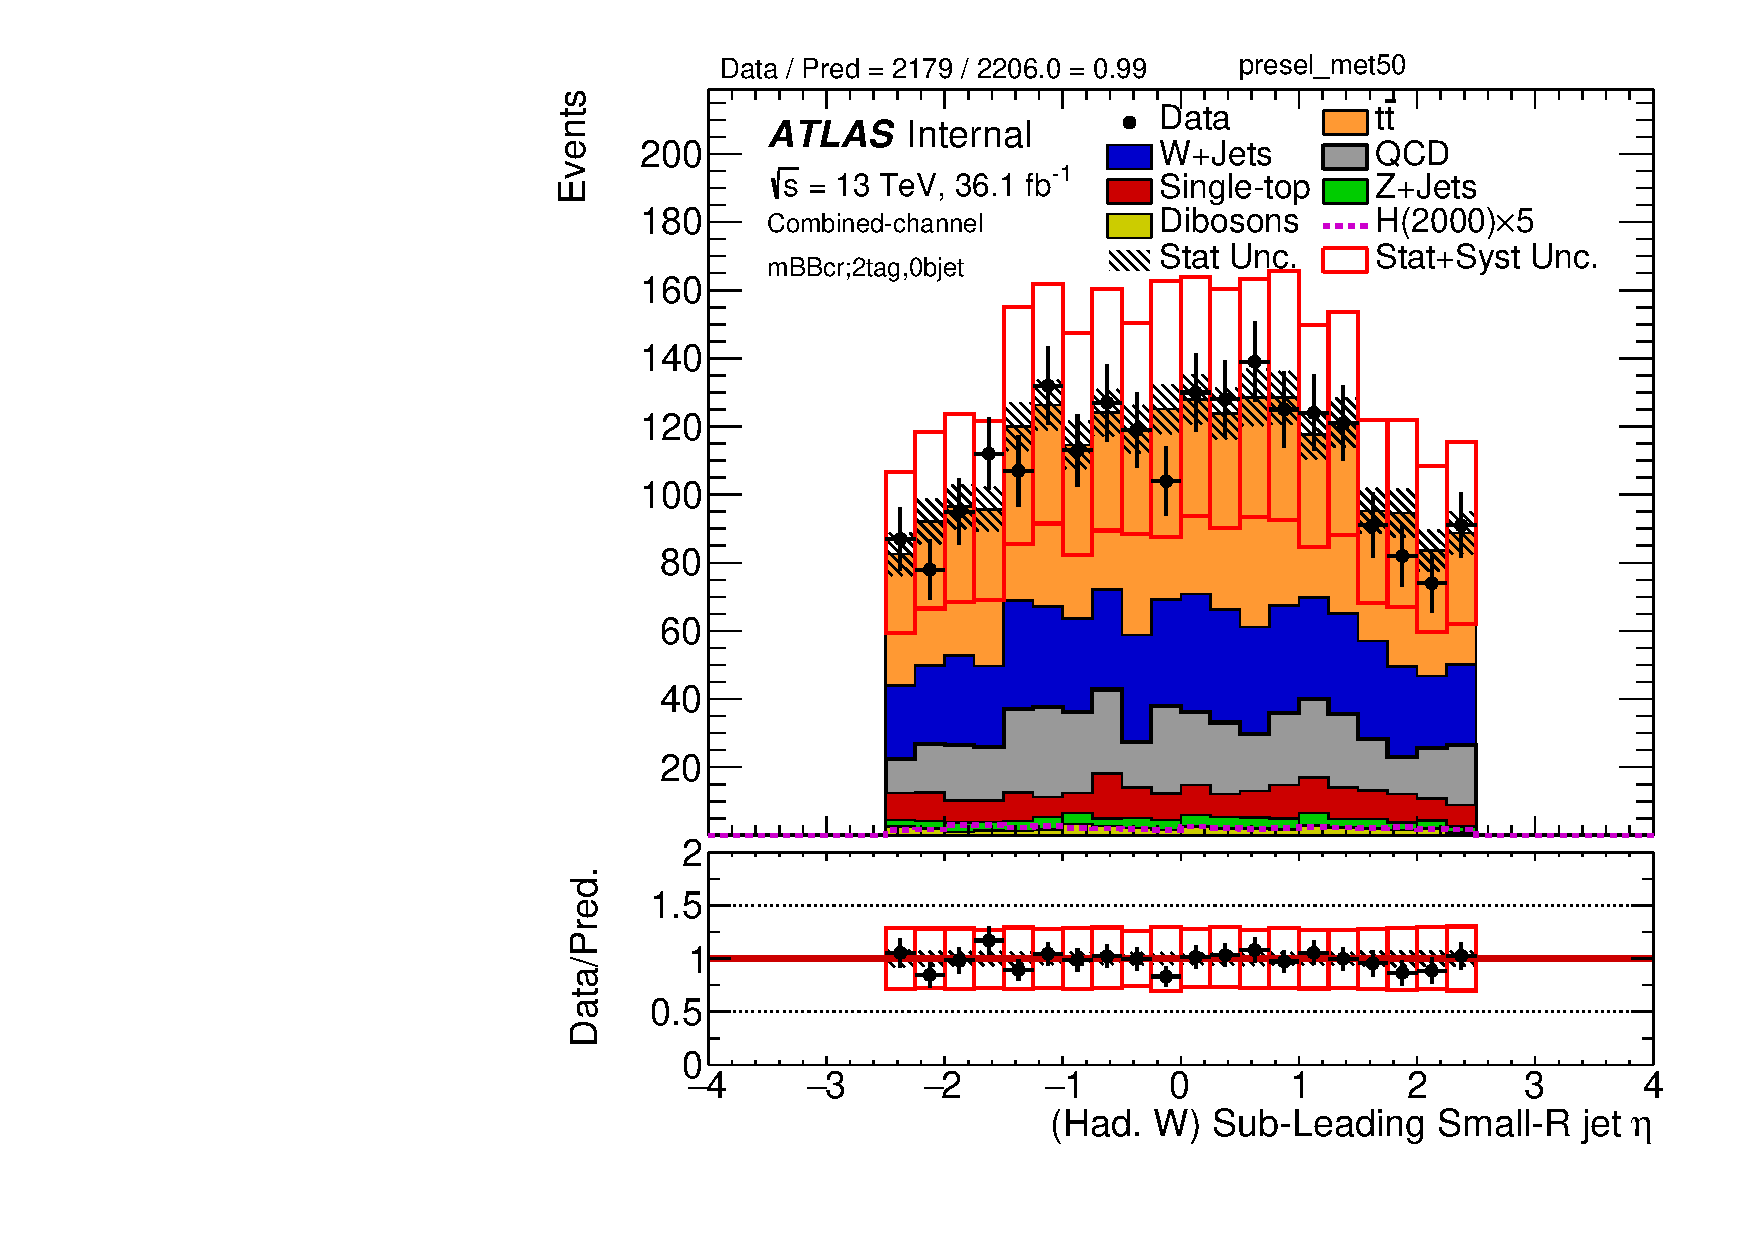
\includegraphics[scale=0.33]{./figures/boosted/PlotsInMbbCR/DataMC_2tag_0bjet_mbbcr_lepton_presel_met50_LightJet2Eta}\\
\par\medskip
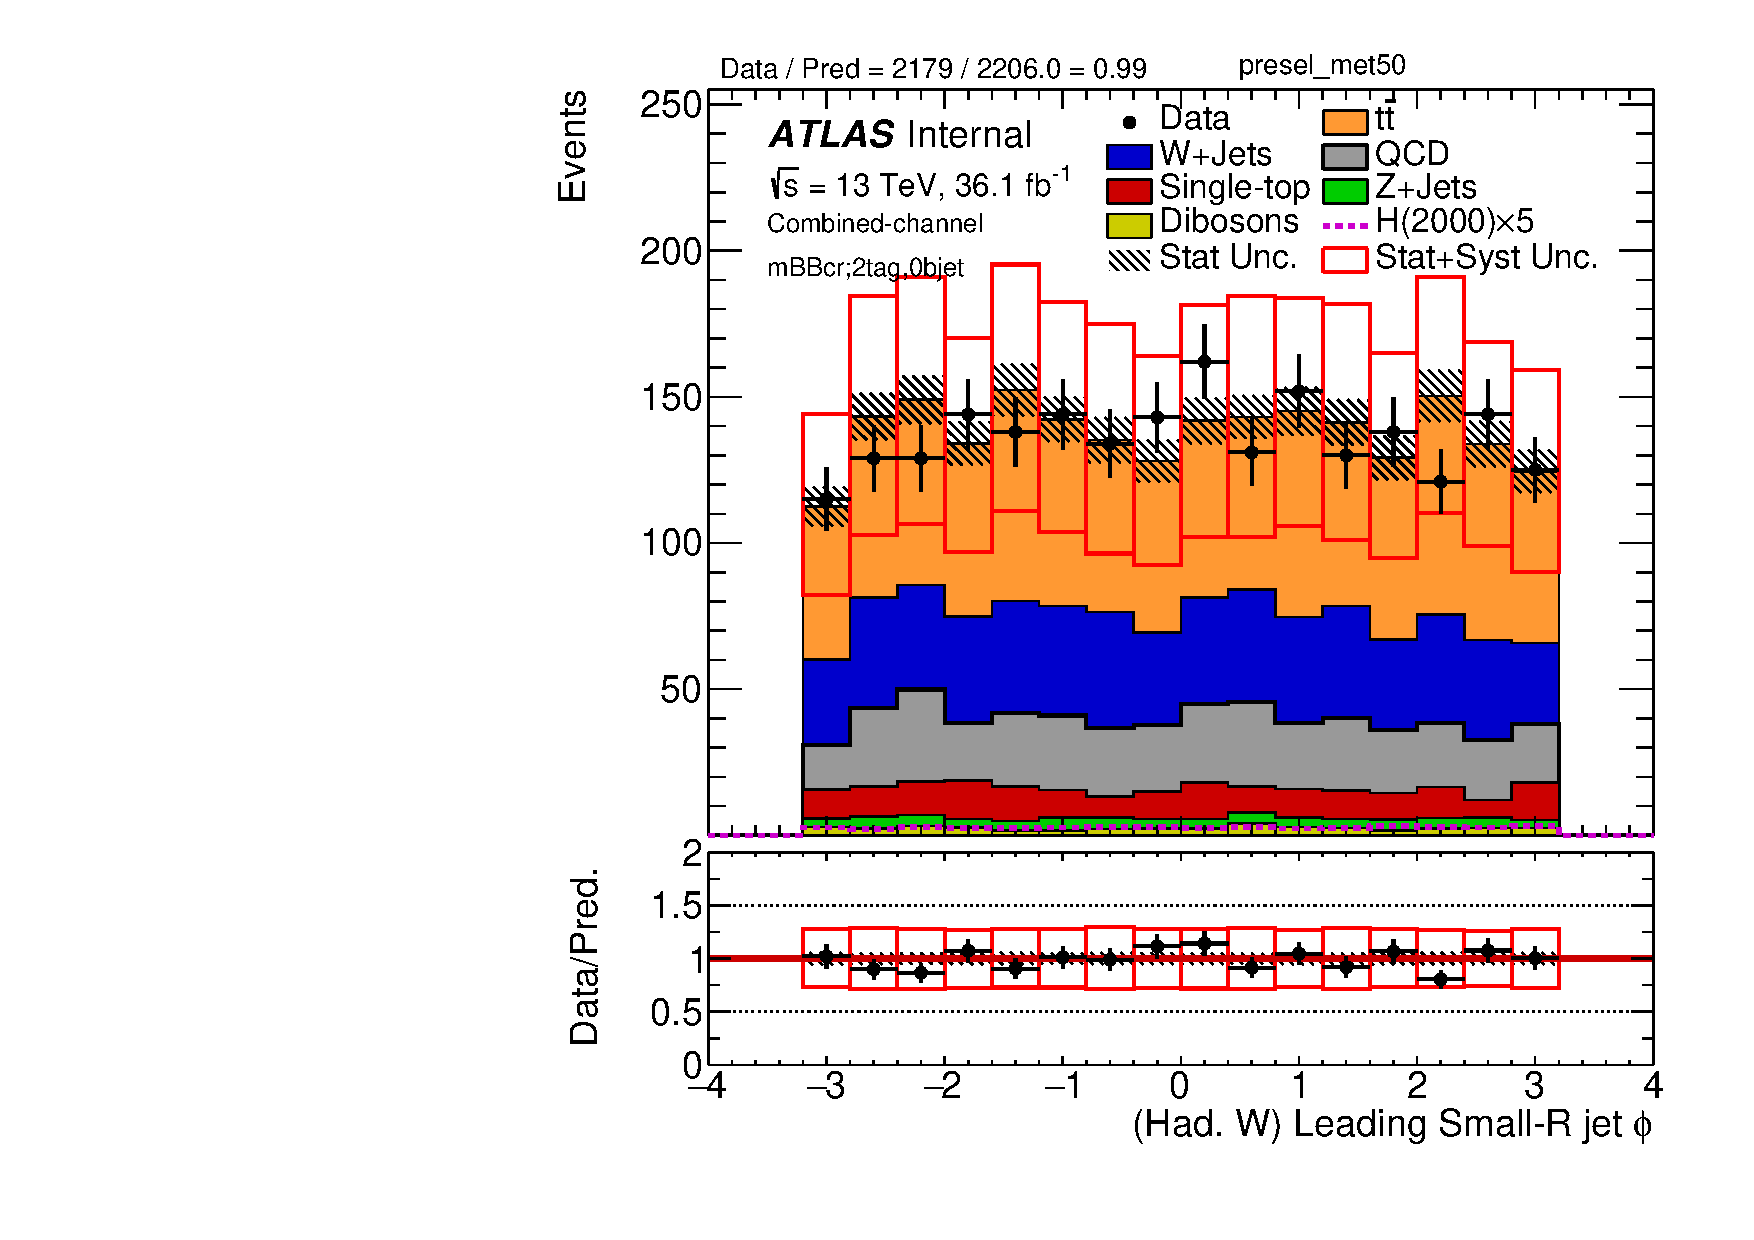
\includegraphics[scale=0.33]{./figures/boosted/PlotsInMbbCR/DataMC_2tag_0bjet_mbbcr_lepton_presel_met50_LightJet1Phi}
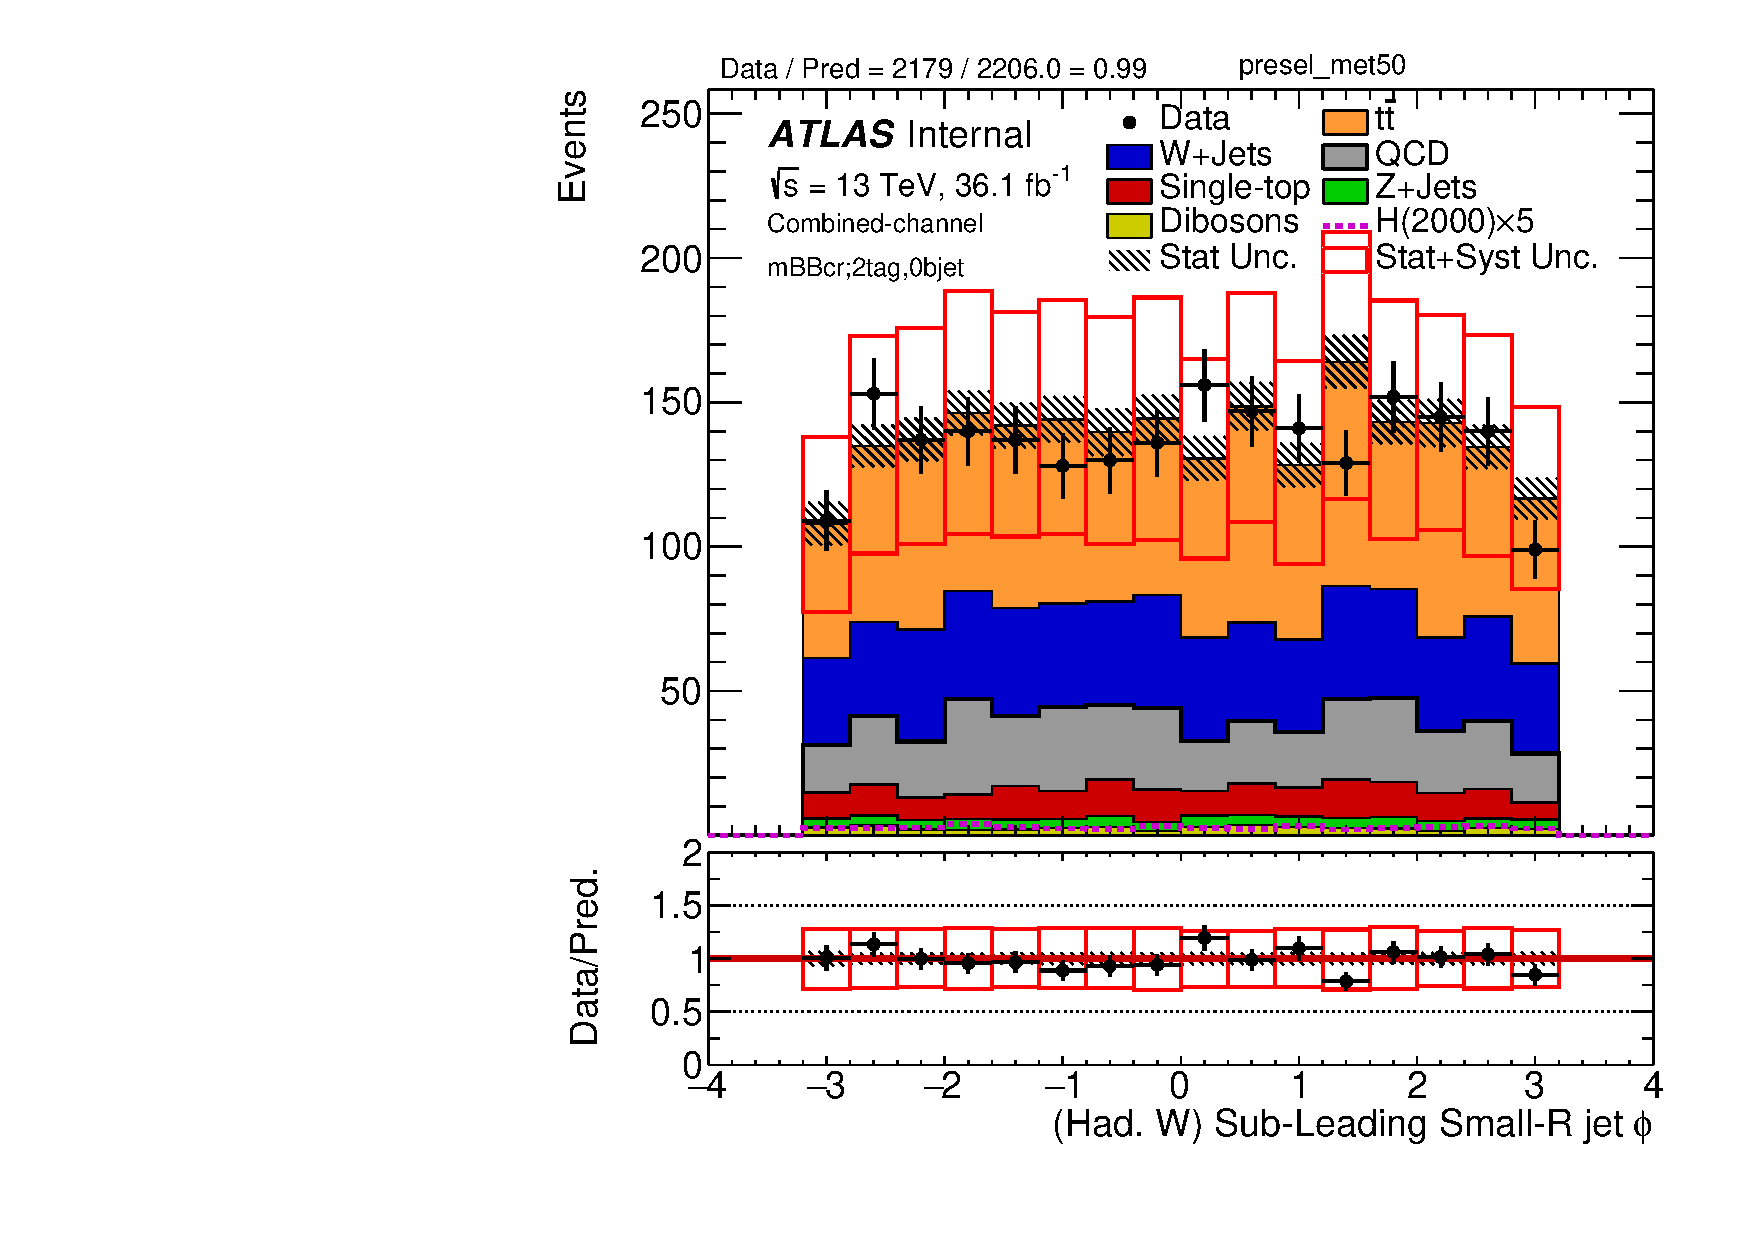
\includegraphics[scale=0.33]{./figures/boosted/PlotsInMbbCR/DataMC_2tag_0bjet_mbbcr_lepton_presel_met50_LightJet2Phi}\\
\caption{Kinematic distributions of the leading and sub-leading small-$R$ jets (of the reconstructed hadronic W)
in the mBB control region (mBBcr).}
\label{fig:boosted_mbbcr_whad_jets}
\end{center}
\end{figure}
 
\begin{figure}[!h]
\begin{center}
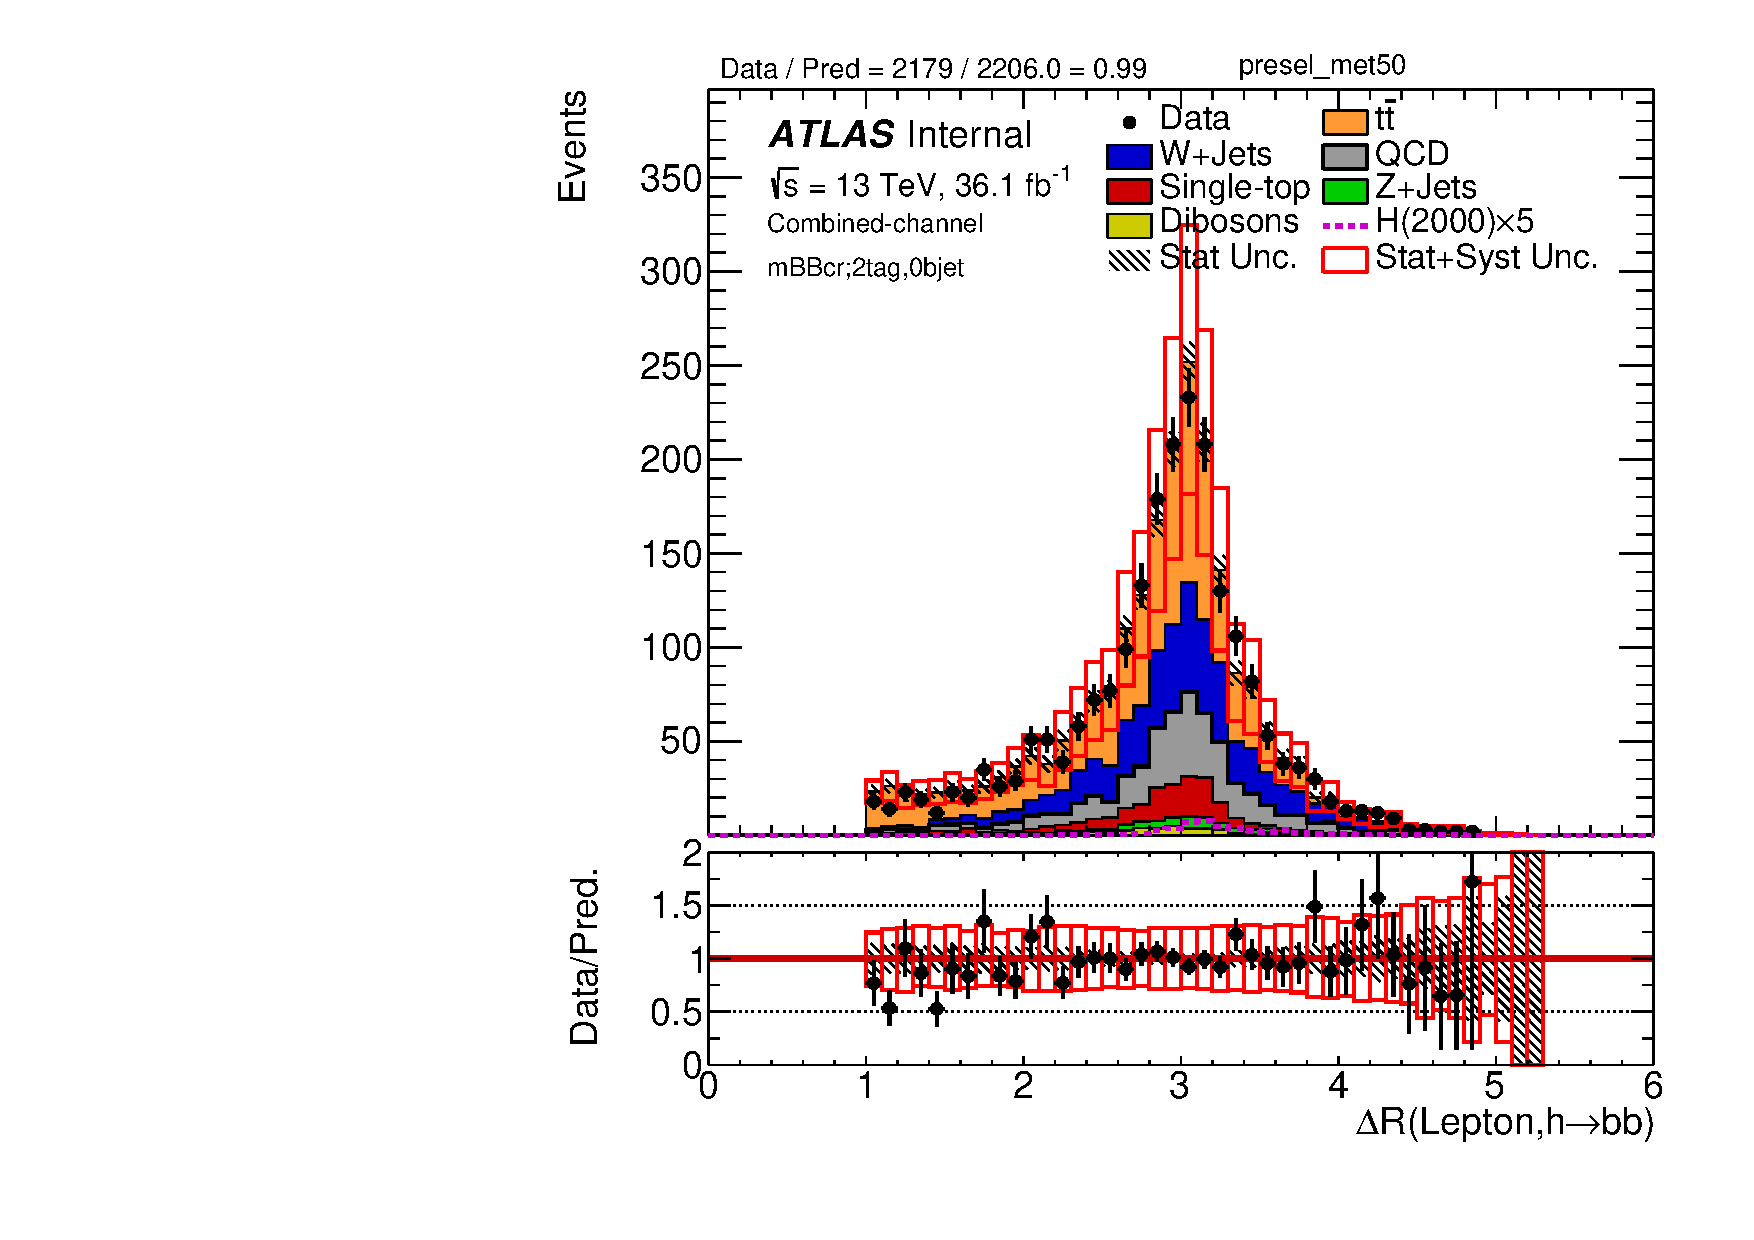
\includegraphics[scale=0.33]{./figures/boosted/PlotsInMbbCR/DataMC_2tag_0bjet_mbbcr_lepton_presel_met50_drHbbLep}
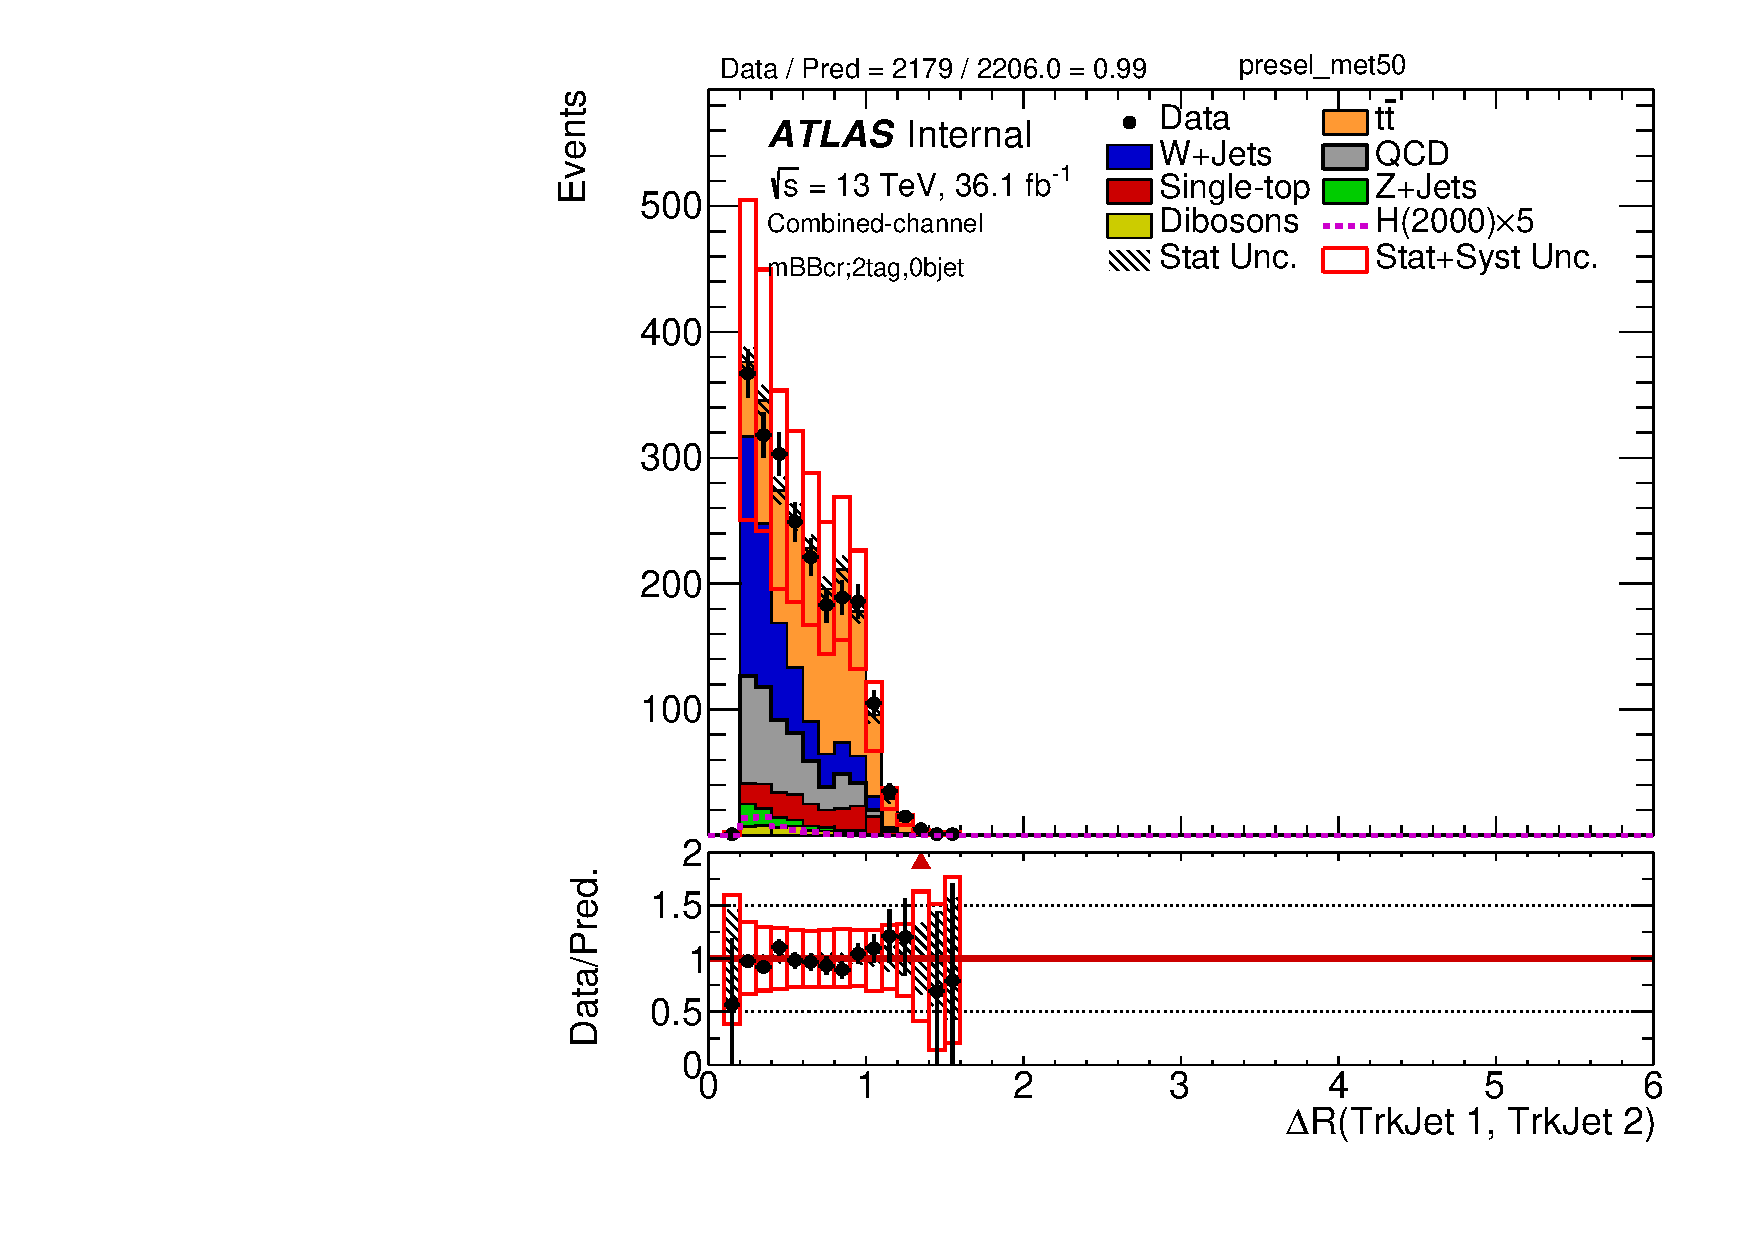
\includegraphics[scale=0.33]{./figures/boosted/PlotsInMbbCR/DataMC_2tag_0bjet_mbbcr_lepton_presel_met50_drbtrkjet1btrkjet2}\\
\caption{$\Delta R$ distribution between the selected lepton and the large-$R$ jet and $\Delta R$ distribution between the track-jets inside
the large-$R$ jet in the mBB control region (mBBcr).}
\label{fig:boosted_mbbcr_dr}
\end{center}
\end{figure}
 
\newpage
  
\subsection{Systematics}
\subsubsection{Dectector modeling uncertainties}
\label{sec:boosted_syst_detector}
 
The experimental uncertainties considered in the analysis are listed in Table~\ref{tab:boosted_syst_detector}.
The uncertainties are applicable to signal and background processes that are modelled using MC simulation.
 
\begin{table}
\resizebox{\textwidth}{!}
{
\begin{tabular}{l|l}
 
\hline
Systematic uncertainty & Short description \\
\hline
\multicolumn{2}{c}{Event} \\
\hline
\texttt{ATLAS\_LUMI\_2015\_2016} & uncertainty on total integrated luminosity \\
\hline
\texttt{PRW\_DATASF} & pile-up reweighting uncertainty \\
\hline
\multicolumn{2}{c}{Electrons} \\
\hline
\texttt{EL\_EFF\_Trigger\_TOTAL\_1NPCOR\_PLUS\_UNCOR} &  trigger efficiency uncertainty \\
\texttt{EL\_EFF\_Reco\_TOTAL\_1NPCOR\_PLUS\_UNCOR}         &  reconstruction efficiency uncertainty \\
\texttt{EL\_EFF\_ID\_TOTAL\_1NPCOR\_PLUS\_UNCOR}         &  ID efficiency uncertainty \\
\texttt{EL\_EFF\_Iso\_TOTAL\_1NPCOR\_PLUS\_UNCOR}          &  isolation efficiency uncertainty \\
\texttt{EG\_SCALE\_ALL} &        energy scale uncertainty          \\        
\texttt{EG\_RESOLUTION\_ALL} &    energy resolution uncertainty    \\  
\hline
\multicolumn{2}{c}{Muons} \\
\hline
\texttt{MUON\_EFF\_TrigStatUncertainty} &  \multirow{2}{*}{trigger efficiency uncertainty} \\  
\texttt{MUON\_EFF\_TrigSystUncertainty} &  \\
\texttt{MUON\_EFF\_STAT} &  \multirow{2}{*}{reconstruction and ID efficiency uncertainty for muons}\\  
\texttt{MUON\_EFF\_SYS} &  \\
\texttt{MUON\_ISO\_STAT} &  \multirow{2}{*}{isolation efficiency uncertainty}\\  
\texttt{MUON\_ISO\_SYS} & \\            
\texttt{MUONS\_SCALE} &    energy scale uncertainty        \\                  
\texttt{MUONS\_ID} & energy resolution uncertainty from inner detector     \\                  
\texttt{MUONS\_MS} &  energy resolution uncertainty from muon system  \\
\hline
\multicolumn{2}{c}{Small-$R$ jets} \\
\hline
\texttt{JET\_SR1\_JET\_GroupedNP\_1} & \multirow{4}{*}{energy scale uncertainties strongly-reduced to 4 components.} \\
\texttt{JET\_SR1\_JET\_GroupedNP\_2} & \\
\texttt{JET\_SR1\_JET\_GroupedNP\_3} & \\
\texttt{JET\_SR1\_JET\_EtaIntercalibration\_NonClosure} &  \\
\texttt{JET\_JER\_SINGLE\_NP} & energy resolution uncertainty  \\
\texttt{JET\_JvtEfficiency} & JVT efficiency uncertainty   \\
% \texttt{FT\_EFF\_Eigen\_B} & \multirow{3}{*}{\parbox{11cm}{$b$-tagging efficiency uncertainties (``BTAG\_MEDIUM''): 3 components for $b$ jets, 4 for $c$ jets and 5 for light jets}} \\
% \texttt{FT\_EFF\_Eigen\_C} & \\
% \texttt{FT\_EFF\_Eigen\_L} & \\
% \texttt{FT\_EFF\_Eigen\_extrapolation} & $b$-tagging efficiency uncertainty on the extrapolation to high-\pt jets  \\
% \texttt{FT\_EFF\_Eigen\_extrapolation\_from\_charm} & $b$-tagging efficiency uncertainty on tau jets   \\
\hline
\multicolumn{2}{c}{Large-$R$ jets} \\
\hline
\texttt{FATJET\_Medium\_JET\_Comb\_Baseline\_Kin}  &  \multirow{4}{*}{energy scale uncertainties (\pT and mass scales are fully correlated)} \\
\texttt{FATJET\_Medium\_JET\_Comb\_modeling\_Kin} &   \\
\texttt{FATJET\_Medium\_JET\_Comb\_TotalStat\_Kin} &   \\
\texttt{FATJET\_Medium\_JET\_Comb\_Tracking\_Kin}  &  \\
\texttt{FATJET\_JER} &  energy resolution uncertainty    \\
\texttt{FATJET\_JMR} &  mass resolution uncertainty \\
\hline
\multicolumn{2}{c}{Track-jets and Small-R jets} \\
\hline    
\texttt{FT\_EFF\_Eigen\_B} & \multirow{3}{*}{\parbox{11cm}{$b$-tagging efficiency uncertainties (``BTAG\_MEDIUM''): 3 components for $b$ jets, 4 for $c$ jets and 5 for light jets}} \\
\texttt{FT\_EFF\_Eigen\_C} & \\
\texttt{FT\_EFF\_Eigen\_L} & \\
\texttt{FT\_EFF\_Eigen\_extrapolation} & $b$-tagging efficiency uncertainty on the extrapolation to high \pt jets  \\
\texttt{FT\_EFF\_Eigen\_extrapolation\_from\_charm} & $b$-tagging efficiency uncertainty on tau jets  \\
\hline
\multicolumn{2}{c}{\met} \\
\hline    
\texttt{MET\_SoftTrk\_ResoPara} & track-based soft term related longitudinal resolution uncertainty   \\
\texttt{MET\_SoftTrk\_ResoPerp} & track-based soft term related transverse resolution uncertainty   \\
\texttt{MET\_SoftTrk\_Scale}    & track-based soft term related longitudinal scale uncertainty   \\  
\hline
\end{tabular}
}
\caption{Summary of the (nuisance parameter) names and meanings of the detector modeling systematic uncertainties.}
\label{tab:boosted_syst_detector}
\end{table}
 
\paragraph{$|d_{0}^{\textrm{sig}}|$ cut efficiency modeling}
\label{sec:boosted_syst_d0cut}
 
In this analysis, the $|d_{0}^{\textrm{sig}}|$ cut value used for electrons and muons are not the recommended
value by CP groups. The recommended value for electrons is 5 while for muons it is 3. The modeling of the
$|d_{0}^{\textrm{sig}}|$ significance is assesed in a top-enriched control region. The event reconstruction and selection
criteria for the top-enriched control region are exactly the same as outlined in Section~\ref{sec:boosted_evtreco}
to~\ref{sec:boosted_regiondefs} with the exception that the $b$-tagging requirement on the event is different.
For this control region, each event is required to have either the leading or sub-leading track-jet to be $b$-tagged but not both track-jets to $b$-tagged.
The event is also required to have at least one $b$-tagged signal small-$R$ jets, which is in other words the $b$-jet veto is reversed. For the purposes
of studying the modeling the of the $|d_{0}^{\textrm{sig}}|$ distribution, no $|d_{0}^{\textrm{sig}}|$ requirement is applied on the reconstructed leptons.
 
\begin{figure}[!htbp]
\begin{center}
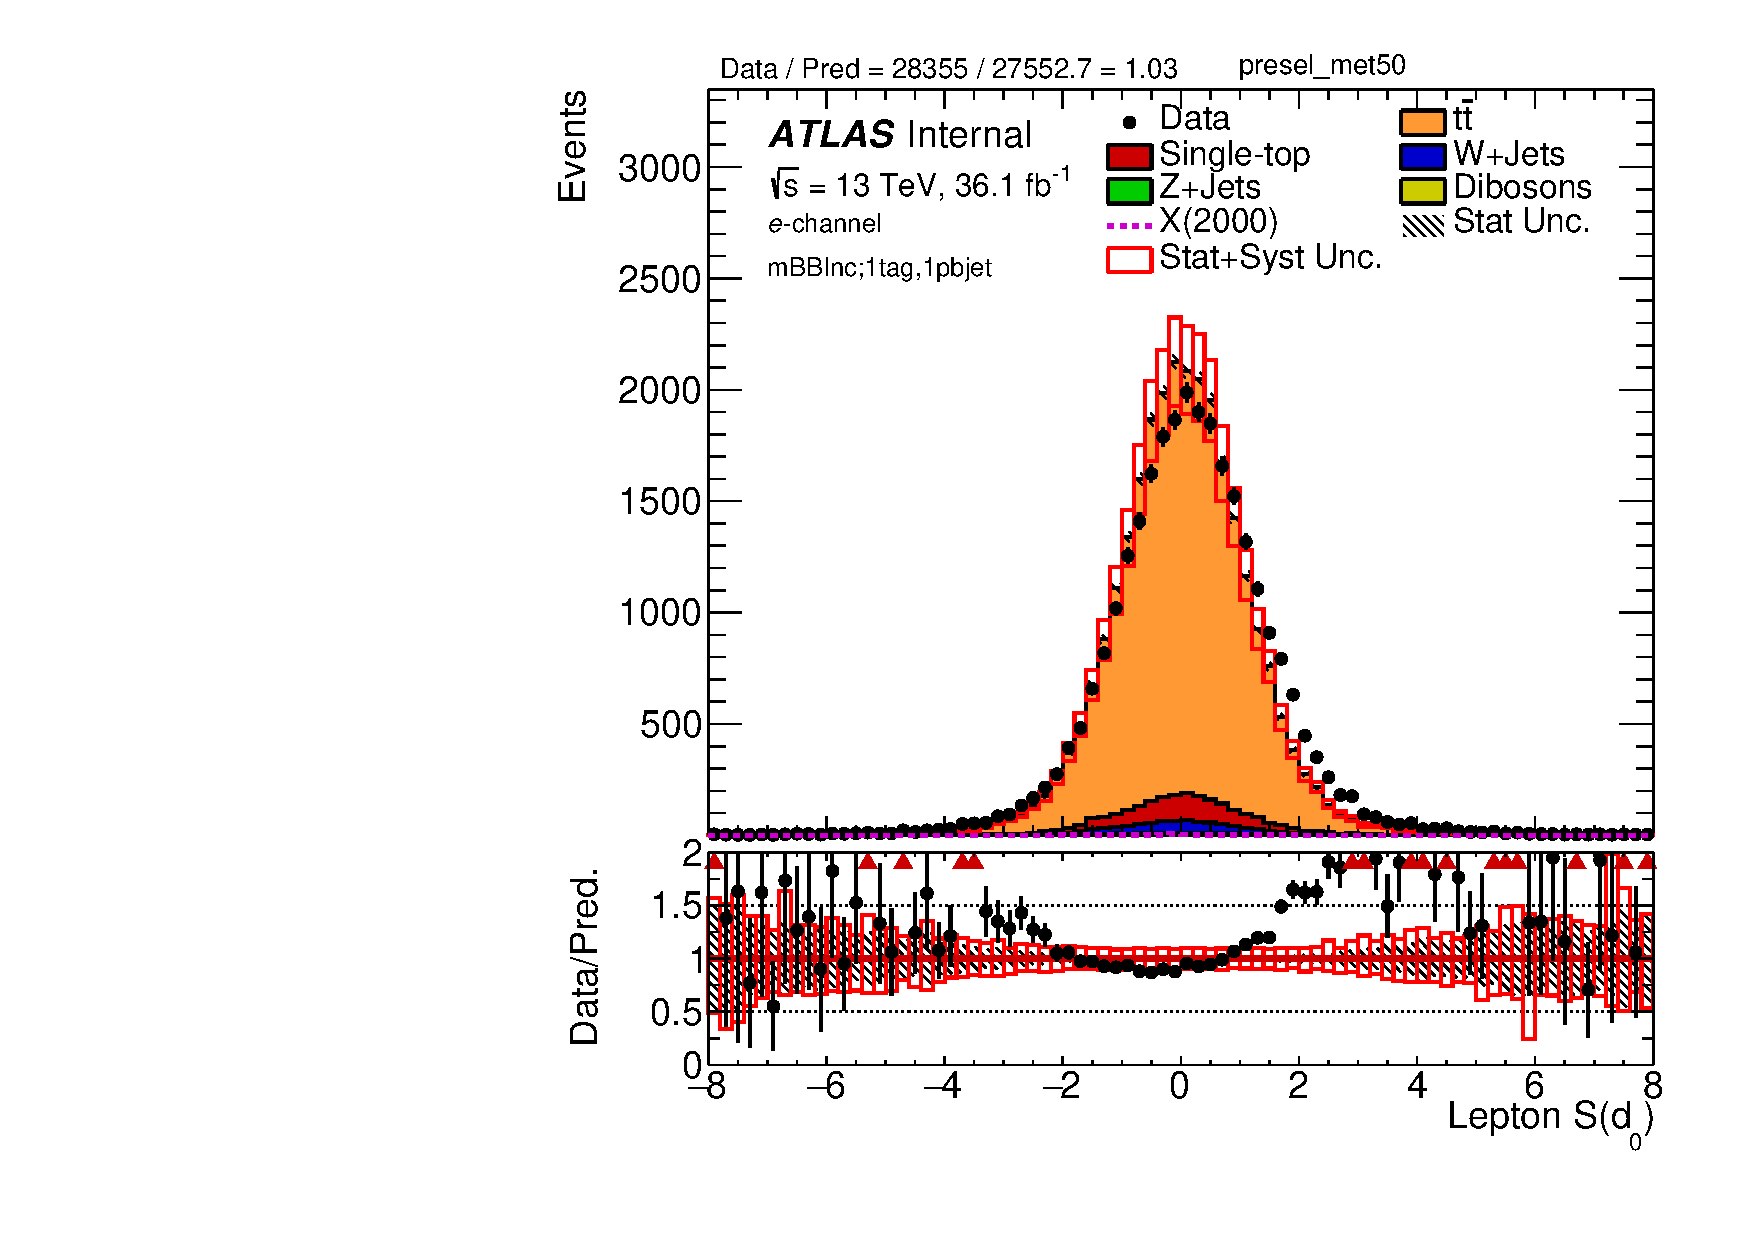
\includegraphics[scale=0.33]{./figures/boosted/Leptond0Plots/DataMC_1tag_1pbjet_Inc_elec_presel_met50_Lep_d0sigL} 
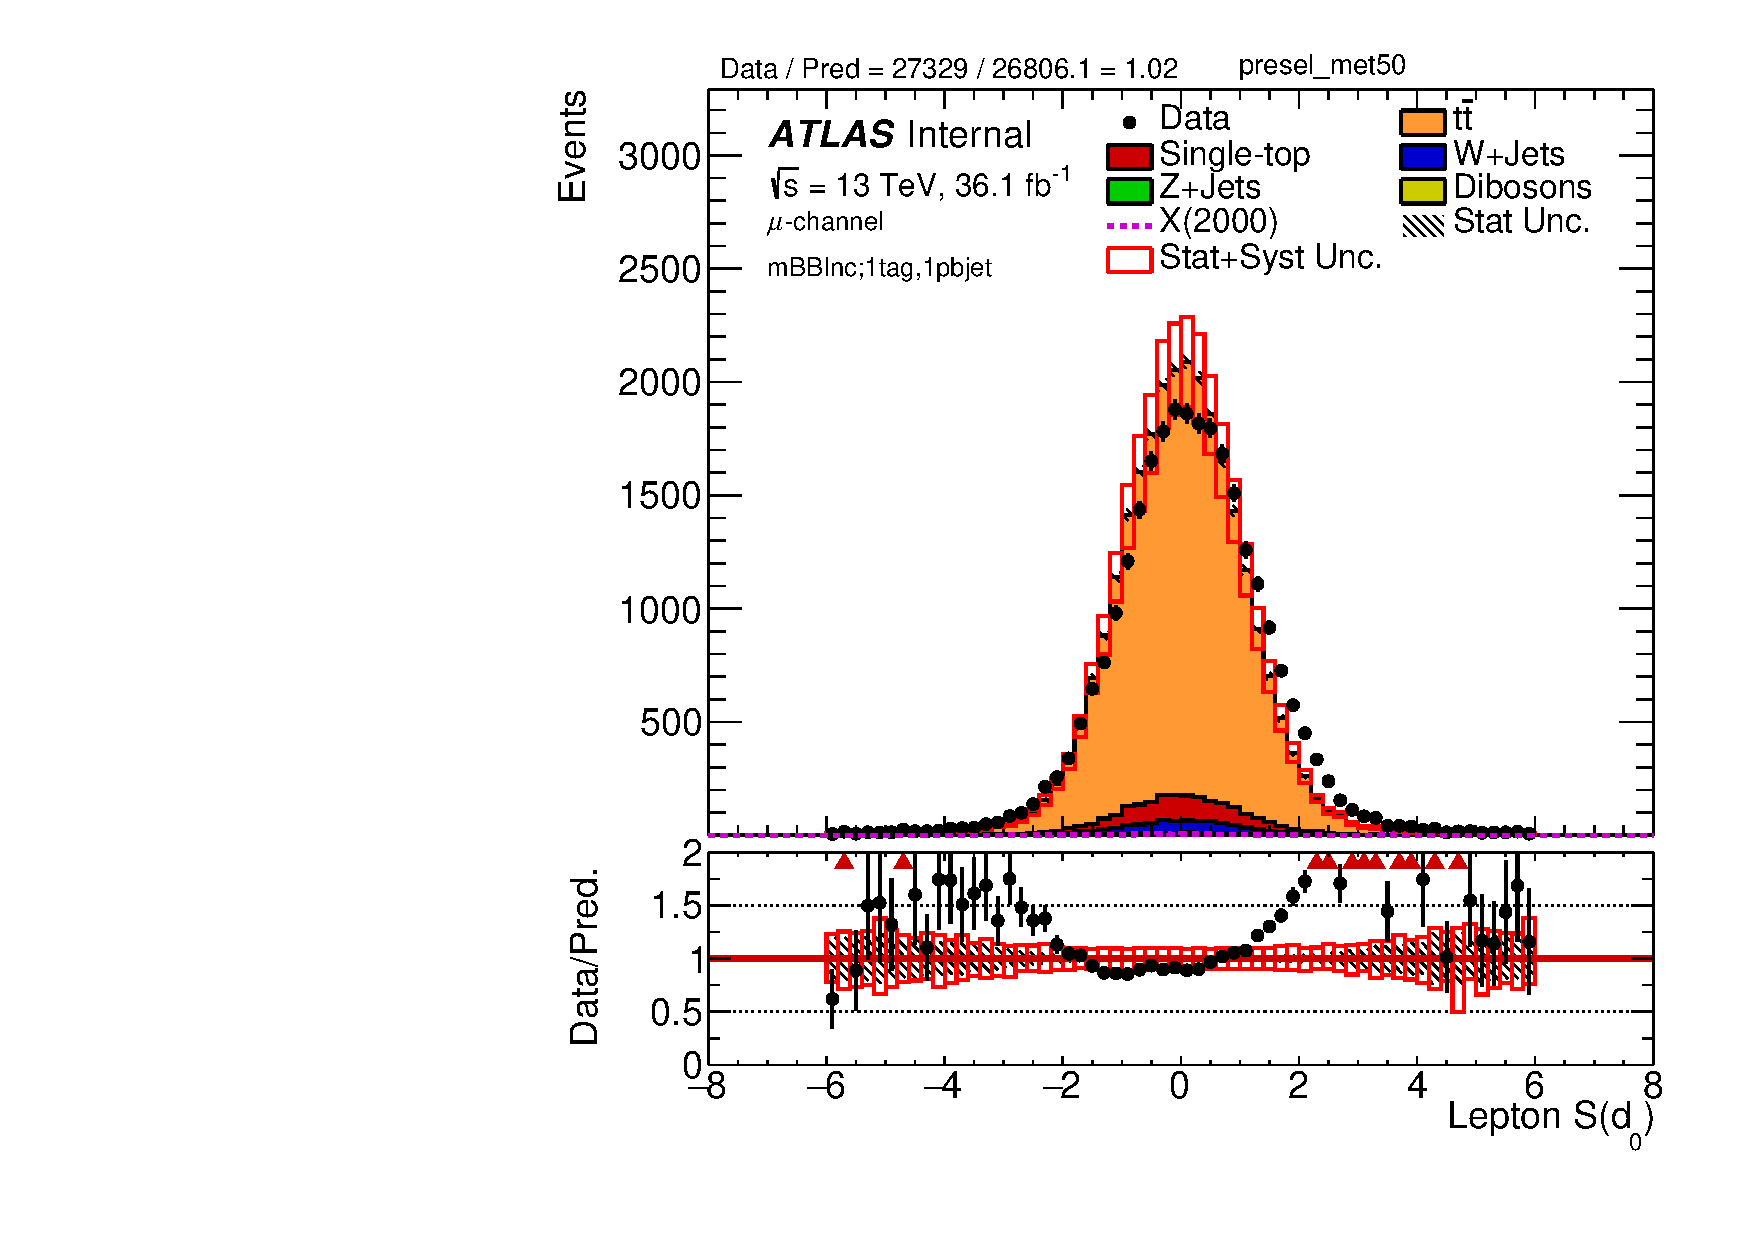
\includegraphics[scale=0.33]{./figures/boosted/Leptond0Plots/DataMC_1tag_1pbjet_Inc_muon_presel_met50_Lep_d0sigL} 
\caption{Electron and muon $d_{0}^{\textrm{sig}}$ distributions in the top control region without the large-$R$ jet mass cut.}
\label{fig:syst_d0_topcr}
\end{center}
\end{figure}
 
Figure~\ref{fig:syst_d0_topcr} shows the $|d_{0}^{\textrm{sig}}|$ distribution for the electron and the muon in the top-enriched control region. A clear bias
in Data can be observed and this is consistent with other studies throught ATLAS. In order to take into account the effect of the mismodeling of the $d_{0}^{\textrm{sig}}$
bias on the tight $d_{0}^{\textrm{sig}}$ cut used in this analysis, the efficiency of the $|d_{0}^{\textrm{sig}}|$ cut is evaluated and compared between Data and MC.
Table~\ref{tab:syst_d0_topcr_eff_datamc} shows the efficiency of the $|d_{0}^{\textrm{sig}}|$ cut in Data and MC and the ratio of effieciency between Data and MC in each
lepton channel. The relative difference between Data/MC ratio and unity is taken as the uncertainty on the $|d_{0}^{\textrm{sig}}|$ significance cut efficiency
and it is assigned for all processes with prompt leptons modelled by MC simulation. The nuisance parameter name associated to this uncertainty is \texttt{LEP\_d0\_CutEff}
 
\begin{table}[!htbp]
\begin{center}
\begin{tabular}{c|c|c}
&  Electron  & Muon  \\  
\hline
\multicolumn{3}{c}{$|d_{0}^{\textrm{sig}}|$ < 2.0} \\
\hline
Data                &  0.884  & 0.897 \\
MC                  &  0.926  & 0.937 \\
\hline
Data/MC             &  0.955  & 0.957 \\
\hline
\hline
\multicolumn{3}{c}{$|d_{0}^{\textrm{sig}}|$ > 2.0} \\
\hline
Data                &  0.115  & 0.104  \\
MC                  &  0.074  & 0.063  \\
\hline
Data/MC             &  1.572  & 1.640  \\
\end{tabular}
\end{center}
\caption{Efficiency of the $|d_{0}^{\textrm{sig}}|$ cut for electrons and muons in Data
and MC. The Data/MC ratio is also calculated and the difference between the ratio and unity
is taken as the systematic uncertainty on the $|d_{0}^{\textrm{sig}}|$ efficiency modeling
for events with leptons that pass (< 2.0) or fail (> 2.0) the $|d_{0}^{\textrm{sig}}|$ cut.}
\label{tab:syst_d0_topcr_eff_datamc}
\end{table}
 
\FloatBarrier
%---------------------------------------------------------------------------------------------------------------
 
\subsubsection{Background and Signal modeling Systematics}
\label{sec:boosted_syst_modeling}
 
%---------------------------------------------------------------------------------------------------------------
 
\paragraph{Methodology}
\label{sec:boosted_syst_modeling_method}
 
Uncertainties in the $m_{hh}$ distributions are assigned to the dominant backgrounds, $t\bar{t}$ and V+Jets and
single top by comparing the nominal MC samples to a number of alternative MC generators at the reconstruction
level. The comparisons are performed in with the same event selection in Sect~\ref{sec:Boosted}.
Each uncertainty contains 2 components, a shape systematic and a normalization systematic due to acceptance.
 
The shape systematic corresponds to a reweighting function derived by fitting a 1$^\text{st}$ order polynomial to the
ratio of $m_{hh}$ distribution of the variation sample over the nominal sample. The $m_{hh}$ distribution for the
the variation sample is normalized to the same number of events of the norminal sample.
 
% \begin{equation}
% \label{eq:MCShapeSystFormula}
% \frac{h^{var}_{i}}{h^{nom}_{i}}
% \end{equation}
 
% Where $h^{nom}_{i}$ ($h^{var}_{i}$) corresponds to the $i^{th}$ $m_{hh}$ bin of the nominal (variation) MC sample.
 
% Differences in the normalisation of each fit region can also be tested using the MC-to-MC comparisons, and are incorporated into the fit as
% a nuisance parameter $\theta_{k}$ that controls the relative ratio of two coupled regions. A single nuisance paramter controls the relative ratio
% of each set of coupled fit regions denoted as $R = \frac{A}{B}$, where $A/B$ represent a pair of coupled analysis fit regions that satisfy the
% condition $A \neq B$. The sets of coupled regions are as follows: $A/B = [\{SR,CR\}(\text{1-lep only}), \, \{0-lep,1-lep\}, \, \{1-lep,2-lep\},
% \, \{SR,topemucr\}(\text{2-lep only}), \, \{Resolved,Boosted\}]$. Each nuisance parameter is constrained using a prior uncertainty ($\sigma_{w_{accept}}$)
% derived from the MC-to-MC comparisons, where a $\theta(\frac{A}{B})_{k} = \pm 1$ pull corresponds to a $1 \pm 1\sigma_{w_{accept}}$ scale factor on the
% physical process in the numerator region ($A$ in this case). The prior uncertainty is derived using the formula:
 
% \begin{equation}\label{eq:MCAcceptanceSystFormula}
%  \sigma_{w_{accept}} = \sqrt{ \sum^{M}_{i}  \Bigg(\frac{ { \Big|\frac{n^{var^{i}}_{A}}{n^{var^{i}}_{B}}  - \frac{n^{nom}_{A}}{n^{nom}_{B}}\Big| } }{ \frac{n^{nom}_{A}}{n^{nom}_{B}} }\Bigg)^{2} }
% \end{equation}
 
% Where $n$ correponds to the total event yield, $M$ represents the total number of MC comparisons made for each physical process (see subsections \ref{sec:boosted_syst_modeling_top} \& \ref{sec:boosted_syst_modeling_vjets}), and the subscripts A/B denote the two coupled fit regions. The superscripts \textit{nom} \& $var^{i}$ denote the nominal MC and $i^{th}$ variation samples. When multiple MC-to-MC comparisons are made ($M \geq 2$), then quadrature sum of the individual priors is taken. As outlined in section \ref{sec:StatAnalysis}, each nuisance parameter is modelled as a log-normal (or Gaussian) distribution with an associated width parameter (width of the underlying Gaussian $\sigma$); this Gaussian constraint is defined by the above acceptance variation factor.
 
 
 
%---------------------------------------------------------------------------------------------------------------
 
\paragraph{Top-quark processes ($t \bar{t}$ \& single top) }
\label{sec:boosted_syst_modeling_top}
 
Four alternative MC $t \bar{t}$ samples are used to assess 3 aspects of the MC modeling,
whilst five alternative MC samples are used to assess 4 aspects of the MC modeling for
single top quark pair production. The alternative samples considered are:
 
\begin{itemize}
\item \textbf{\POWHEG+Herwig++:} The ME \POWHEG \;generator uses the same setup as that used for the nominal \POWHEG+\PYTHIA6 configuration,
but the parton shower (PS) generator is swapped out for Herwig++ version 2.7.1 using the UE-EE-5 tune and CTEQ6L1 PDF set.
The purpose therefore of this comparison is to test the PS, hadronisation, underlying event (UE) and Multiple Parton Interation (MPI) models
whilst maintaining the same hard scattering model given by \POWHEG.
 
\item \textbf{aMC@NLO+Herwig++:} The ME generator is swapped out for aMC@NLO using the CT10 PDF set, interfaced with Herwig++
using the CTEQ6L1-UE-EE-5 tune and CTEQ6LI PDF set. This sample is compared to the previous \POWHEG+Herwig++ sample.
This fixes the PS generator component, but alters the hard scattering generator, making this variation sensitive to the hard scatter model.
 
\item \textbf{\POWHEG+\PYTHIA6 Radhi/RadLo:} Using the same setup as that used for the nominal \POWHEG+\PYTHIA6 sample,
the RadHi and RadLo samples correspond to either the enhancement (high) or reduction (low) of initial/final state radiation (IFSR).
The two samples are compared to the nominal sample setup, and so are sensitive to variations of IFSR models.
   \begin{itemize}
   \item RadHi: The renormalisation ($\mu_{R}$) and factorisation scale ($\mu_{F}$) scales are decreased by a factor of 0.5,
   the \POWHEG \, \textsf{hdamp} parameter is doubled ($2 \times m_{top}$), and the high radiation PERUGIA2012 tune is used.
   \item RadLo: The renormalisation ($\mu_{R}$) and factorisation scale ($\mu_{F}$) scales are increased by a factor of 2,
   the \POWHEG \, \textsf{hdamp} parameter is kept at $m_{top}$, and the low radiation PERUGIA2012 tune is used.
   \end{itemize}
 
\item \textbf{\POWHEG+\PYTHIA6 Diagram Subtraction:} For the production of a single top quark in association with a W-boson ($Wt$)
the interference with the $t\bar{t}$ production process at NLO in QCD is removed by subtracting the cross-section
associated with the $t\bar{t}$ double resonance amplitude terms, rather than subtracting the same terms from the
amplitude prior to the calculation (Diagram Removal).
\end{itemize}
 
Table~\ref{tab:boosted_unc_ttbar} shows the estimated uncertainty on the normalization of the $t\bar{t}$ background in the signal region
from the comparison of the nominal $t\bar{t}$ sample to the alternative samples. The largest uncertainty comes the RadLo variation,
which is about \textasciitilde8.4\% with similar level of uncertainties from alternative ME generator choice and alternative PS generator choice.
The normalization of $t\bar{t}$ background is assinged with a single nuisance parameter with the total uncertainty set as the prior uncertainty.
 
Shape comparisons of the $m_{hh}$ distribution between the nominal $t\bar{t}$ sample to the alternative samples were made and they are shown in
Figure~\ref{fig:boosted_unc_ttbar_shape_sr}. Appendix~\ref{app:boosted_syst_ttbar} documents studies on the normalization and shape systematics
for $t\bar{t}$ background.
 
\begin{table}[htbp!]
\begin{center}
\begin{tabular}{c|c}
Variation  &  Uncertainty (\%) \\
\hline
RadHi      &                 1.4 \\
RadLo      &                 8.4 \\
aMC@NLO    &                 7.1 \\
Herwig++   &                 7.8 \\
PDF        &                 1.9 \\
Scale      &                 5.0 \\
\hline
Total      &                13.5 \\
\end{tabular}
\end{center}
\caption{The normalization uncertainty for the $t\bar{t}$ background in the signal region
from different sources. The total uncertainty is calculated as the sum of quadrature from all
the sources.}
\label{tab:boosted_unc_ttbar}
\end{table}
 
\begin{figure}[!htbp]
\begin{center}
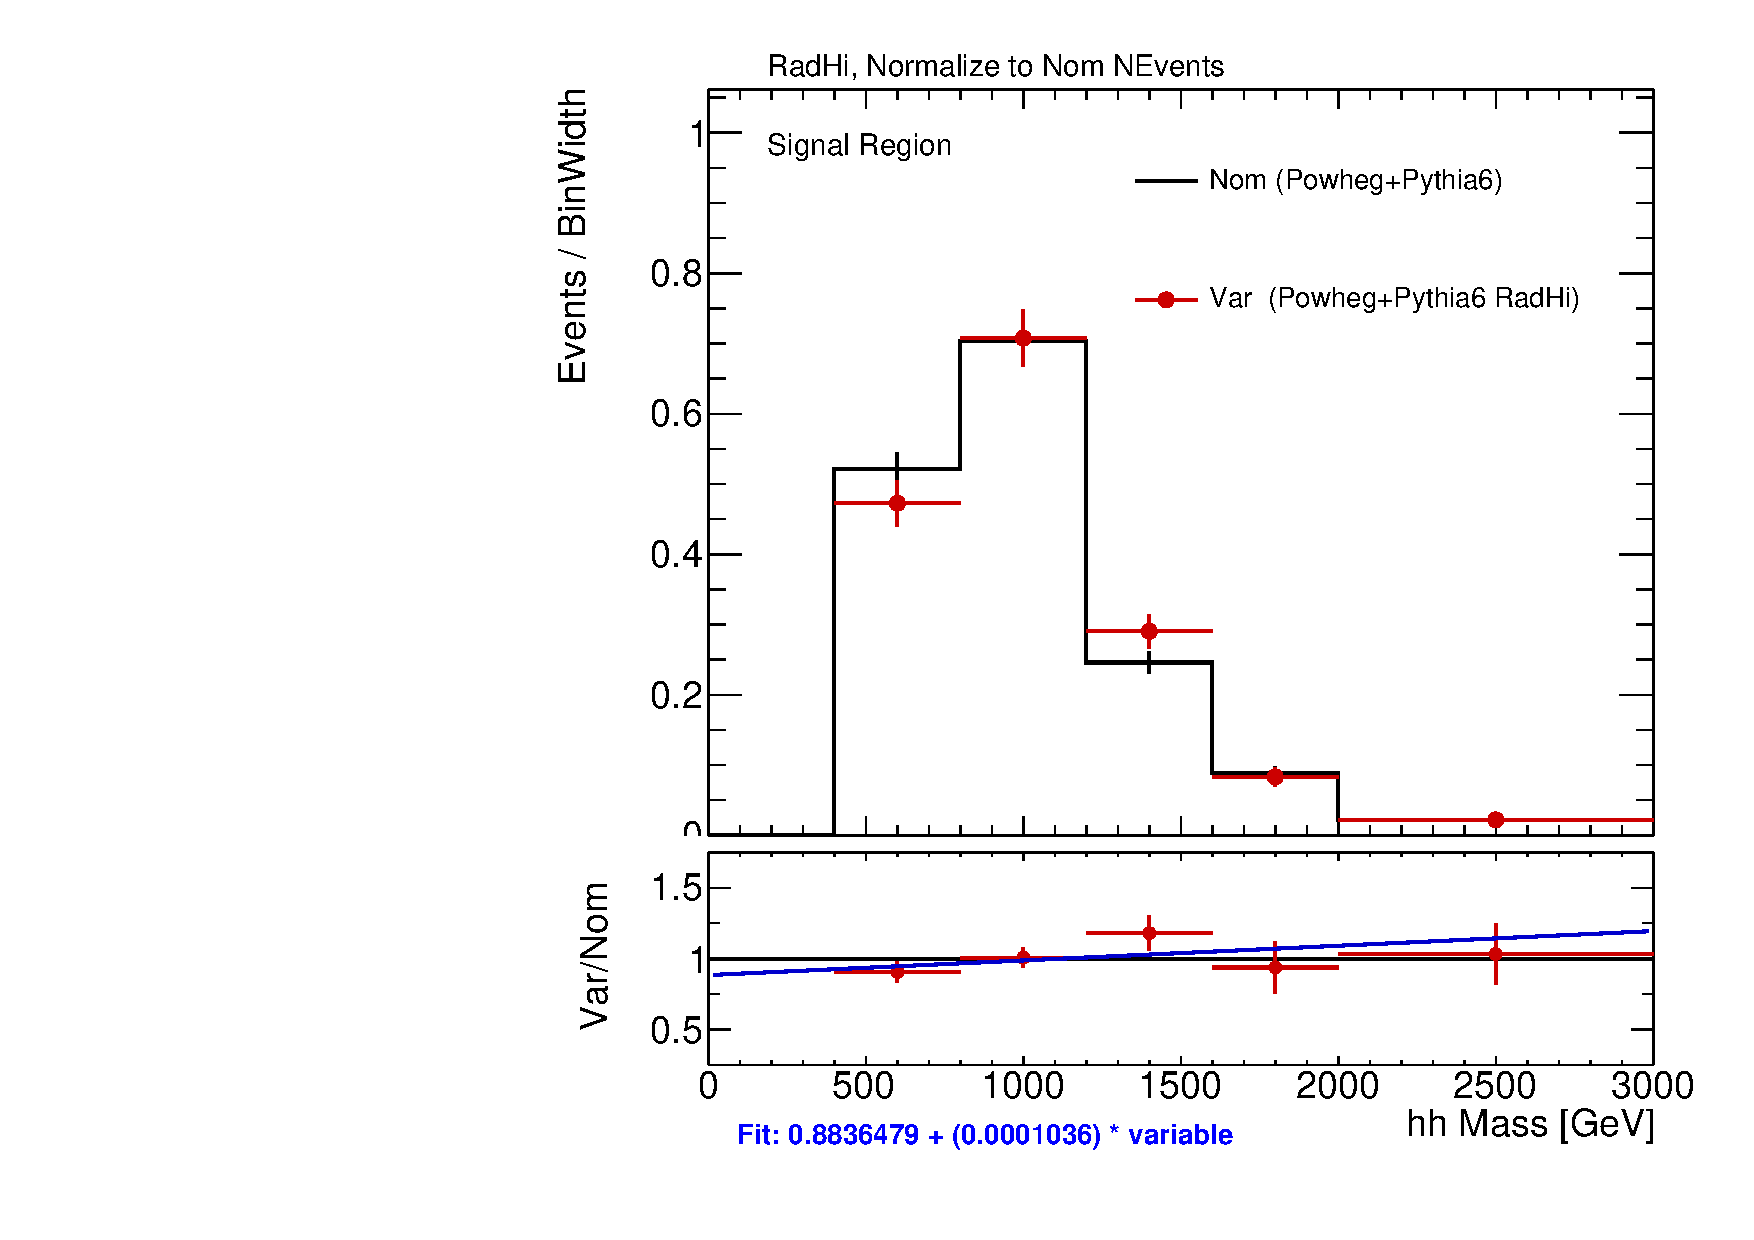
\includegraphics[scale=0.33]{./figures/boosted/systematics/ttbar_alt_hhMass_SR_RadHi_rebin} 
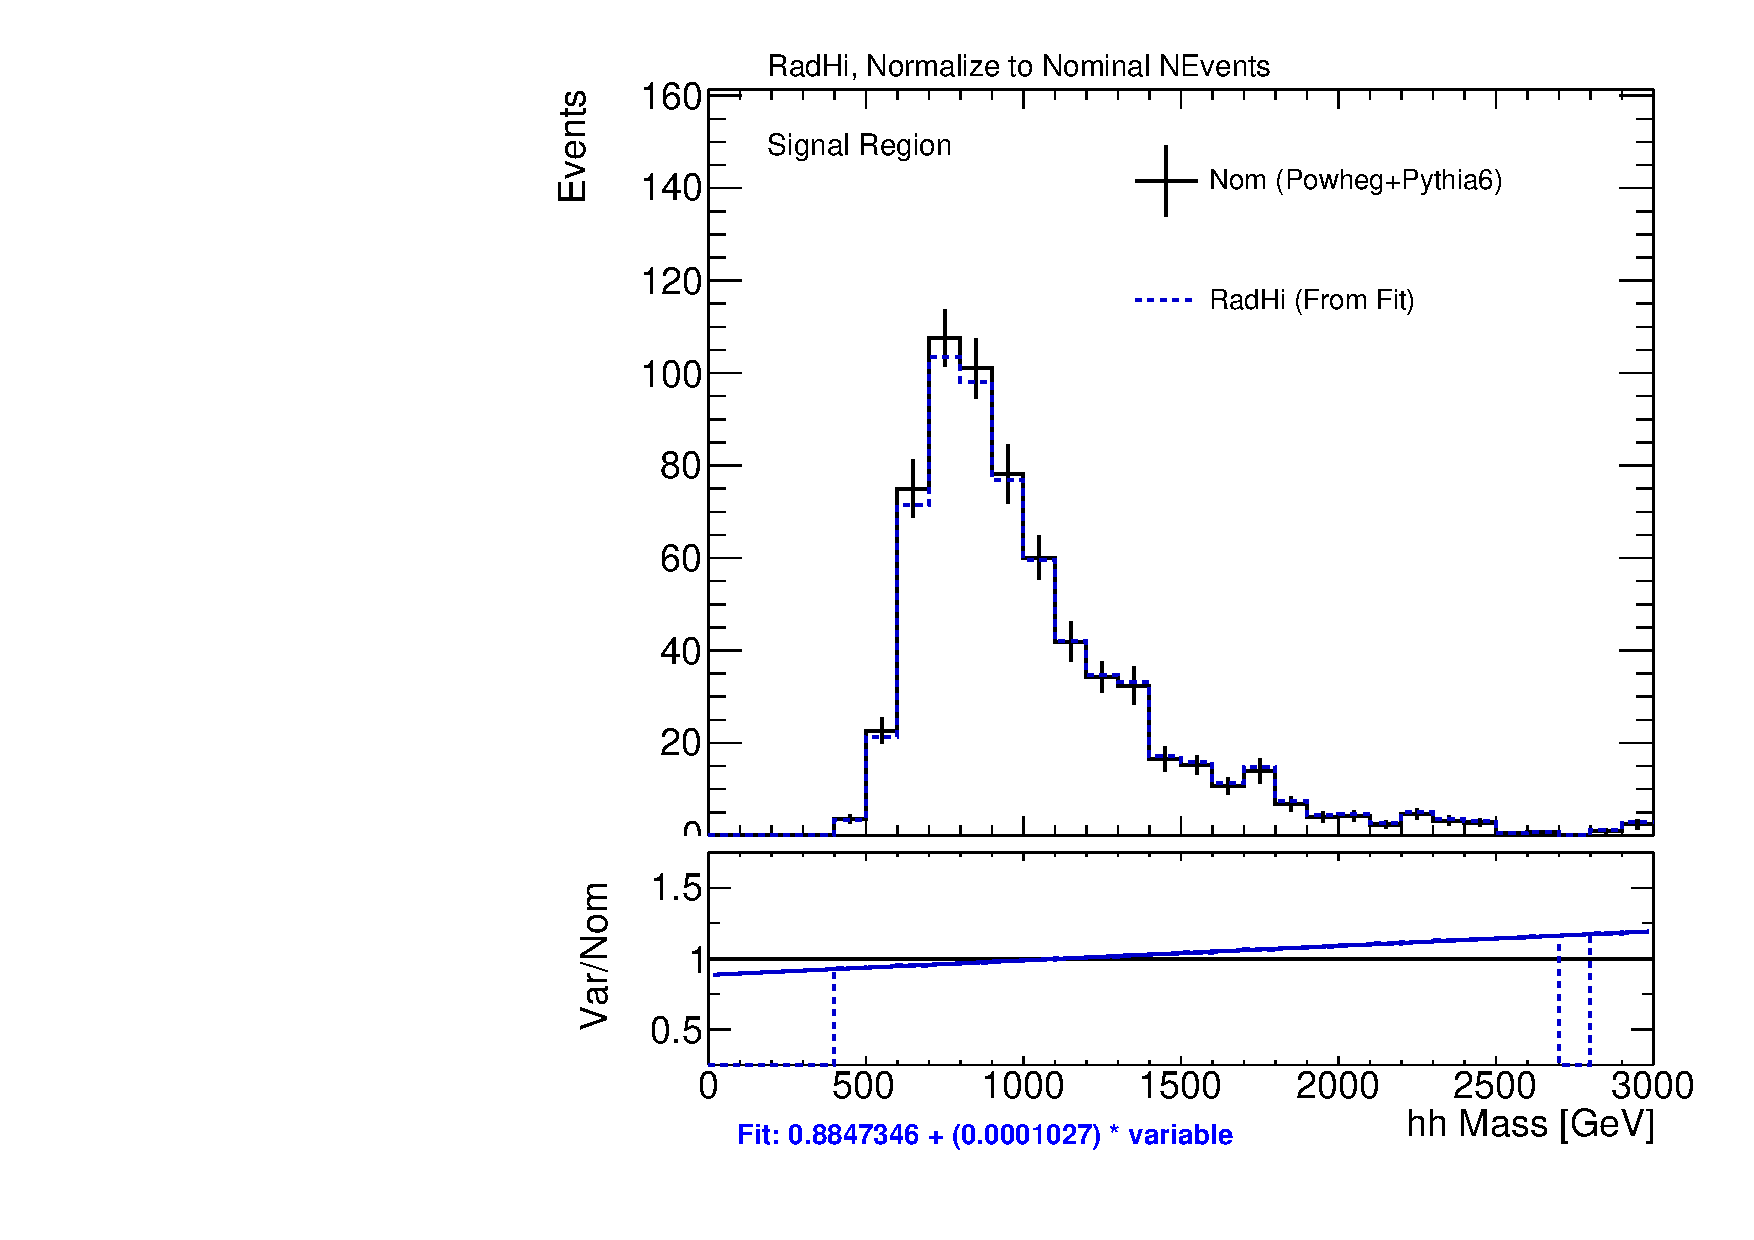
\includegraphics[scale=0.33]{./figures/boosted/systematics/ttbar_fromfit_hhMass_SR_RadHi}  \\
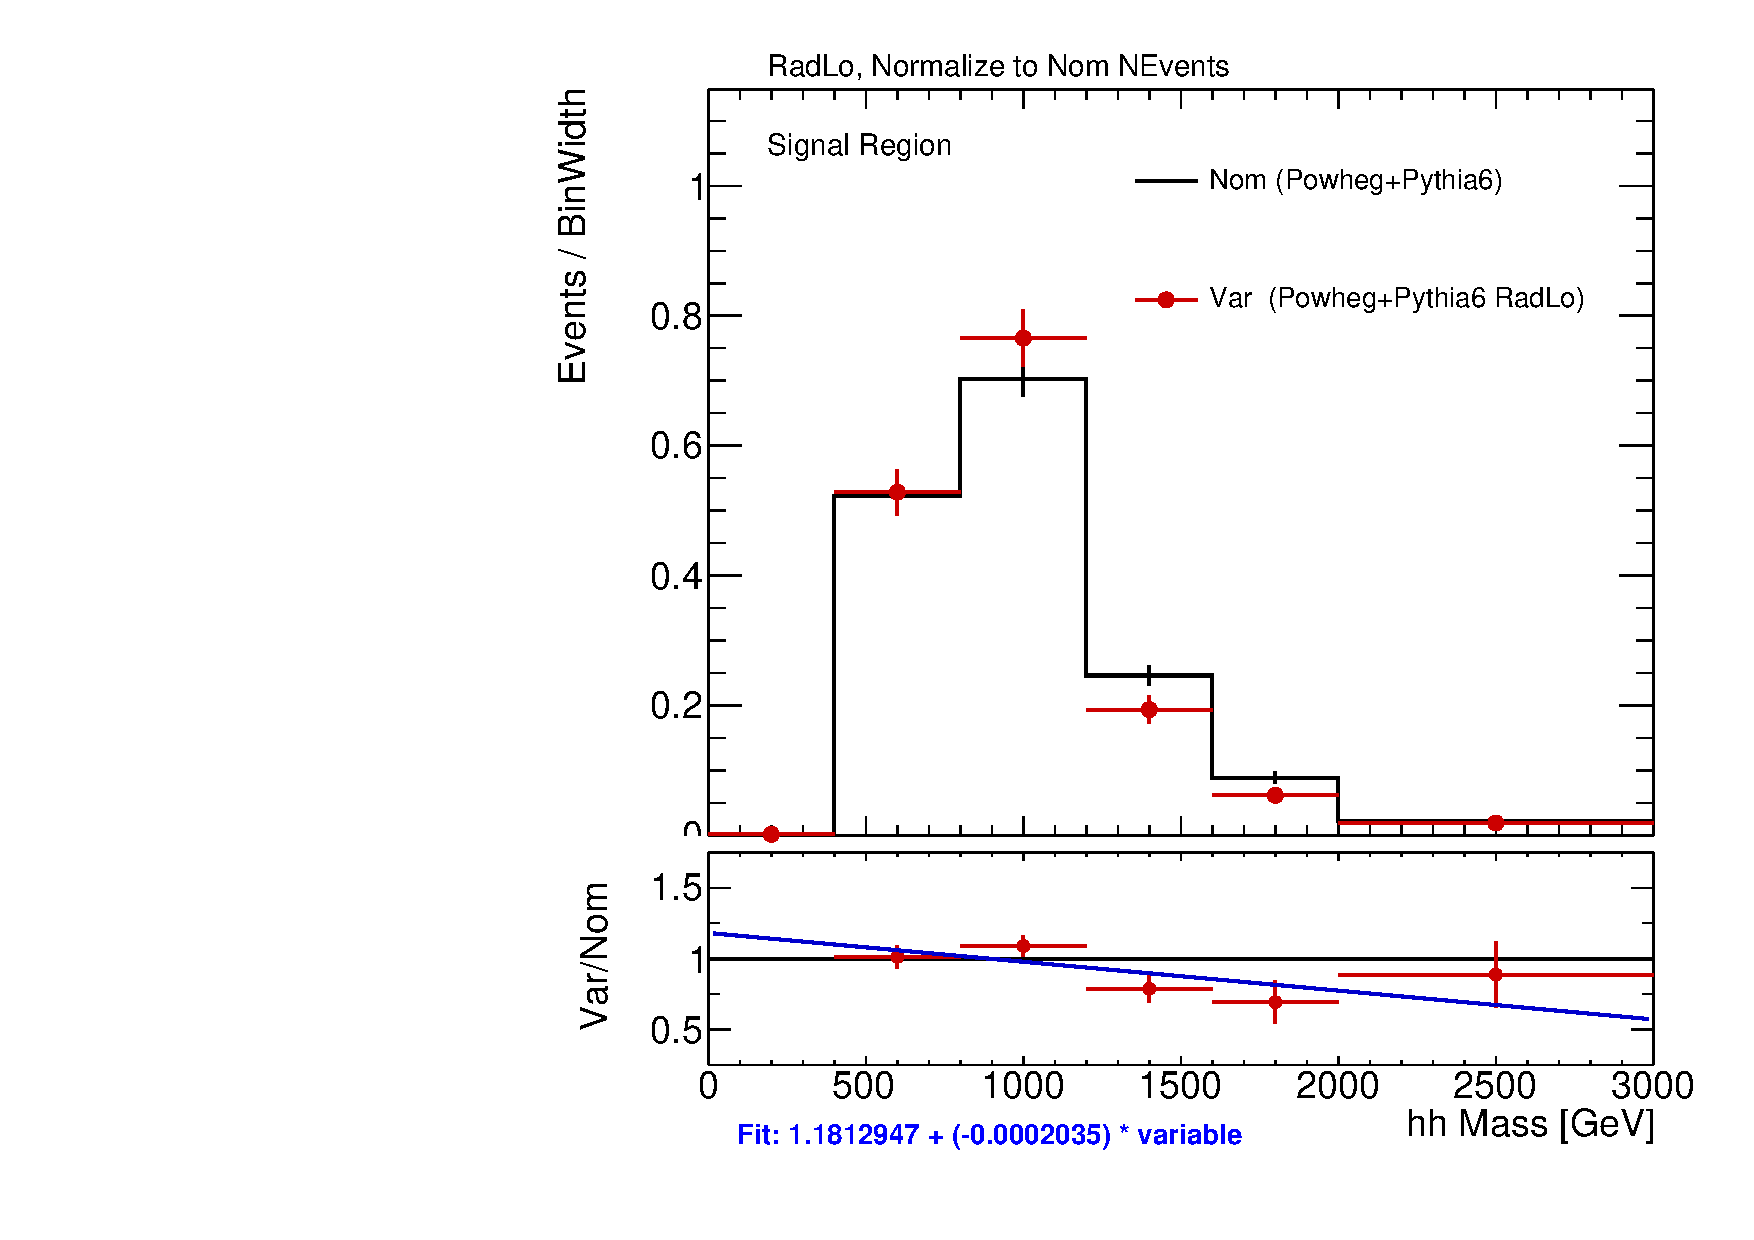
\includegraphics[scale=0.33]{./figures/boosted/systematics/ttbar_alt_hhMass_SR_RadLo_rebin}
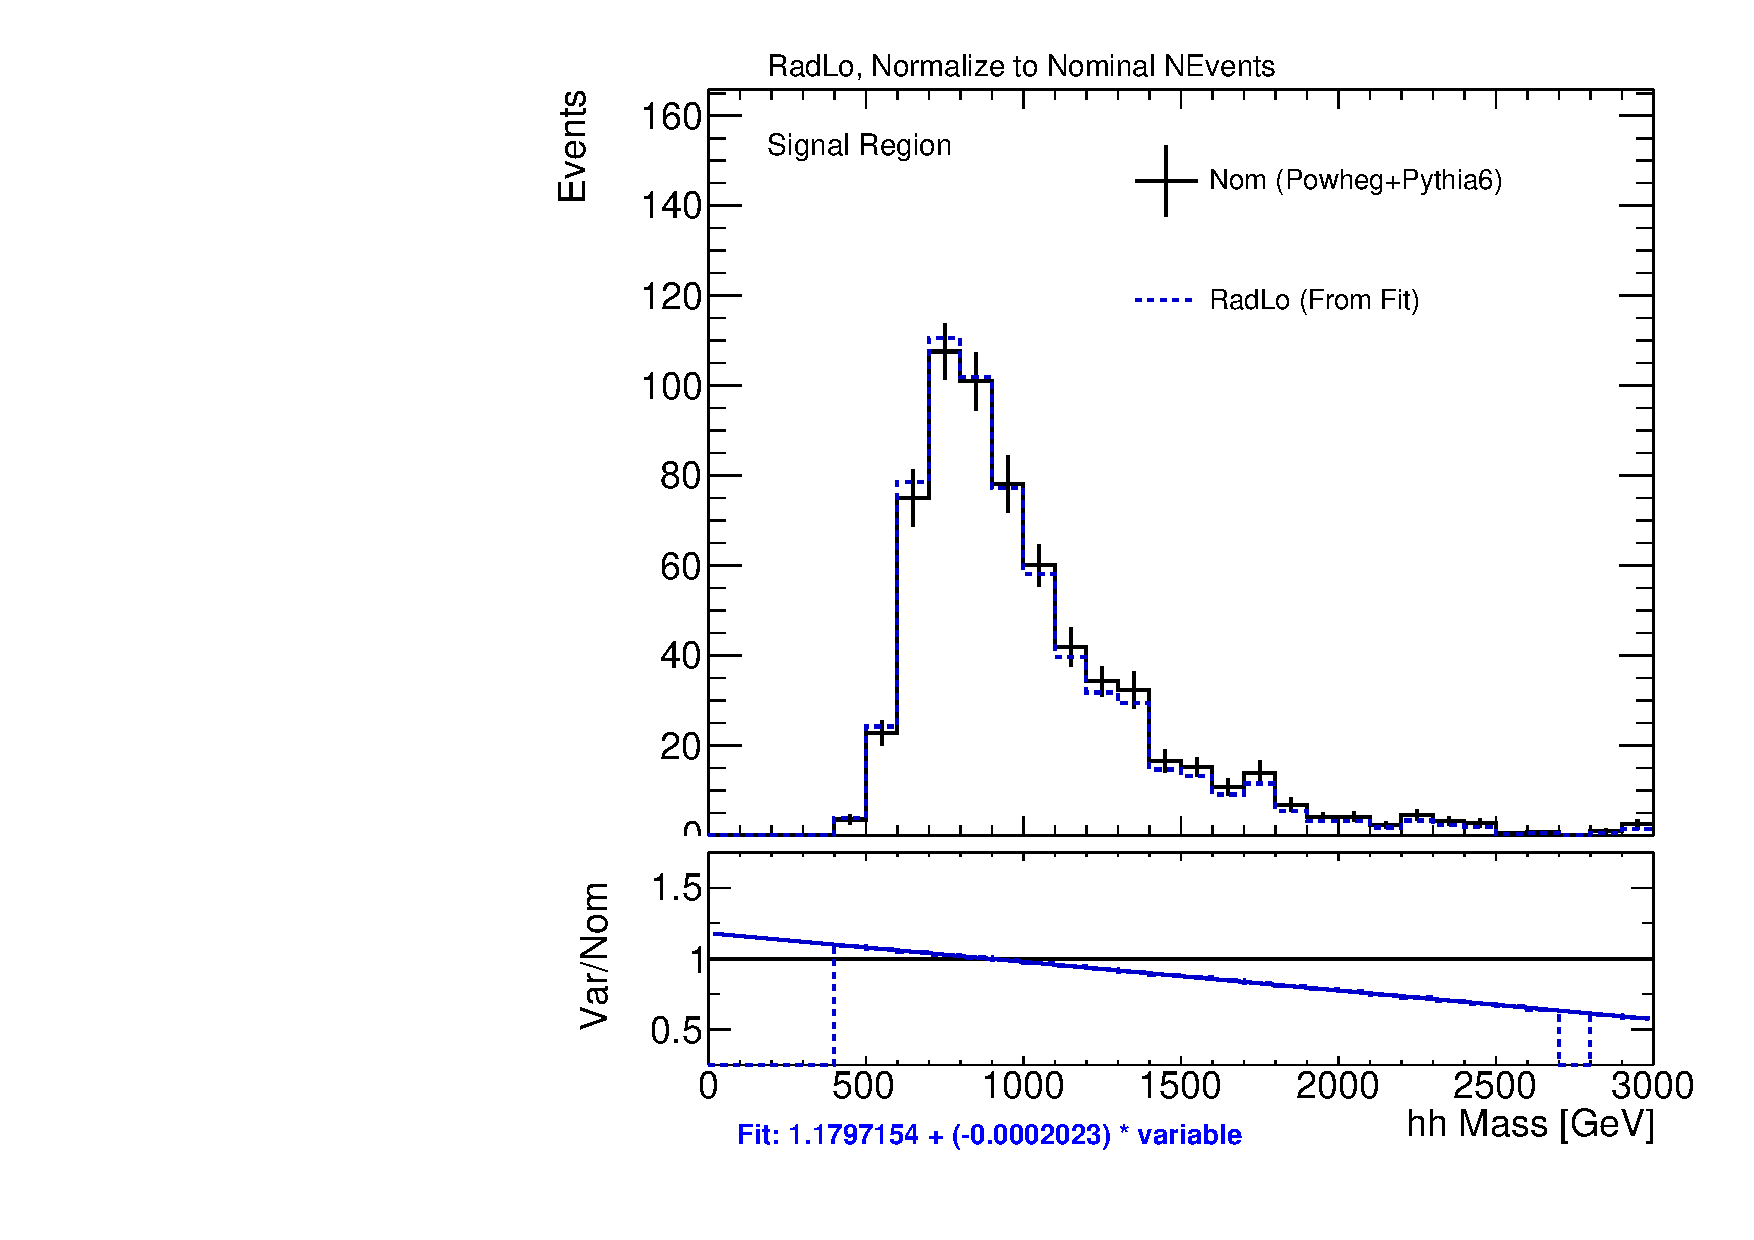
\includegraphics[scale=0.33]{./figures/boosted/systematics/ttbar_fromfit_hhMass_SR_RadLo}  \\
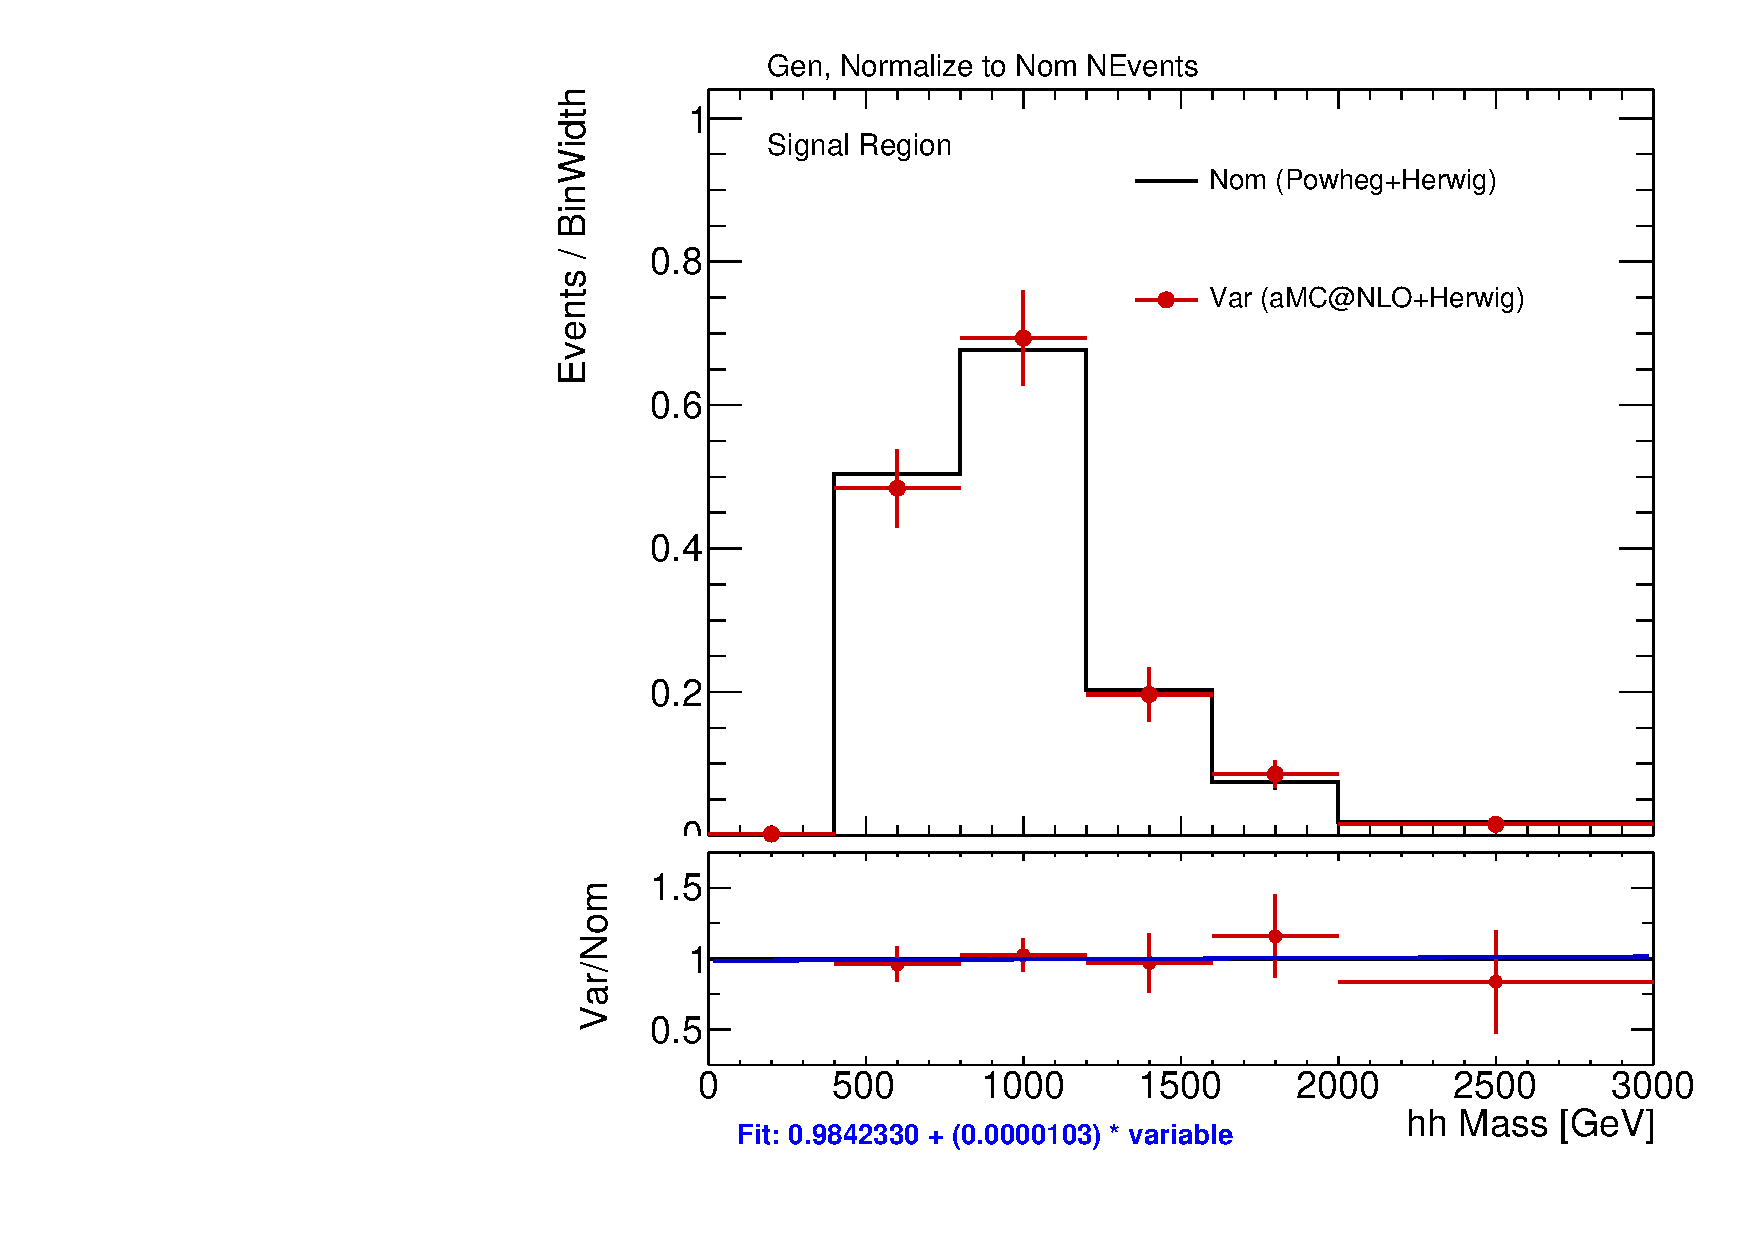
\includegraphics[scale=0.33]{./figures/boosted/systematics/ttbar_alt_hhMass_SR_Gen_rebin}  
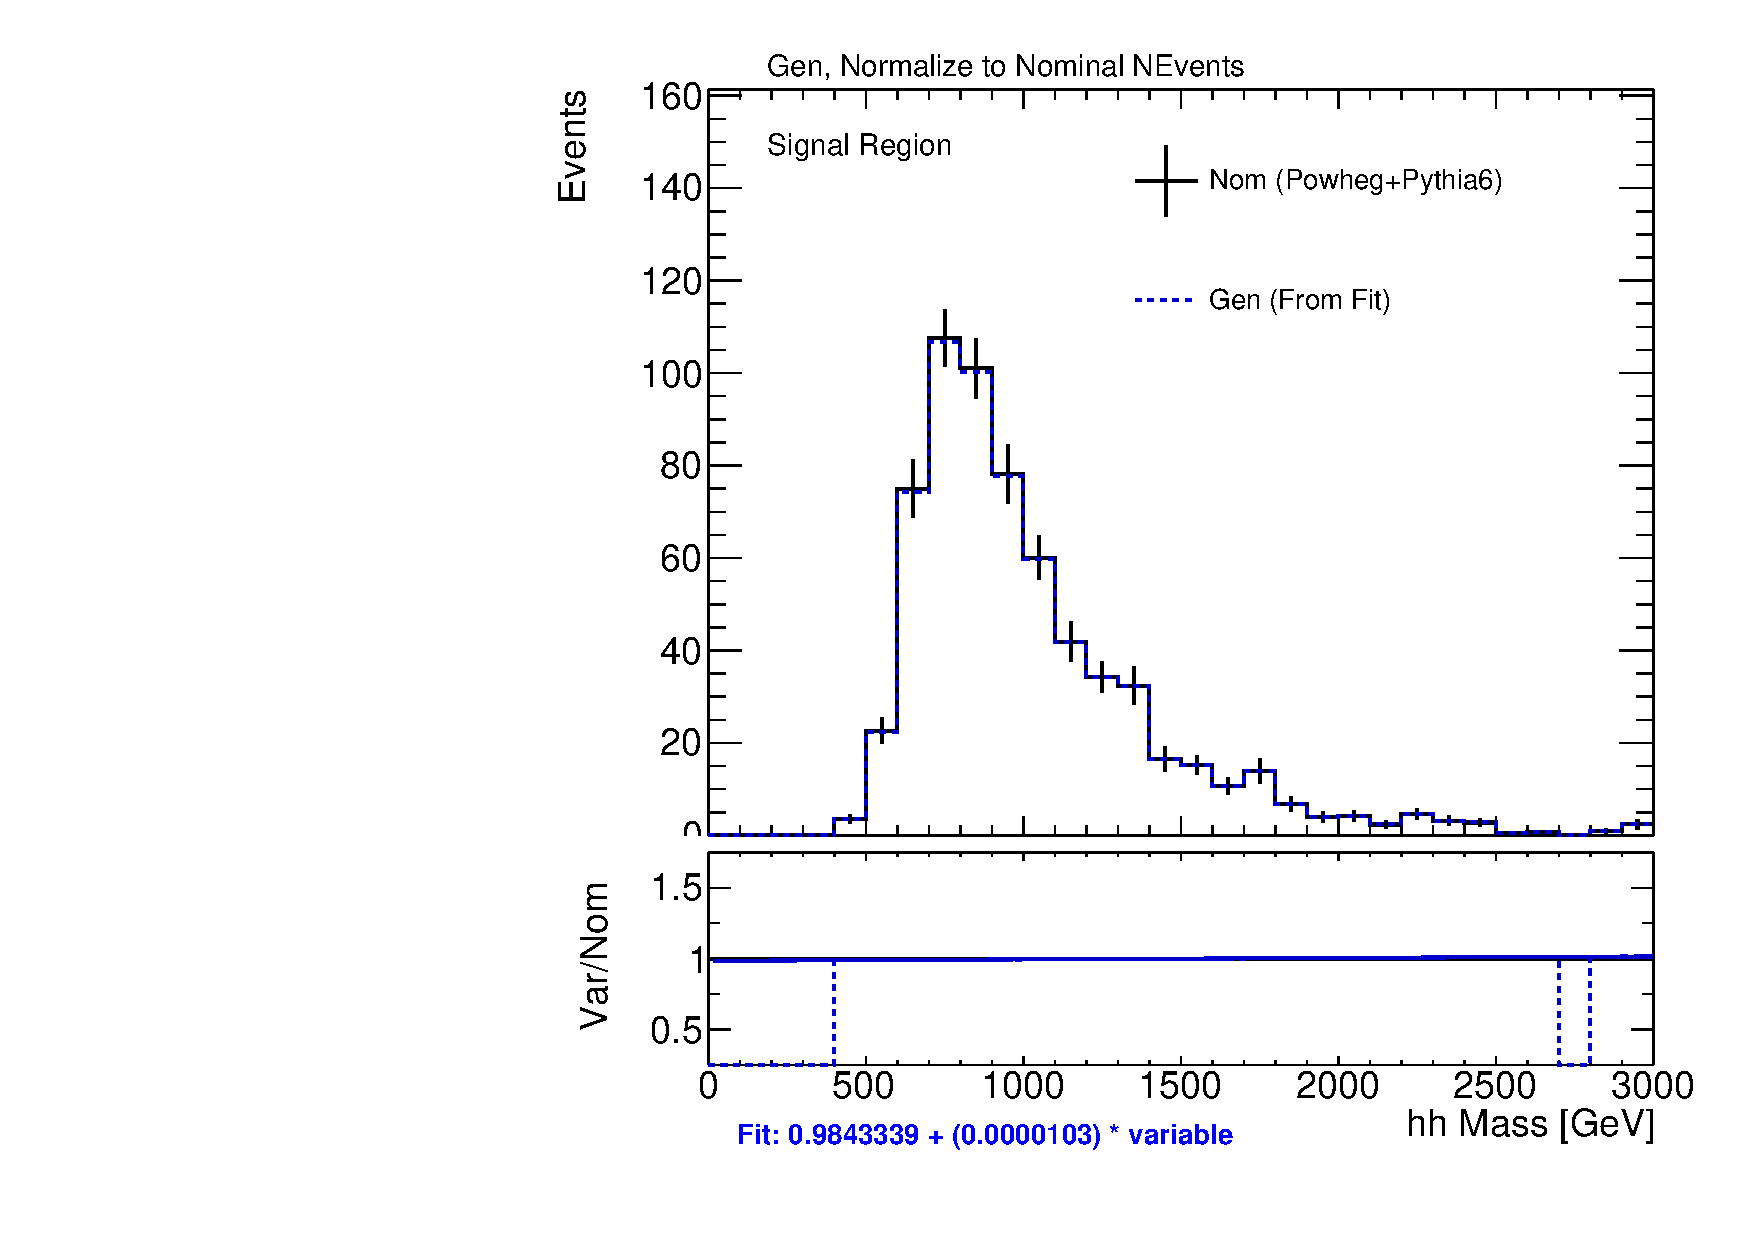
\includegraphics[scale=0.33]{./figures/boosted/systematics/ttbar_fromfit_hhMass_SR_Gen}     \\
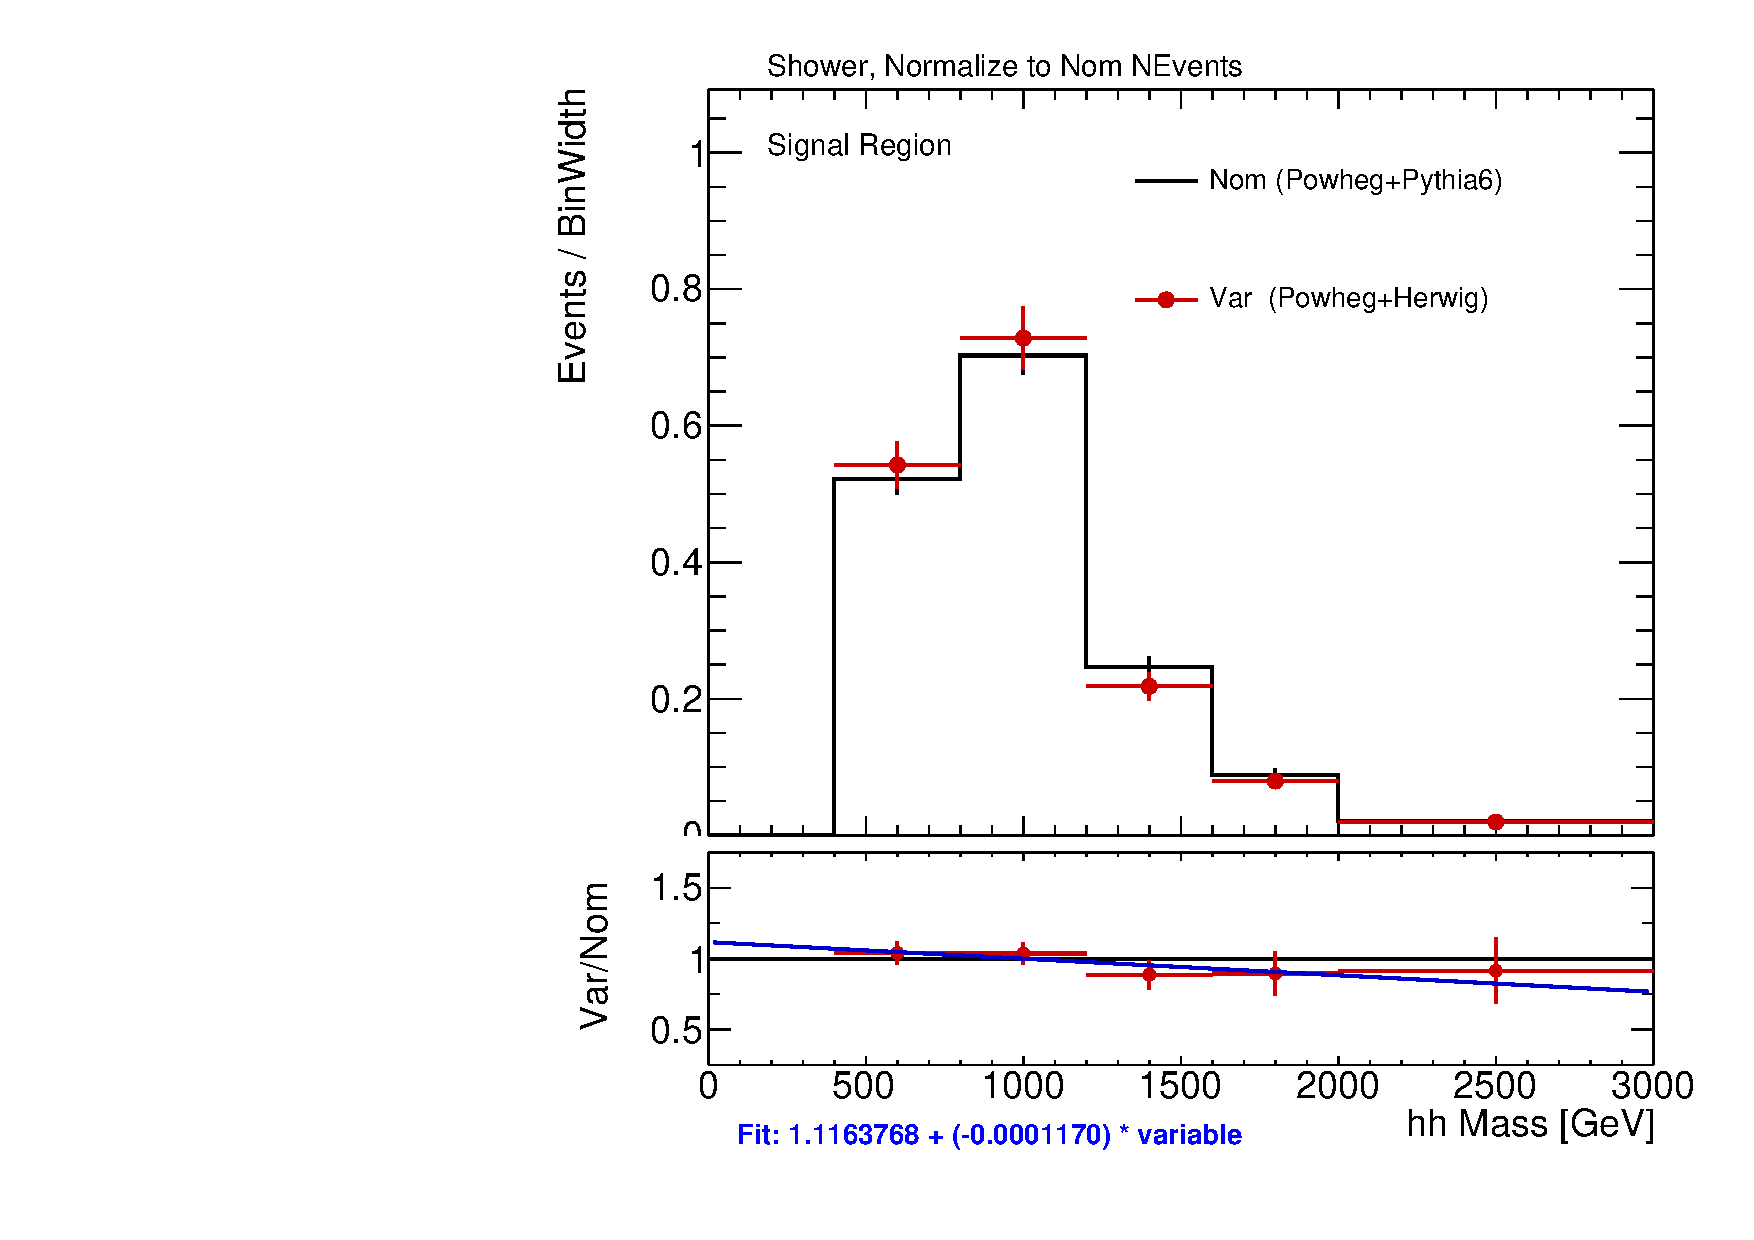
\includegraphics[scale=0.33]{./figures/boosted/systematics/ttbar_alt_hhMass_SR_Shower_rebin}
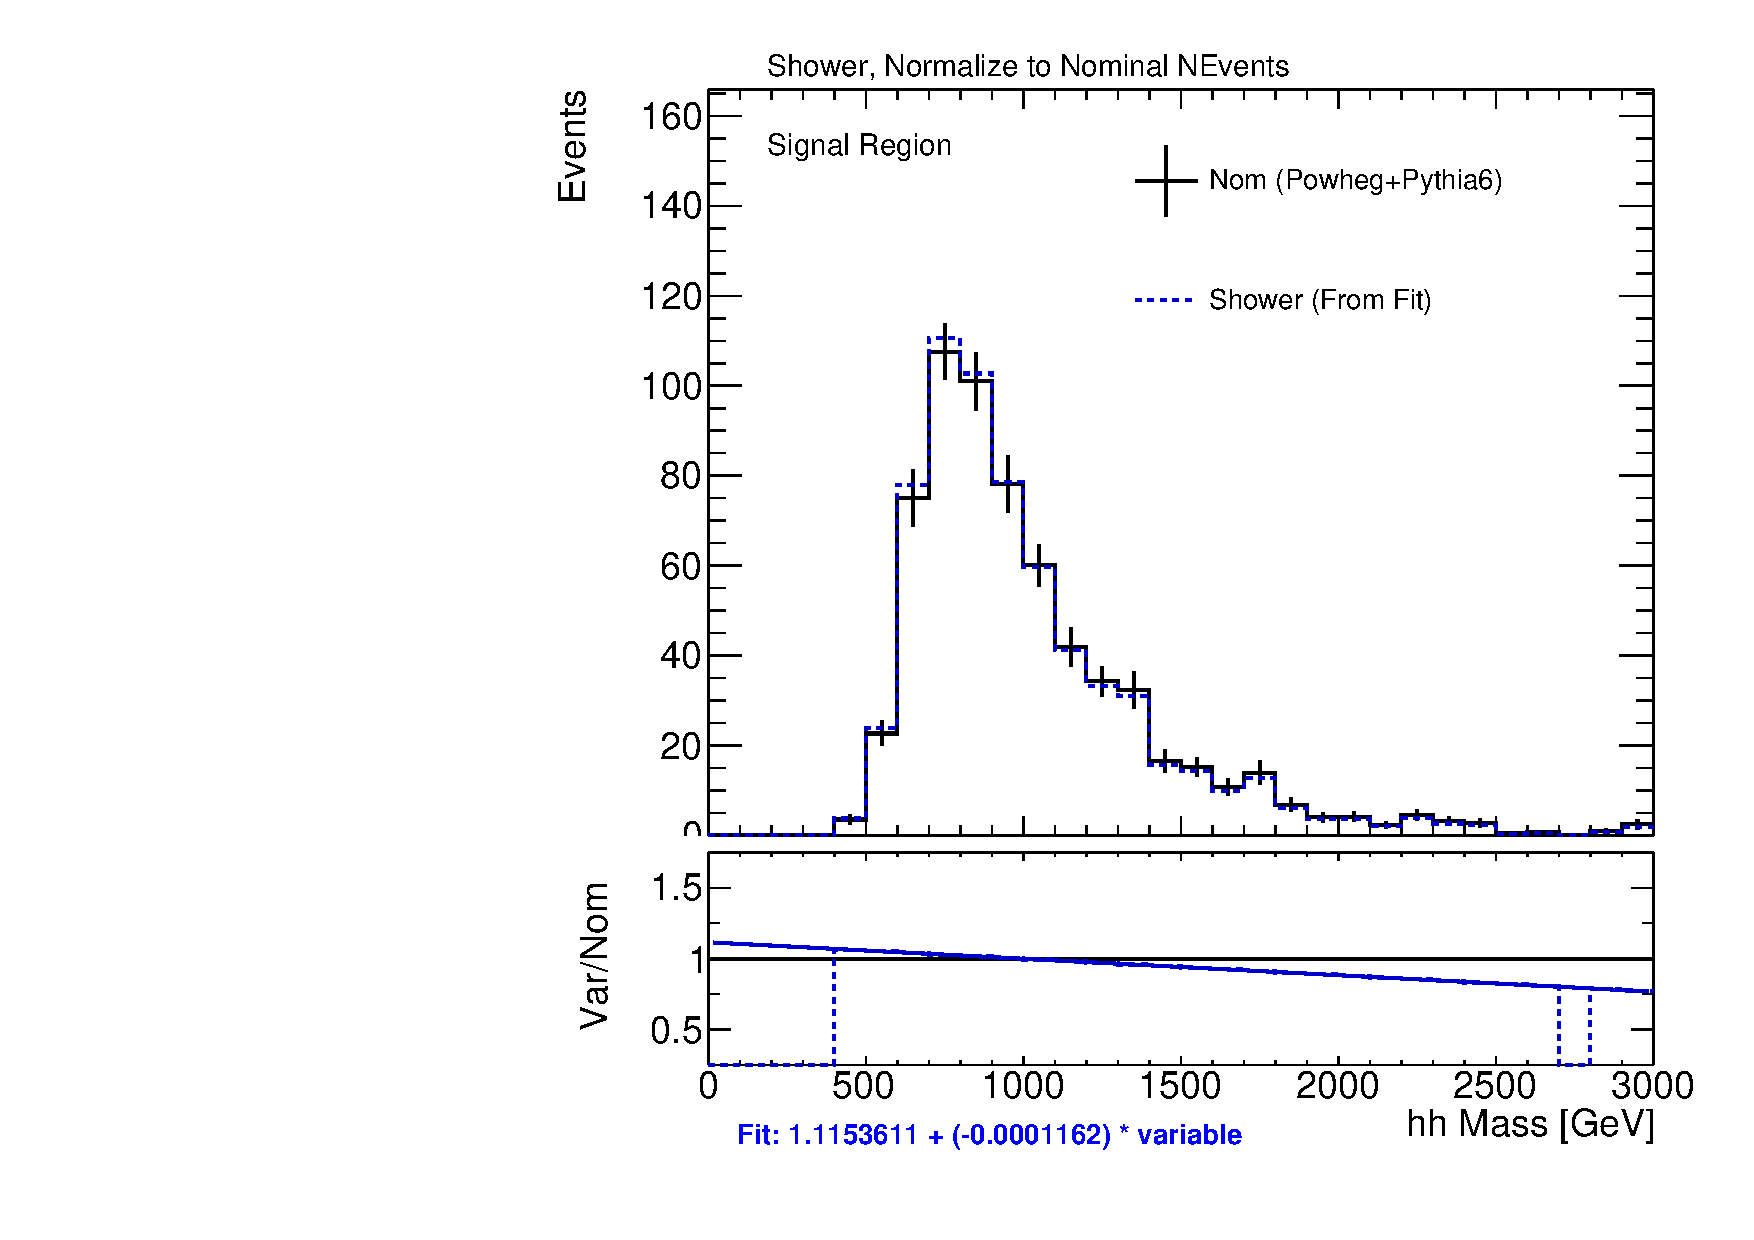
\includegraphics[scale=0.33]{./figures/boosted/systematics/ttbar_fromfit_hhMass_SR_Shower}   \\
\caption{$m_{hh}$ distribution shape comparison between nominal $t\bar{t}$ sample and alternative samples. Plot on the left is a direct
comparison between the nominal and alternative sample while on the right, the variation comes from the reweighted function applied to
the nominal $t\bar{t}$ sample. The linear fit in the ratio of the left plot is used as the reweighted function.}
\label{fig:boosted_unc_ttbar_shape_sr}
\end{center}
\end{figure}
 
For the single-top background, only the uncertainties on the modeling of the Wt production process are considered since it is the dominant single-top process in the
signal region. Table~\ref{tab:boosted_unc_singletopwt} shows the estimated uncertainty on the normalization of the single-top background. The biggest uncertainties comes from
the PS generator choice and comparisons to the DS sample. The total uncertainty is abnormally large, which is larger than 100\%.
 
\begin{table}[htbp!]
\begin{center}
\begin{tabular}{c|c}
Variation   &  Uncertainty (\%) \\
\hline
RadHi       &               15.1 \\
RadLo       &               19.0 \\
Herwig++    &               33.5 \\
DR          &               72.5 \\
aMC@NLO     &               25.4 \\
\hline
Total      &                85.9 \\
\end{tabular}
\end{center}
\caption{The normalization uncertainty for the $t\bar{t}$ background in the signal region
from different sources. The total uncertainty is calculated as the sum of quadrature from all
the sources.}
\label{tab:boosted_unc_singletopwt}
\end{table}
 
\FloatBarrier
 
%---------------------------------------------------------------------------------------------------------------
 
\paragraph{V+Jets processes}
\label{sec:boosted_syst_modeling_vjets}
 
The nominal V+Jets prediction, uses the ME+PS generator \SHERPA 2.2.1 interfaced with the NNPDF 3.0 NNLO PDF set.
This default configuration provides a prediction for vector boson production plus associated jets at NLO accuracy
at the ME level for up to 2 extra partons, and LO accuracy for 3 and 4 extra partons in QCD.
The merging of additional parton multiplicities arising from the internal \SHERPA PS, is regulated by the
MEPS@NLO merging technique.
 
The alternative samples used to assess the modeling uncertainties are:
 
\begin{itemize}
\item \textbf{MadGraph5+\PYTHIA8.186 :} The LO ME generator MadGraph5 using the NNPDF3.0(2.3) NLO(LO) PDF set interfaced
with \PYTHIA8 version 8.186 using the A14 tune, offers a LO+NLL accurate prediction for vector boson production in association
with jets for up to 4 extra partons from the ME and 4+ parton from \PYTHIA8 at NLL accuracy. The comparison between the nominal  
\SHERPA 2.2.1 sample with this sample convolves the ME and PS model variation. Due to the unavailability of this sample at
reconstruction level, the comparison is made at (particle) truth level.
 
\item \textbf{\SHERPA 2.2.1 scale variations:} Configured in the same manner as the nominal V+Jets sample,
the renormalisation $\mu_{R}$ and resummation $\mu_{F}$ scales are varied up/down by a factor of 2.
 
\item \textbf{\SHERPA 2.2.1 PDF variations:} Configured in the same manner as the nominal V+Jets sample. The
100 NNPDF3.0NNLO replicas variations are available. The central values of 2 alternative PDF sets, MMHT2014NNLO 68\%CL and CT14NNLO
are also available.
 
\item \textbf{\SHERPA 2.2.1 $\alpha_{s}(PDF)$ variations:} Configured in the same manner as the nominal V+Jets sample,
the $\alpha_{s}$ value used by the nominal NNPDF 3.0 NNLO PDF is varied up and down according to a variation of
the $\mu_{R}$ scale by a factor of 2.
\end{itemize}
 
Table~\ref{tab:boosted_unc_wjets} shows the estimated uncertainty on the normalization of the W+jets background in the signal region
from the comparison of the nominal W+jets sample to the alternative samples.  The largest uncertainty comes from the renormalization
and resummation scale, which is about \textasciitilde42\% and dominates the total uncertainty on W+jets background. The normalization of W+jets
background is assinged with a single nuisance parameter with the total uncertainty set as the prior uncertainty.
 
Shape comparisons of the $m_{hh}$ distribution between the nominal W+jets sample to the alternative samples were made and only one
variation was found to have noticeable difference: the scale variation of $\mu_{R}$=0.5, $\mu_{F}$=0.5 as in Figure~\ref{fig:boosted_unc_wjets_sr_scale_fit}.
Appendix~\ref{app:boosted_syst_wjets} documents studies on the normalization and shape systematics for W+jets background.
 
\begin{table}[htbp!]
\begin{center}
\begin{tabular}{c|c}
Variation  &  Uncertainty (\%) \\
\hline
Scale                 &   41.9  \\
$\alpha_{S}$(PDF)     &   8.4   \\
PDF alternative set   &   1.6   \\
NNPDF replicas        &   5.6   \\
Madgraph+Pythia8      &   11.0   \\
\hline
Total                 &   44.5  \\
\end{tabular}
\end{center}
\caption{The normalization uncertainty for the W+jets background in the signal region
from different sources. The total uncertainty is calculated as the sum of quadrature from all
the sources.}
\label{tab:boosted_unc_wjets}
\end{table}
 
\begin{figure}[!htbp]
\begin{center}
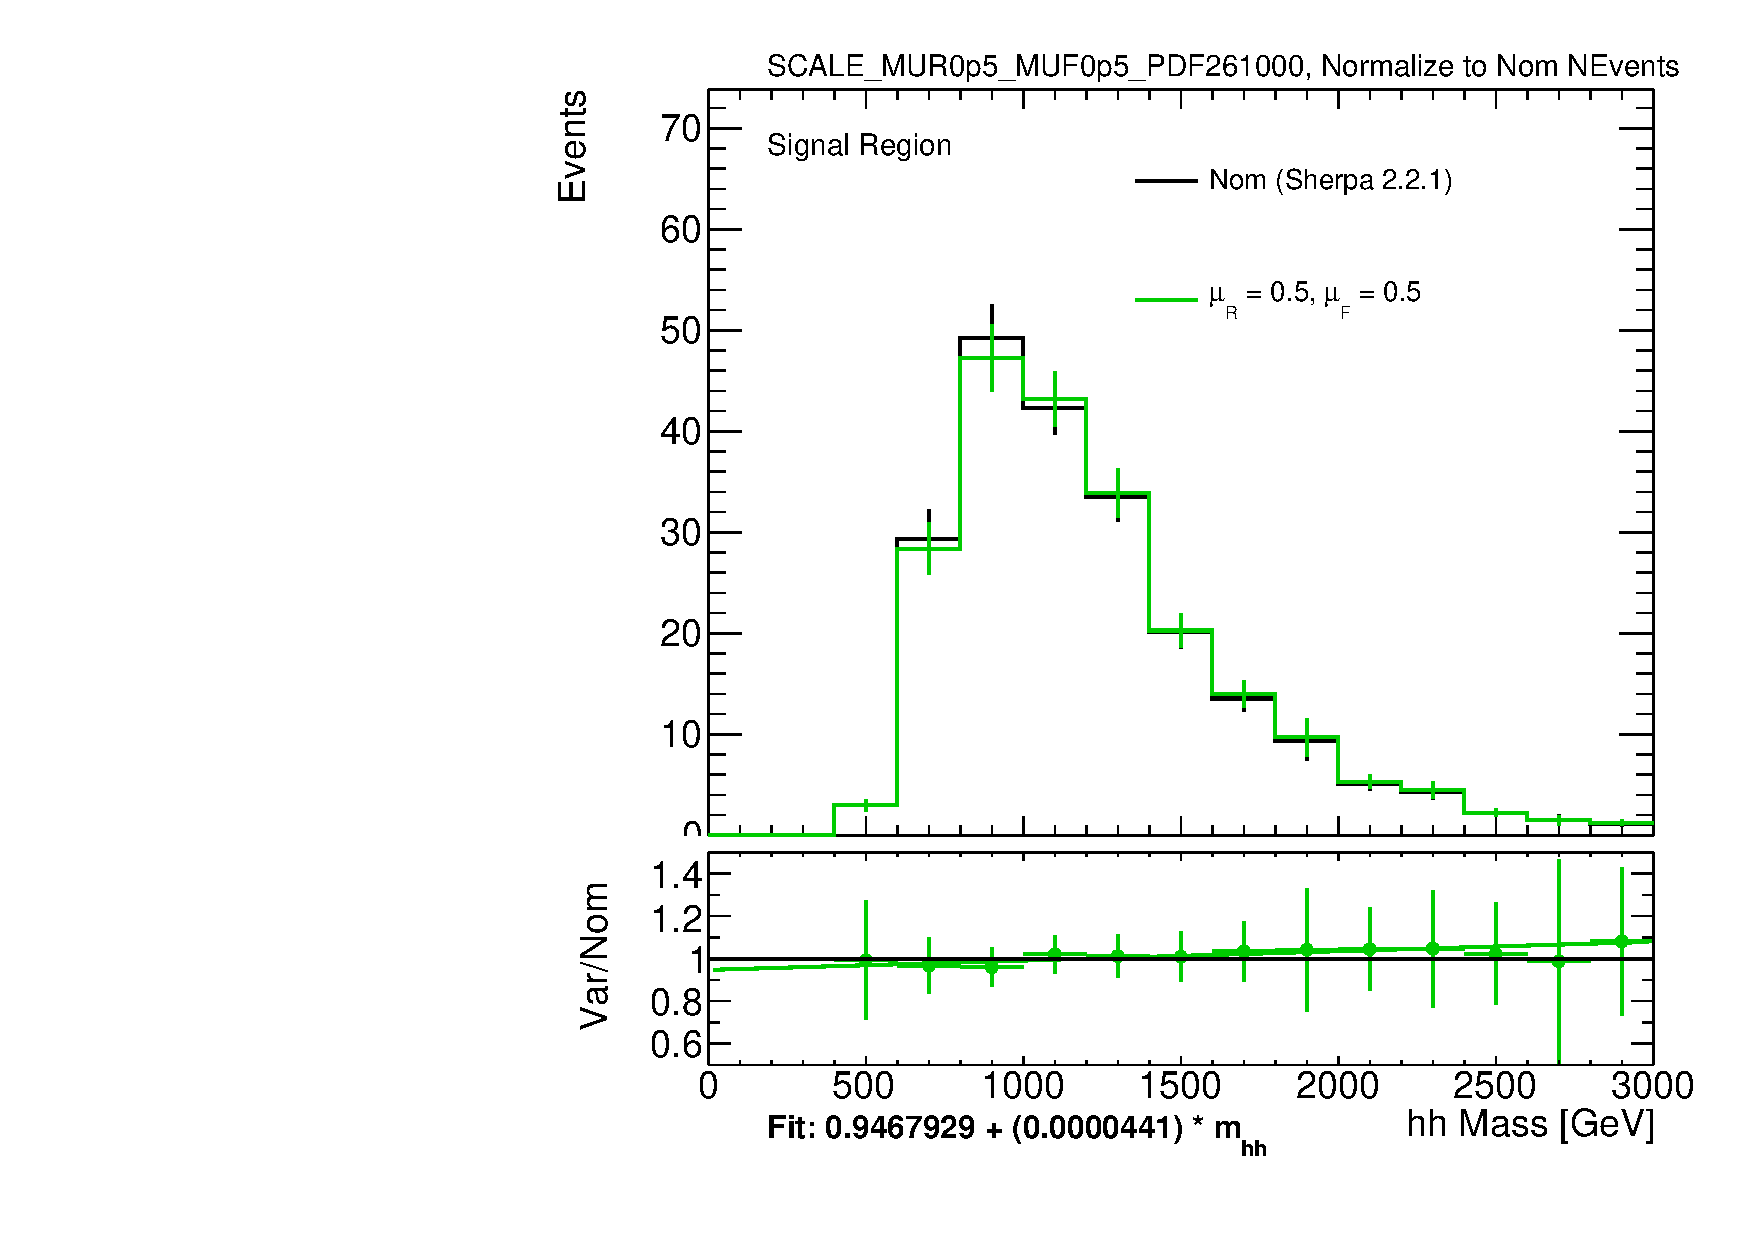
\includegraphics[scale=0.33]{./figures/boosted/systematics/wjets_alt_hhMass_SR_syst_SCALE_MUR0p5_MUF0p5_PDF261000}
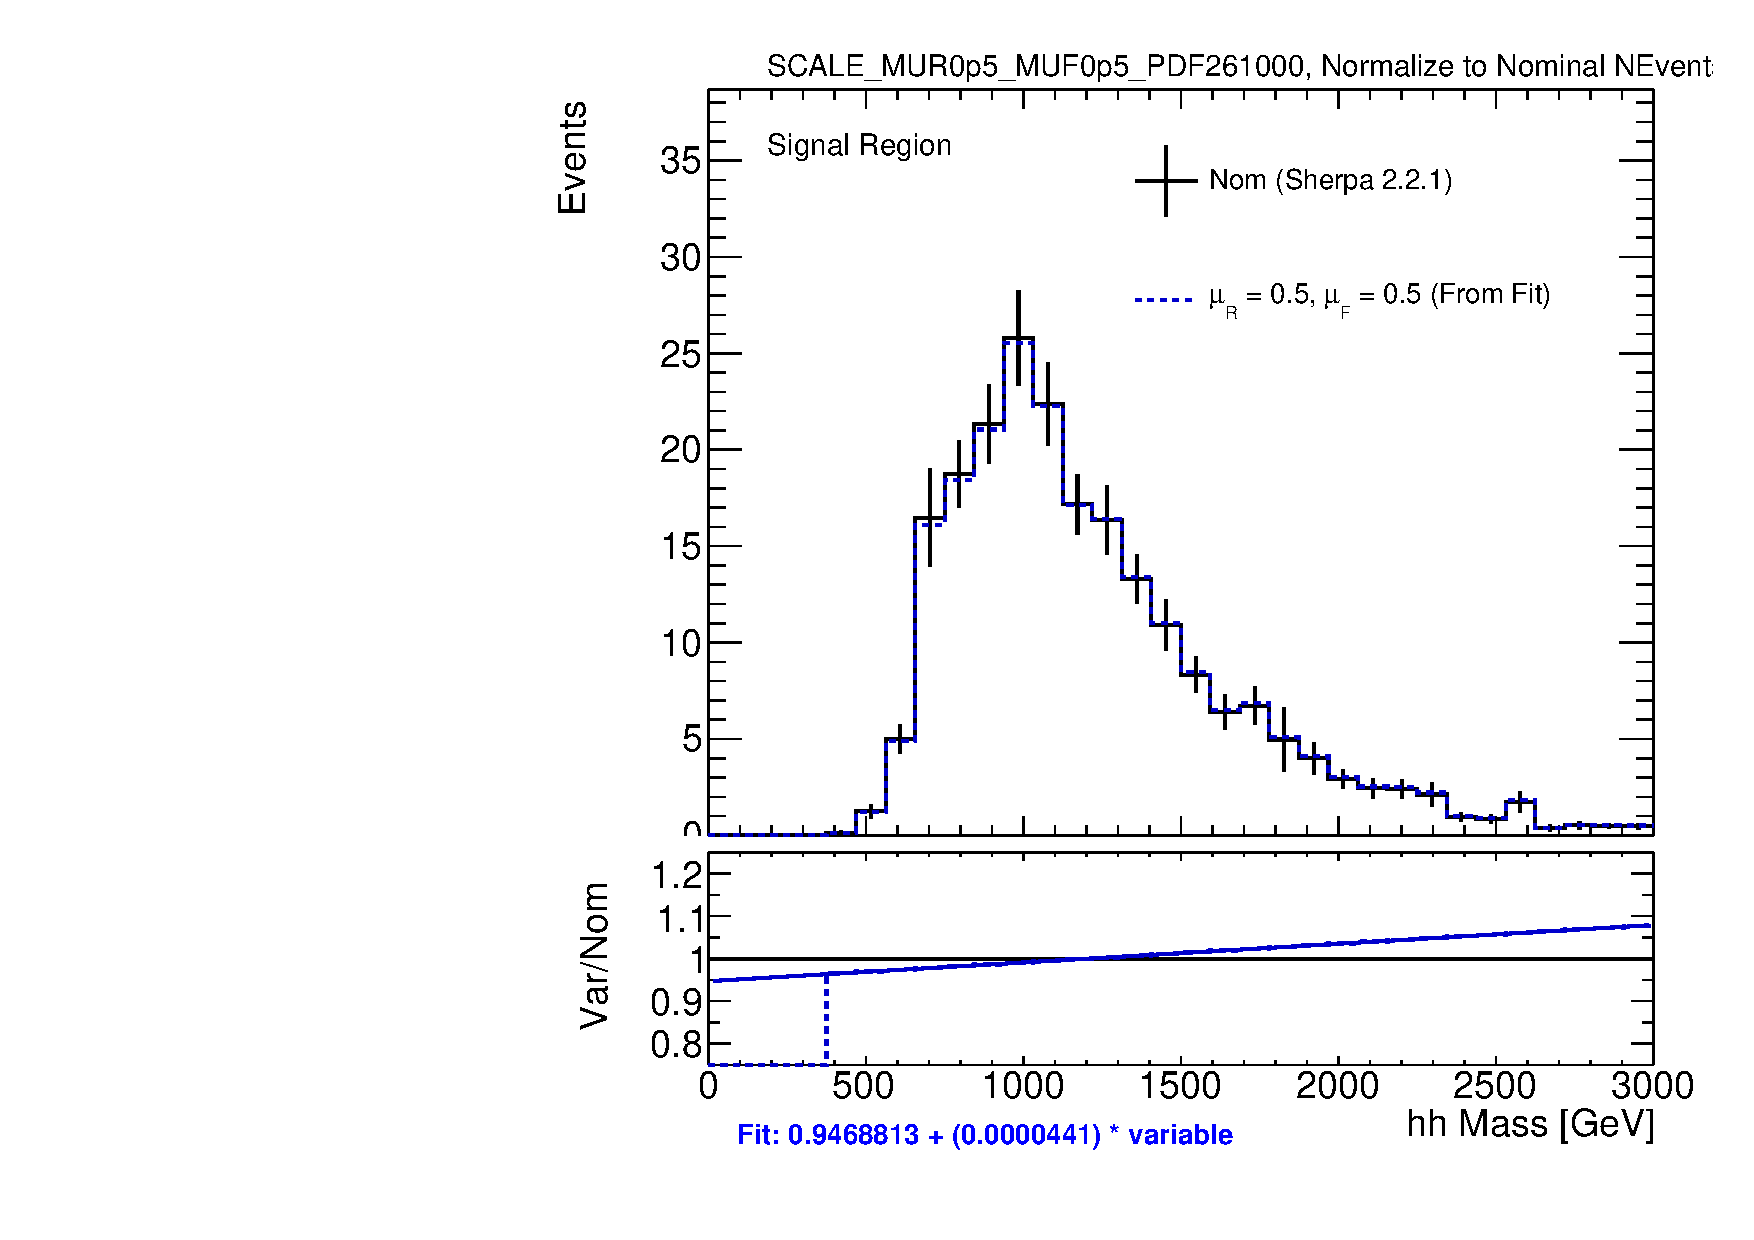
\includegraphics[scale=0.33]{./figures/boosted/systematics/wjets_fromfit_hhMass_SR_SCALE_MUR0p5_MUF0p5_PDF261000} \\
\caption{$m_{hh}$ distribution shape comparison between nominal W+jets sample and scale variation ($\mu_{R}$=0.5, $\mu_{F}$=0.5) sample. Plot on the left is a direct
comparison between the nominal and variation sample while on the right, the variation comes from the reweighted function applied to the nominal W+jets sample. The linear fit
in the ratio of the left plot is used as the reweighted function.}
\label{fig:boosted_unc_wjets_sr_scale_fit}
\end{center}
\end{figure}
 
Table~\ref{tab:boosted_unc_zjets} shows the estimated uncertainty on the normalization of the Z+jets background in the signal region
from the comparison of the nominal Z+jets sample to the alternative samples. The largest uncertainty comes from the renormalization
and resummation scale, which is about \textasciitilde48\% and dominates the total uncertainty on Z+jets background. The normalization of Z+jets
background is assinged with a single nuisance parameter with the total uncertainty set as the prior uncertainty. The uncertainty on the
$m_{hh}$ shape is found to be negligible and therefore ignored. Appendix~\ref{app:boosted_syst_zjets} documents studies on the normalization
and shape systematics for Z+jets background.
 
\begin{table}[htbp!]
\begin{center}
\begin{tabular}{c|c}
Variation  &  Uncertainty (\%) \\
\hline
Scale               &   48.3  \\
$\alpha_{S}$(PDF)   &   1.6   \\
PDF alternative set &   2.7   \\
NNPDF replicas      &   1.4   \\
\hline
Total               &   48.4  \\
\end{tabular}
\end{center}
\caption{The normalization uncertainty for the Z+jets background in the signal region
from different sources. The total uncertainty is calculated as the sum of quadrature from all
the sources.}
\label{tab:boosted_unc_zjets}
\end{table}
 
\FloatBarrier
%---------------------------------------------------------------------------------------------------------------
\paragraph{Diboson processes}
\label{sec:boosted_syst_modeling_diboson}
The systematic uncertainty on the normalization of the Diboson background is assigned to be 40\%. This uncertainty
is taken from the resolved analysis. As the background is small, the uncertainty is considered to be conservative.
 
%---------------------------------------------------------------------------------------------------------------
\paragraph{production}
\label{sec:boosted_syst_modeling_signal}
Systematic uncertainties on the acceptance of signal processes are computed by generating alternative variation signal samples
and then compare their acceptance with respect to the nominal signal samples. The difference sources of uncertainty considered are:
 
\begin{itemize}
\item \textbf{Scale variations:} Configured in the same manner as the nominal signal samples but
the renormalisation and resummation scales are varied up/down by a factor of 2.
 
% \item \textbf{PDF:}
 
\item \textbf{Parton shower choice:} Configured in the same manner as the nominal signal samples but
with Pythia 8 chosen as the shower generator instead of Herwig++.
\end{itemize}
 
Table~\ref{tab:boosted_unc_signal} lists the systematic uncertainties for 4 different scalar signal sample
mass points.
 
\begin{table}[htbp!]
\begin{center}
\begin{tabular}{c|c|c|c|c|c}
Variation    &  Xhh1000  &  Xhh1500 & Xhh2000 & Xhh2500 & Xhh3000   \\
\hline
Scale        &    0.2    &    0.2   &  0.4    &  0.4   &  0.4  \\
PDF          &    0.4    &    0.2   &  0.4    &  0.2   &  0.1  \\
Shower       &    0.4    &    0.8   &  1.6    &  3.4   &  4.1  \\
\end{tabular}
\end{center}
\caption{Theoretical uncertainties (in percentage) on the acceptance of several signal mass points.}
\label{tab:boosted_unc_signal}
 
 
\end{table}
%---------------------------------------------------------------------------------------------------------------
\subsubsection{QCD multijet modeling}
\label{sec:boosted_syst_modeling_multijet}
 
Systematic uncertainties related to the modeling of the multijet background were discussed in Section~\ref{sec:boosted_bkgd_qcdmultijet_yield_unc}
for the predicted yield and in Section~\ref{sec:boosted_bkgd_qcdmultijet_yield_unc} for the predicted $m_{hh}$ distribution.